
\documentclass{article}
\usepackage[english]{babel}
\usepackage[utf8]{inputenc}
\usepackage[english]{babel}
\usepackage[a4paper, total={7.25in, 9.5in}]{geometry}
\usepackage{tikz-feynman}
\tikzfeynmanset{compat=1.0.0} 
\usepackage{subcaption}
\usepackage{float}
\floatplacement{figure}{H}
\usepackage{simpler-wick}
\usepackage{mathrsfs}  
\usepackage{dsfont}
\usepackage{relsize}
\usepackage{tikz-cd}
\DeclareMathAlphabet{\mathdutchcal}{U}{dutchcal}{m}{n}

\usepackage{cancel}



\newcommand{\field}{\hat{\Phi}}
\newcommand{\dfield}{\hat{\Phi}^\dagger}
 
\usepackage{amsthm, amssymb, amsmath, centernot}
\usepackage{slashed}
\newcommand{\notimplies}{%
  \mathrel{{\ooalign{\hidewidth$\not\phantom{=}$\hidewidth\cr$\implies$}}}}
 
\renewcommand\qedsymbol{$\square$}
\newcommand{\cont}{$\boxtimes$}
\newcommand{\divides}{\mid}
\newcommand{\ndivides}{\centernot \mid}

\newcommand{\Integers}{\mathbb{Z}}
\newcommand{\Natural}{\mathbb{N}}
\newcommand{\Complex}{\mathbb{C}}
\newcommand{\Zplus}{\mathbb{Z}^{+}}
\newcommand{\Primes}{\mathbb{P}}
\newcommand{\Q}{\mathbb{Q}}
\newcommand{\R}{\mathbb{R}}
\newcommand{\ball}[2]{B_{#1} \! \left(#2 \right)}
\newcommand{\Rplus}{\mathbb{R}^+}
\renewcommand{\Re}[1]{\mathrm{Re}\left[ #1 \right]}
\renewcommand{\Im}[1]{\mathrm{Im}\left[ #1 \right]}
\newcommand{\Op}{\mathcal{O}}

\newcommand{\invI}[2]{#1^{-1} \left( #2 \right)}
\newcommand{\End}[1]{\text{End}\left( A \right)}
\newcommand{\legsym}[2]{\left(\frac{#1}{#2} \right)}
\renewcommand{\mod}[3]{\: #1 \equiv #2 \: \mathrm{mod} \: #3 \:}
\newcommand{\nmod}[3]{\: #1 \centernot \equiv #2 \: mod \: #3 \:}
\newcommand{\ndiv}{\hspace{-4pt}\not \divides \hspace{2pt}}
\newcommand{\finfield}[1]{\mathbb{F}_{#1}}
\newcommand{\finunits}[1]{\mathbb{F}_{#1}^{\times}}
\newcommand{\ord}[1]{\mathrm{ord}\! \left(#1 \right)}
\newcommand{\quadfield}[1]{\Q \small(\sqrt{#1} \small)}
\newcommand{\vspan}[1]{\mathrm{span}\! \left\{#1 \right\}}
\newcommand{\galgroup}[1]{Gal \small(#1 \small)}
\newcommand{\bra}[1]{\left| #1 \right>}
\newcommand{\Oa}{O_\alpha}
\newcommand{\Od}{O_\alpha^{\dagger}}
\newcommand{\Oap}{O_{\alpha '}}
\newcommand{\Odp}{O_{\alpha '}^{\dagger}}
\newcommand{\im}[1]{\mathrm{im} \: #1}
\renewcommand{\ker}[1]{\mathrm{ker} \: #1}
\newcommand{\ket}[1]{\left| #1 \right>}
\renewcommand{\bra}[1]{\left< #1 \right|}
\newcommand{\inner}[2]{\left< #1 | #2 \right>}
\newcommand{\expect}[2]{\left< #1 \right| #2 \left| #1 \right>}
\renewcommand{\d}[1]{ \mathrm{d}#1 \:}
\newcommand{\dn}[2]{ \mathrm{d}^{#1} #2 \:}
\newcommand{\deriv}[2]{\frac{\d{#1}}{\d{#2}}}
\newcommand{\nderiv}[3]{\frac{\dn{#1}{#2}}{\d{#3^{#1}}}}
\newcommand{\pderiv}[2]{\frac{\partial{#1}}{\partial{#2}}}
\newcommand{\fderiv}[2]{\frac{\delta #1}{\delta #2}}
\newcommand{\parsq}[2]{\frac{\partial^2{#1}}{\partial{#2}^2}}
\newcommand{\topo}{\mathcal{T}}
\newcommand{\base}{\mathcal{B}}
\renewcommand{\bf}[1]{\mathbf{#1}}
\renewcommand{\a}{\hat{a}}
\newcommand{\adag}{\hat{a}^\dagger}
\renewcommand{\b}{\hat{b}}
\newcommand{\bdag}{\hat{b}^\dagger}
\renewcommand{\c}{\hat{c}}
\newcommand{\cdag}{\hat{c}^\dagger}
\newcommand{\hamilt}{\hat{H}}
\renewcommand{\L}{\hat{L}}
\newcommand{\Lz}{\hat{L}_z}
\newcommand{\Lsquared}{\hat{L}^2}
\renewcommand{\S}{\hat{S}}
\renewcommand{\empty}{\varnothing}
\newcommand{\J}{\hat{J}}
\newcommand{\lagrange}{\mathcal{L}}
\newcommand{\dfourx}{\mathrm{d}^4x}
\newcommand{\meson}{\phi}
\newcommand{\dpsi}{\psi^\dagger}
\newcommand{\ipic}{\mathrm{int}}
\newcommand{\tr}[1]{\mathrm{tr} \left( #1 \right)}
\newcommand{\C}{\mathbb{C}}
\newcommand{\CP}[1]{\mathbb{CP}^{#1}}
\newcommand{\Vol}[1]{\mathrm{Vol}\left(#1\right)}

\newcommand{\Tr}[1]{\mathrm{Tr}\left( #1 \right)}
\newcommand{\Charge}{\hat{\mathbf{C}}}
\newcommand{\Parity}{\hat{\mathbf{P}}}
\newcommand{\Time}{\hat{\mathbf{T}}}
\newcommand{\Torder}[1]{\mathbf{T}\left[ #1 \right]}
\newcommand{\Norder}[1]{\mathbf{N}\left[ #1 \right]}
\newcommand{\Znorm}{\mathcal{Z}}
\newcommand{\EV}[1]{\left< #1 \right>}
\newcommand{\interact}{\mathrm{int}}
\newcommand{\covD}{\mathcal{D}}
\newcommand{\conj}[1]{\overline{#1}}

\newcommand{\SO}[2]{\mathrm{SO}(#1, #2)}
\newcommand{\SU}[2]{\mathrm{SU}(#1, #2)}

\newcommand{\anticom}[2]{\left\{ #1 , #2 \right\}}


\newcommand{\pathd}[1]{\! \mathdutchcal{D} #1 \:}

\renewcommand{\theenumi}{(\alph{enumi})}


\renewcommand{\theenumi}{(\alph{enumi})}

\newcommand{\atitle}[1]{\title{% 
	\large \textbf{Physics GR8048 Quantum Field Theory II
	\\ Assignment \# #1} \vspace{-2ex}}
\author{Benjamin Church }
\maketitle}

\newcommand{\atitleIII}[1]{\title{% 
	\large \textbf{Physics GR8049 Quantum Field Theory III
	\\ Assignment \# #1} \vspace{-2ex}}
\author{Benjamin Church }
\maketitle}

\theoremstyle{definition}
\newtheorem{theorem}{Theorem}[section]
\newtheorem{definition}{definition}[section]
\newtheorem{lemma}[theorem]{Lemma}
\newtheorem{proposition}[theorem]{Proposition}
\newtheorem{corollary}[theorem]{Corollary}
\newtheorem{example}[theorem]{Example}
\newtheorem{remark}[theorem]{Remark}

\usepackage{relsize}
\begin{document}

\atitle{4}

\section{Tree Level Calculation}

Write the Lagrangian for a scalar Yukawa theory,
\[ \lagrange = \lagrange_0 + \lagrange_{\ipic} \quad \quad \lagrange_0 = \tfrac{1}{2} \partial_\mu \phi \partial^\mu \phi - \tfrac{1}{2} m^2 \phi^2 + \partial_\mu \dpsi \partial^\mu \psi - M^2 \dpsi \psi \quad \quad \lagrange_{\ipic} = -g \dpsi \psi \meson \] 
At tree level there must be no unconstrained momenta. Since every interaction vertex has degree three, two of the momenta at every vertex must be fixed already. In particular, consider a vertex connected to $p_1$. One other leg must be fixed already for the diagram to be at tree level. Therefore, one of the other legs must be an incoming or outgoing line since no other parts of the diagram are fixed at this stage of construction. Similarly the first vertex attached to $p_2$ must be an incoming or outgoing line. There are three possible choices for each connection but only two are possible considering the conservation of charge and the fact that an external line can only connect at one vertex. Therefore, at tree level, there are only two diagrams for the process $\psi \bar{\psi} \to \psi \bar{\psi}$,
\begin{figure}
\centering
\begin{minipage}{.5\textwidth}
  \centering
  
\feynmandiagram [vertical'=a to b] {
i1 -- [fermion, momentum' = \(p_1\)] a -- [fermion, momentum' = \(p_1'\)] f1,
a -- [scalar] b,
f2 -- [anti fermion, momentum = \(p_2\)] b -- [anti fermion, momentum = \(p_2'\)] i2,
};

\end{minipage}%
\begin{minipage}{.5\textwidth}
  \centering
  
\feynmandiagram [horizontal=a to b] {
i1 -- [fermion, momentum = \(p_1\)] a -- [fermion, rmomentum = \(p_2\)] i2,
a -- [scalar] b,
f1 -- [fermion, rmomentum' = \(p_1'\)] b -- [fermion, momentum' = \(p_2'\)] f2,
};

\end{minipage}
\end{figure}
Using the Feynman rules, the amplitude for this process is given by,
\begin{align*}
\mathcal{A} & = (- i g)^2 (2 \pi)^4 \delta^4(p_1 + p_2 - p_1' - p_2') \left[ \frac{i}{(p_1 - p_1')^2 - m^2 + i \epsilon} + \frac{i}{(p_1 + p_2)^2 - m^2 + i \epsilon} \right]
\\
& \xrightarrow{\epsilon \to 0} (- i g)^2 (2 \pi)^4 \delta^4(p_1 + p_2 - p_1' - p_2') \left[ \frac{i}{t - m^2} + \frac{i}{s - m^2} \right]
\end{align*}
Therefore, we can read off the differential scattering cross-section in the center of mass reference frame via,
\[ \deriv{\sigma}{\Omega} = \frac{|\mathcal{M}|^2}{64 \pi^2 E_{CM}^2}
 \quad \text{where} \quad \mathcal{A} = (2 \pi)^4 \delta^4(p_1 + p_2 - p_1' - p_2') i \mathcal{M}\]
Therefore,
\[ \deriv{\sigma}{\Omega} = \frac{g^4}{64 \pi^2 E_{CM}^2} \left[ \frac{1}{t - m^2} + \frac{1}{s - m^2} \right]^2 \]
Strictly speaking, since we are currently working in bare perturbation theory, the LSZ reduction formula would imply that this amplitude should also have a factor of $Z_\psi^2$. However, to this order in perturbation theory, $Z_\psi = 1$.
In the center of mass frame, $p_1 = (E, \vec{p})$ and $p_2 = (E, -\vec{p})$ and $p_1' = (E, \vec{p'})$ and $(E, -\vec{p'})$. Therefore, $s = (p_1 + p_2)^2 = 4 E^2$ and $t = (p_1 - p_1')^2 = - (\Delta \vec{p})^2$. By the law of cosines, $(\Delta \vec{p})^2 = 2 \vec{p}^{\, 2} (1 - \cos{\Theta})$ where $\Theta$ is the scattering angle. In these variables,
\[ \deriv{\sigma}{\Omega} = \frac{g^4}{64 \pi^2 (4 E^2)} \left[ \frac{1}{4 E^2 - m^2} + \frac{1}{2 \vec{p}^{\, 2} ( \cos{\Theta} - 1)  - m^2} \right]^2 \]
We can integrate this quantity over all angles to find the total cross-section for scattering. That is,
\begin{align*}
\sigma &= 2 \pi \int_{-1}^1 \d{(\cos{\Theta})} \: \deriv{\sigma}{\Omega} \\
& = \frac{g^2}{128 \pi E^2} \int_{-1}^1 \d{(\cos{\Theta})} \: \left[ \frac{1}{4 E^2 - m^2} + \frac{1}{2 \vec{p}^{\, 2} ( \cos{\Theta} - 1)  - m^2} \right]^2
\end{align*}
We can evaluate this integral exactly,
\[ \int_{-1}^1 \d{u} \left[c + \frac{1}{2 \alpha (u -1) - m^2} \right]^2 = 2 \left(c^2 + \frac{1}{4 \alpha m^2 + m^4} + \frac{c}{a} \log{\left(\frac{m^2}{4 \alpha + m^2}\right)} \right)\]
Putting everything together,
\[ \sigma = \frac{g^4}{64 \pi E^2} \left[ \frac{1}{(4 E^2 - m^2)^2} + \frac{1}{4 \vec{p}^{\, 2} m^2 + m^4} + \frac{1}{(4 E^2 - m^2) \vec{p}^{\, 2}} \log{\left(\frac{m^2}{4 \vec{p}^{\, 2} + m^2}\right)}   \right] \]

\section*{Renormalized Perturbation Theory at the One-Loop Level}

\subsection*{The Plan}

For the first run through, I will abstain from performing field strength renormalization. This will keep my conventions consistent with those used in the problem statements. However, this will require tacking on awkward factors of $Z^{1/2}$ in scattering amplitudes. To simplify the overall theory, I will go back at the end and perform fully renormalized perturbation theory following the conventions of my personal lords and saviors, Peskin and Schroeder, chapter 10, verse 10.18. \bigskip \\
I will organize the calculation of the full one-loop scattering amplitude for $\psi \bar{\psi} \to \psi \bar{\psi}$ into four parts:
\begin{enumerate}
\item[(1)] Write out the Lagrangian in terms of physical parameters and counter terms rather than bare parameters and find all the diagrams for the process, $\psi \bar{\psi} \to \psi \bar{\psi}$ up to the one-loop level. 

\item[(2)] Calculate the one-particle irreducible amplitude at the one-loop level and perform mass renormalization.

\item[(3)] Calculate the vertex function at the one-loop level and perform coupling constant renormalization.

\item[(4)] Calculate the amplitude for the ``box'' diagrams which turn out to be finite and therefore do not require any further renormalization at the one-loop level. 

\item[(5)] Put everything together and find an expression for the total scattering cross section at the one-loop level in perturbation theory.

\item[(6)] Go back and perform field strength renormalization and check that which the proper identification of physical coupling constants that the two calculations agree.

\item[(7)] Simplify the expression in terms of Mandelstam parameters in the center of mass frame and calculate explicit values of the scattering cross section in a variety of scattering experiments. 
\end{enumerate} 
Well, let's get it on!

\section{Mass Renormalization}

We will write the (partially) renormalized Lagrangian as,
\begin{align*}
\lagrange & = \lagrange_0 + \lagrange_{\ipic} + \lagrange_{ct} \quad \quad \lagrange_0 = \tfrac{1}{2} \partial_\mu \phi \partial^\mu \phi - \tfrac{1}{2} m^2 \phi^2 + \partial_\mu \dpsi \partial^\mu \psi - M^2 \dpsi \psi \quad \quad \lagrange_{\ipic} = -g \dpsi \psi \meson 
\\
& \lagrange_{ct} = c_0 - c_1 \phi - c_2 \dpsi \psi - \tfrac{1}{2} c_3 \phi^2  
\end{align*} 
where we must remember that both $\lagrange_{int}$ and $\lagrange_{ct}$ form the ``interacting'' part of the Lagrangian i.e. the part that shows up in the Dyson series. 

\subsection{The New Feynman Rules (a)}

From these new ``interaction'' terms, we can easily read off the Feynman rules.
Here, there is a combinatorial factor of $2$ which appears in the $c_3$ term due to swapping the order of contraction of $\phi \phi$. 
	\begin{equation*}
	\feynmandiagram[horizontal = b to a, small, inline = (a)] {
	i1 -- [fermion] a -- [fermion] f1,
	a -- [scalar] b
	}; = - i g
	\hspace{2cm}
	\feynmandiagram[horizontal = i1 to o1, small, inline = (c),  tree layout] {
	i1 -- [fermion] c [crossed dot] -- [fermion] o1
	}; = - i c_2
	\hspace{2cm}
	\feynmandiagram[horizontal = i1 to o1, small, inline = (c),  tree layout] {
	i1 -- [scalar] c [crossed dot] -- [scalar] o1
	}; = - i c_3
	\end{equation*}
	\begin{itemize}
	\item Each internal meson line gives a factor of $\frac{i}{p^2 - m^2 + i \epsilon}$
	\item Each internal nucleon line gives a factor of $\frac{i}{p^2 - M^2 + i \epsilon}$
	\item Each $\dpsi \psi \phi$-vertex gives a factor of $(-ig) (2\pi)^4 \delta(\sum p)$
	\item Each $\dpsi \psi$-vertex gives a factor of
	$(-ic_2) (2\pi)^4 \delta(\sum p) $
	\item Each $\phi \phi$-vertex gives a factor of
	$(-ic_3)(2\pi)^4 \delta(\sum p)$
	\item Integrate over all undetermined momenta with measure $\int \frac{\d{^4p}}{(2\pi)^4}$
	\end{itemize}


\subsection{The Dressed Propagator}

The dressed propagator for an arbitrary scalar field can be written exactly in terms of the one-particle irreducible diagrams with two external legs. Let the diagram,
\begin{equation*}
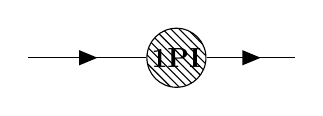
\begin{tikzpicture}[baseline = -0.11cm]
\begin{feynman}
\vertex (a);
\vertex [right=of a, blob] (b) {\(\mathbf{1PI}\)};
\vertex [right=of b] (f1);
\diagram* {
(a) -- [fermion] (b) -- [fermion] (f1)
};
\end{feynman}
\end{tikzpicture}
 = - i \Sigma(p^2)
\end{equation*}
represent the sum of all one-particle irreducible diagrams to the order of perturbation theory we are working in. We will call the amplitude for the total one-particle irreducible diagrams $-i \Sigma(p^2)$. Then, the total dressed propagator is given diagrammatically (dropping the first order line) as the sum,
\begin{equation*}
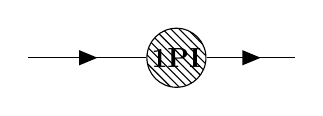
\begin{tikzpicture}[baseline = -0.11cm]
\begin{feynman}
\vertex (a);
\vertex [right=of a, blob] (b) {\(\mathbf{1PI}\)};
\vertex [right=of b] (c);
\diagram* {
(a) -- [fermion] (b) -- [fermion] (c)
};
\end{feynman}
\end{tikzpicture}
\quad
\mathlarger{+}
\quad 
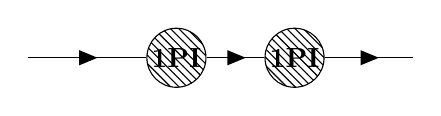
\begin{tikzpicture}[baseline = -0.11cm]
\begin{feynman}
\vertex (a);
\vertex [right=of a, blob] (b) {\(\mathbf{1PI}\)};
\vertex [right=of b, blob] (c) {\(\mathbf{1PI}\)};
\vertex [right=of c] (d);
\diagram* {
(a) -- [fermion] (b) -- [fermion] (c) -- [fermion] (d)
};
\end{feynman}
\end{tikzpicture}
\quad
\mathlarger{+}
\quad 
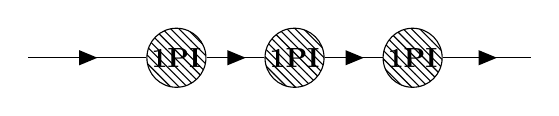
\begin{tikzpicture}[baseline = -0.11cm]
\begin{feynman}
\vertex (a);
\vertex [right=of a, blob] (b) {\(\mathbf{1PI}\)};
\vertex [right=of b, blob] (c) {\(\mathbf{1PI}\)};
\vertex [right=of c, blob] (d) {\(\mathbf{1PI}\)};
\vertex [right=of d] (e);
\diagram* {
(a) -- [fermion] (b) -- [fermion] (c) -- [fermion] (d) -- [fermion] (e)
};
\end{feynman}
\end{tikzpicture}
\quad
\mathlarger{+}
\quad \cdots
\end{equation*}
and in terms of amplitudes,
\begin{align*} 
\tilde{G}^{(2)}(p) & = \frac{i}{p^2 - m^2 + i \epsilon} + \frac{i}{p^2 - m^2 + i \epsilon} ( - i \Sigma) \frac{i}{p^2 - m^2 + i \epsilon} \\
& \quad \quad \quad +
 \frac{i}{p^2 - m^2 + i \epsilon} ( - i \Sigma) \frac{i}{p^2 - m^2 + i \epsilon}  ( - i \Sigma) \frac{i}{p^2 - m^2 + i \epsilon}  + \cdots 
\\
& = \frac{i}{p^2 - m^2 + i \epsilon} \cdot \frac{1}{1 - ( - i \Sigma) \frac{i}{p^2 - m^2 + i \epsilon}} = \frac{i}{p^2 - m^2 - \Sigma(p^2) + i \epsilon}
\end{align*}
Since $\Sigma$ is generically a function of $p^2$, we can rewrite this expression in the form,
\begin{align*}
\tilde{G}^{(2)}(p) & = \frac{i}{p^2 - m^2 - \Sigma(p^2 = m^2) - (p^2 - m^2) \deriv{\Sigma}{p^2} - \tfrac{1}{2} (p^2 - m^2)^2 \frac{\mathrm{d}^2 \Sigma}{(\mathrm{d} p^2)^2} + \cdots + i \epsilon}
\end{align*}
From the LSZ reduction formula, we know that the physical propagator must have a pole at the physical mass $m$. Therefore, we require the renormalization condition, 
\[\Sigma(p^2 = m^2) = 0\]
Thus, we can write,
\begin{align*}
\tilde{G}^{(2)}(p) & = \frac{i}{p^2 - m^2  - (p^2 - m^2) \deriv{\Sigma}{p^2} - \tfrac{1}{2} (p^2 - m^2)^2 \frac{\mathrm{d}^2 \Sigma}{(\mathrm{d} p^2)^2} + \cdots + i \epsilon}
\\
& = \frac{i}{p^2 - m^2 + i \epsilon} \cdot \frac{1}{1 - \deriv{\Sigma}{p^2} - \tfrac{1}{2} (p^2 - m^2) \frac{\mathrm{d}^2 \Sigma}{(\mathrm{d} p^2)^2} + \cdots }
\\
& = \frac{i \left(1 - \deriv{\Sigma}{p^2} \middle|_{p^2 = m^2} \right)^{-1}}{p^2 - m^2 + i \epsilon} + \frac{i}{p^2 - m^2 + i \epsilon} \left[ \frac{1}{1 - \deriv{\Sigma}{p^2} - \tfrac{1}{2} (p^2 - m^2) \frac{\mathrm{d}^2 \Sigma}{(\mathrm{d} p^2)^2} + \cdots } - \frac{1}{1 - \deriv{\Sigma}{p^2} } \right] 
\\
& = \frac{i \left(1 - \deriv{\Sigma}{p^2} \middle|_{p^2 = m^2} \right)^{-1}}{p^2 - m^2 + i \epsilon} + \frac{i}{p^2 - m^2 + i \epsilon} \left[ \frac{1 - \deriv{\Sigma}{p^2} - \left(1 - \deriv{\Sigma}{p^2} - \tfrac{1}{2} (p^2 - m^2) \frac{\mathrm{d}^2 \Sigma}{(\mathrm{d} p^2)^2} + \cdots \right)}{\left(1 - \deriv{\Sigma}{p^2} - \tfrac{1}{2} (p^2 - m^2) \frac{\mathrm{d}^2 \Sigma}{(\mathrm{d} p^2)^2} + \cdots \right) \cdot \left(1 - \deriv{\Sigma}{p^2} \right) } \right]
\\
& = \frac{i \left(1 - \deriv{\Sigma}{p^2} \middle|_{p^2 = m^2} \right)^{-1}}{p^2 - m^2 + i \epsilon} + i \left[ \frac{ \tfrac{1}{2} \frac{\mathrm{d}^2 \Sigma}{(\mathrm{d} p^2)^2} + \cdots}{\left(1 - \deriv{\Sigma}{p^2} - \tfrac{1}{2} (p^2 - m^2) \frac{\mathrm{d}^2 \Sigma}{(\mathrm{d} p^2)^2} + \cdots \right) \cdot \left(1 - \deriv{\Sigma}{p^2} \right) } \right]
\end{align*}
The second term is regular at $p^2 = m^2$ so this form of the dressed propagator exactly matches the form of the LSZ two-point function with a pole at the physical mass and a residue,
\[ Z = \left(1 - \deriv{\Sigma}{p^2} \middle|_{p^2 = m^2} \right)^{-1}\]

\subsection{The Dressed $\psi$ Propagator (b)}

It remains to actually calculate this factor $\Sigma(p^2)$. At the one-loop level, there are exactly two one-particle irreducible diagrams,
\begin{equation*}
\feynmandiagram [horizontal = a to b, layered layout, baseline = (a)] {
	i1 -- [fermion, momentum'=$p$] a -- [fermion, momentum'=$p - k$] b -- [fermion, momentum'=$p$] f1,
	a -- [scalar, half left, momentum=$k$] b
	};
\quad
\mathlarger{+}
\quad 	
\feynmandiagram [horizontal = a to b, layered layout, baseline = (a)] {
	i1 -- [fermion, momentum'=$p$] a [crossed dot, label = \(- i c_2\)] -- [fermion, momentum'=$p$] b
	};	
\end{equation*}
From the Feynman rules, the amplitude for these two terms is,
\[ - i \Sigma_\psi(p^2) = (-ig)^2 \int \frac{\mathrm{d}^4 k}{(2 \pi)^4} \frac{i}{k^2 - m^2 + i \epsilon} \cdot \frac{i}{(p - k)^2 - M^2 + i \epsilon} - i c_2 \]
\subsection{Calculating The $\psi$ Loop Integral (c)}
Now it is time to evaluate this nasty integral,
\[ V(p) = \int \frac{\mathrm{d}^4 k}{(2 \pi)^4} \frac{i}{k^2 - m^2 + i \epsilon} \cdot \frac{i}{(p - k)^2 - M^2 + i \epsilon} \]
First, introduce Feynman parameters via the identity,
\[ \frac{1}{AB} = \int_0^1 \frac{\delta(x+y-1)}{(xA + y B)^2} \: \d{x}\d{y} \] 
Therefore,
\[ V(p) = \int_{0}^{1} \d{x} \d{y} \int \frac{\mathrm{d}^4 k}{(2\pi)^4} \cdot \frac{-\delta(x + y - 1)}{\left[k^2 - 2 y p \cdot k + y p^2 - m^2 x - M^2 y + i \epsilon \right]^2}\]
completing the square,
\[ V(p) = \int_{0}^{1} \d{x} \d{y} \int \frac{\mathrm{d}^4 k}{(2\pi)^4} \cdot \frac{-\delta(x + y - 1)}{\left[(k - y p)^2 - y^2 p^2 + y p^2 - m^2 x - M^2 y + i \epsilon \right]^2}\]
Now we can shift the integration variables, $\ell = k - y p$ to get,
\[ V(p) = \int_{0}^{1} \d{x} \d{y} \int \frac{\mathrm{d}^4 \ell}{(2\pi)^4} \cdot \frac{-\delta(x + y - 1)}{\left[\ell^2 - y^2 p^2 + y p^2 - m^2 x - M^2 y + i \epsilon \right]^2}\]
Next, we will perform a Wick rotation so that the integral can be evaluated in Euclidean space rather than Minkowski space. This transformation takes $\ell^0 = i \ell^0_E$. Therefore, 
\[ V(p) = i \int_{0}^{1} \d{x} \d{y} \int \frac{\mathrm{d}^4 \ell_E}{(2\pi)^4} \cdot \frac{-\delta(x + y - 1)}{\left[\ell_E^2 + y^2 p^2 - y p^2 + m^2 x + M^2 y - i \epsilon \right]^2}\]
Because this integral is spherically symmetric in four dimensional Euclidean space, we can integrate over angles first, 
\[ V(p) = 2 \pi^2 i \int_{0}^{1} \d{x} \d{y} \int_{0}^\infty \frac{\d{\ell_E}}{(2\pi)^4} \cdot \frac{ -\ell_E^3 \delta(x + y - 1)}{\left[\ell_E^2 + y^2 p^2 - y p^2 + m^2 x + M^2 y - i \epsilon \right]^2}\]
Now we use the Schwinger trick regularized with some parameter $\delta$, and calling,
\[\Delta = y^2 p^2 - y p^2 + m^2 x + M^2 y - i \epsilon\]
we get,
\begin{align*}
V(p) & = -2 \pi^2 i \int_{0}^{1} \d{x} \d{y} \delta(x + y - 1) \int_{0}^\infty \frac{\ell_E^3 \: \d{\ell_E} }{(2\pi)^4} \int_{\delta}^\infty \frac{\d{s}}{s} s^2 e^{ - s \left[  \ell_E^2 + \Delta \right] } 
\\
& = -\frac{i}{8 \pi^2} \int_{0}^{1} \d{x} \d{y} \delta(x + y - 1) \int_{\delta}^\infty \frac{\d{s}}{s} s^2 e^{ - s \Delta } \int_{0}^\infty \d{\ell_E} \: \ell_E^3 e^{-s \ell_E^2} 
\end{align*} 
Now, using the fact that,
\[ \int_0^\infty x^3 \: e^{-s x^2} \d{x} = \frac{1}{2 s^2} \]
we get,
\begin{align*}
V(p) & = -\frac{i}{16 \pi^2} \int_{0}^{1} \d{x} \d{y} \delta(x + y - 1) \int_{\delta}^\infty \frac{\d{s}}{s} e^{ - s \Delta } \xrightarrow{\delta \to 0} \frac{i}{16 \pi^2} \int_{0}^{1} \d{x} \d{y}  \delta(x + y - 1) \left[ \gamma_E + \log{\delta} + \log{\Delta} \right]
\end{align*} 
Writing the entire one-particle irreducible term in its full glory,
\[ - i \Sigma_\psi(p^2) = (-ig)^2 V(p) - i c_2 = -\frac{ig^2}{16 \pi^2} \left[\gamma_E + \log{\delta} + \int_{0}^{1} \d{x} \log{\left[ x(x - 1) p^2 + x m^2 + (1 - x) M^2 - i \epsilon \right]} \right] - i c_2 \]
For $p^2 = 0$, this integral is now perfectly finite and without poles in $x, y$ we can take $\epsilon \to 0$. The renormalization condition requires that $\Sigma_\psi(p^2 = M^2) = 0$ so we fix,
\[ c_2 = -\frac{g^2}{16 \pi^2} \left[ \gamma_E + \log{\delta} + \int_{0}^{1} \d{x}   \log{\left[ x m^2 + (x - 1)^2 M^2 \right]} \right] \]
The argument of the logarithm is manifestly positive so there is no danger that our counterterm becomes complex. This is good because having a complex counterterm in the Hamiltonian would break its Hermiticity which we have been assuming holds.
Finally,
\[ - i \Sigma_\psi(p^2) = (-ig)^2 V(p) - i c_2 = -\frac{ig^2}{16 \pi^2} \left[ \int_{0}^{1} \d{x} \log{\left[\frac{ x(x - 1) p^2 + x m^2 + (1 - x) M^2}{x m^2 + (x - 1)^2 M^2} \right]} \right] \]
which is nice and well-defined. To find the residue $Z_\psi$ we need to take the derivative of this quantity with respect to $p^2$. We get,
\[ \deriv{\Sigma_\psi}{p^2} = \frac{g^2}{16 \pi^2} \left[ \int_{0}^{1} \d{x} \frac{x(x - 1)}{ x(x - 1) p^2 + x m^2 + (1 - x) M^2} \right] \] 
The residue is then given by,
\[ Z_\psi = \left(1 - \deriv{\Sigma}{p^2} \middle|_{p^2 = M^2} \right)^{-1}\]
and thus,
\[ Z_\psi = \left(1 -  \frac{g^2}{16 \pi^2} \left[ \int_{0}^{1} \d{x} \frac{x(x - 1)}{ x m^2 + (x - 1)^2 M^2} \right] \right)^{-1}\]
We will save the calculation of explicit forms for these integral until the end of the section.
 
\subsection{Dimensional Regularization of the $\psi$ Loop Integral (d)}

This integral may be reevaluated by dimensional regularization. Start from the step following the Wick rotation, replacing the four dimensional integral with a $D = 4 - \delta$ dimensional integral, and evaluate in $D$-dimensional spherical coordinates,
\[ V(p) = -i \int_{0}^{1} \d{x} \d{y} \int \frac{\mathrm{d}^{D} \ell_E}{(2\pi)^D} \cdot \frac{\delta(x + y - 1)}{\left[\ell_E^2 + \Delta \right]^2} = \frac{2i \pi^{D/2}}{\Gamma \left(\frac{D}{2}\right)} \int_{0}^{1} \d{x} \d{y} \int \frac{\d{\ell_E} \: \ell_E^{D-1}}{(2\pi)^D} \cdot \frac{\delta(x + y - 1)}{\left[\ell_E^2 + \Delta \right]^2} \]
Now, introducing a a Schwinger parameter,
\begin{align*}
V(p) & = -\frac{2i}{(4 \pi)^{D/2} \Gamma \left(\frac{D}{2}\right)} \int_{0}^{1} \d{x} \d{y} \delta(x + y - 1) \int_0^\infty \d{\ell_E} \: \ell_E^{D-1} \int_0^\infty \frac{\d{s}}{s} \: s^2 \: e^{-s (\ell_E^2 + \Delta)} 
\\
& = -\frac{2i}{(4 \pi)^{D/2} \Gamma \left(\frac{D}{2}\right)} \int_{0}^{1} \d{x} \d{y} \delta(x + y - 1) \int_0^\infty \frac{\d{s}}{s} \: s^2 \: e^{- s \Delta} \int_0^\infty \d{\ell_E} \: \ell_E^{D-1}  \: e^{-s \: \ell_E^2} 
\end{align*}
Now, consider the integral and the substitution, $u = s x^2$, 
\begin{align*}
\int_0^\infty \d{x} \: x^{D-1} \: e^{-s x^2} = \frac{1}{2s} \int_{0}^\infty \d{u} \: (u/s)^{(D-2)/2} e^{-u} = \frac{1}{2 s^{D/2}} \Gamma\left(\tfrac{D}{2}\right)  
\end{align*}
Plugging into our integral,
\begin{align*}
V(p) & = - \frac{i}{(4 \pi)^{D/2}} \int_{0}^{1} \d{x} \d{y} \delta(x + y - 1) \int_0^\infty \frac{\d{s}}{s} s^{2 - D/2} e^{-s \Delta}
\\
& = -\frac{i}{16 \pi^{D/2}} \Gamma\left(2 - \frac{D}{2} \right) \int_{0}^{1} \d{x} \d{y} \delta(x + y - 1) \Delta^{D/2 - 2} 
\\
& = - \frac{i}{(4 \pi)^2} \int_{0}^{1} \d{x} \d{y} \delta(x + y - 1) \Gamma\left(\tfrac{\delta}{2}\right) \left[(4 \pi)^{-1} \Delta \right]^{- \delta / 2}
\end{align*}
Now, we use the fact that,
\[ \Gamma\left(\tfrac{\delta}{2}\right) = \frac{2}{\delta} - \gamma_E + O(\delta) \]
and that,
\[ \lim\limits_{\delta \to 0} \frac{1 - Q^{-\delta/2}}{\delta/2} =  \lim\limits_{\delta \to 0} \int_1^Q x^{-\delta/2 - 1} \: \d{x} = \int_1^Q \lim\limits_{\delta \to 0^-} x^{-\delta/2 - 1} \: \d{x}  = \int_1^Q \lim\limits_{\delta \to 0} x^{- 1} \: \d{x} = \log{Q} \]
Therefore, to order below $O(\delta)$,
\begin{align*} 
\Gamma\left(\tfrac{\delta}{2}\right) \left[(4 \pi)^{-1} \Delta \right]^{- \delta / 2}
& = \frac{2}{\delta} \: \left[(4 \pi)^{-1} \Delta \right]^{- \delta / 2} - \gamma_E \Delta^{- \delta / 2} + O(\delta) = \frac{\Delta^{-\delta/2} - 1}{\delta/2} + \frac{2}{\delta} - \gamma_E \left[(4 \pi)^{-1} \Delta \right]^{- \delta / 2} + O(\delta)
\\
&  \xrightarrow{\delta \to 0} \frac{2}{\delta} - \log{(4 \pi)^{-1} \Delta} - \gamma_E  + O(\delta) = \frac{2}{\delta} - \log{\Delta} - \gamma_E + \log{4 \pi} + O(\delta)
\end{align*}
Our final answer is that,
\begin{align*}
 V(p) = -\frac{i}{(4 \pi)^2} \left[ \frac{2}{\delta} - \gamma_E + \log{4 \pi} + O(\delta) -  \int_{0}^{1} \d{x} \d{y} \delta(x + y - 1) \log{\Delta} \right]
\end{align*}
Again writing the entire one-particle irreducible term in its full glory,
\[ - i \Sigma_\psi(p^2) = (-ig)^2 V(p) - i c_2 = -\frac{ig^2}{16 \pi^2} \left[ - \frac{2}{\delta} + \gamma_E - \log{4 \pi} + \int_{0}^{1} \d{x} \log{\left[ x(x - 1) p^2 + x m^2 + (1 - x) M^2 \right]} \right] - i c_2 \]
Up to constants and the form of the divergence which will both be renormalized away, this integral is exactly what we had before. 
The renormalization condition requires that $\Sigma_\psi(p^2 = M^2) = 0$ so we fix,
\[ c_2 = -\frac{g^2}{16 \pi^2} \left[ - \frac{2}{\delta} + \gamma_E - \log{4 \pi} + \int_{0}^{1} \d{x}   \log{\left[ x m^2 + (x - 1)^2 M^2 \right]} \right] \]
The argument inside the log is manifestly positive so the integral is real. This means the counterterm is real which must be true since the counter term appears in the Hamiltonian which is required to be a Hermitian operator. Finally,
\[ - i \Sigma_\psi(p^2) = (-ig)^2 V(p) - i c_2 = - \frac{ig^2}{16 \pi^2} \left[ \int_{0}^{1} \d{x} \log{\left[\frac{ x(x - 1) p^2 + x m^2 + (1 - x) M^2}{x m^2 + (x - 1)^2 M^2} \right]} \right] \]
which is nice and well-defined and thankfully the same as what we calculated before.

\subsection{The Dressed $\phi$ Propagator (e)}

Now we must renormalize the $\phi$ propagator. Our calculation of the dressed propagator is entirely general so we must simply calculate the one-particle irreducible amplitude on a $\phi$ propagator line. At the one-loop level, there are exactly two diagrams which contribute,
\begin{equation*}
\feynmandiagram [horizontal = a to b, layered layout, baseline = (a)] {
	i1 -- [scalar, momentum'=$p$] a -- [fermion, half right, momentum'=$p + k$] b -- [scalar, momentum'=$p$] f1,
	b -- [fermion, half right, momentum'=$k$] a
	};
\quad
\mathlarger{+}
\quad 	
\feynmandiagram [horizontal = a to b, layered layout, baseline = (a)] {
	i1 -- [scalar, momentum'=$p$] a [crossed dot, label = \(- i c_3\)] -- [scalar, momentum'=$p$] b
	};	
\end{equation*} 
From the Feynman rules, the amplitude for these two terms is,
\[ - i \Sigma_\phi(p^2) = (-ig)^2 \int \frac{\mathrm{d}^4 k}{(2 \pi)^4} \frac{i}{k^2 - M^2 + i \epsilon} \cdot \frac{i}{(p + k)^2 - M^2 + i \epsilon} - i c_3 \]
We need to evaluate this nasty integral,
\[ V(p) = \int \frac{\mathrm{d}^4 k}{(2 \pi)^4} \frac{i}{k^2 - m^2 + i \epsilon} \cdot \frac{i}{(p + k)^2 - M^2 + i \epsilon} \]
but luckily this integral is nearly identical to the one we computed before in painstaking detail. The only changes are $p \to -p$ (which changes nothing) and take $m \to M$. Therefore, using the Schwinger regularization,
\[ V(p) = \frac{i}{16 \pi^2}  \left[ \gamma_E + \log{\delta} +  \int_{0}^{1} \d{x} \log{\left[ x(x-1)p^2 + M^2 \right]} \right] \]
Therefore, the one-particle irreducible part becomes,
\[ - i \Sigma_\phi(p^2) = - \frac{ig^2}{16 \pi^2}  \left[ \gamma_E + \log{\delta} + \int_{0}^{1} \d{x} \log{\left[ x(x-1)p^2 + M^2 \right]} \right] - i c_3 \]
The renormalization condition requires that $\Sigma_\phi(p^2 = m^2) = 0$ so we fix,
\[ c_3 = - \frac{g^2}{16 \pi^2} \left[ \gamma_E + \log{\delta} + \int_{0}^{1} \d{x}   \log{\left[ x(x - 1) m^2 + M^2 \right]} \right] \]
Finally,
\[ - i \Sigma_\phi(p^2) = (-ig)^2 V(p) - i c_3 = - \frac{ig^2}{16 \pi^2} \left[ \int_{0}^{1} \d{x} \log{\left[\frac{x(x - 1) p^2 + M^2}{x(x - 1) m^2 + M^2} \right]} \right] \]
which is nice and well-defined. To find the residue $Z_\phi$ we need to take the derivative of this quantity with respect to $p^2$. We get,
\[ \deriv{\Sigma_\phi}{p^2} = \frac{g^2}{16 \pi^2} \left[ \int_{0}^{1} \d{x}\frac{x(x - 1)}{ x(x - 1) p^2 + M^2} \right] \] 
The residue is then given by,
\[ Z_\phi = \left(1 - \deriv{\Sigma}{p^2} \middle|_{p^2 = m^2} \right)^{-1}\]
and thus,
\[ Z_\phi = \left(1 - \frac{g^2}{16 \pi^2} \left[ \int_{0}^{1} \d{x}  \frac{x(x - 1)}{ x(x - 1) m^2 + M^2} \right] \right)^{-1}\]
However, I have made an oversight in this calculation. We require that the counterterms be real such that the Lagrangian and thus the Hamiltonian remain real. Therefore, if the one-particle irreducible amplitude $\Sigma_\phi$ is complex, there is no way it can be entirely canceled by a real counterterm. In this case, we instead require, $\mathrm{Re}[\Sigma_\phi(p^2 = m^2)] = 0$ such that the location of the propagator peak for real momentum is unchanged but the propagator may pick up a finite imaginary part at $p^2 = m^2$. The field strength is defined as, 
\[Z = |\bra{\Omega}\phi(0)\ket{\lambda_0}|^2\]
which is a manifestly positive real quantity. Therefore, extra care must be when calculating the residue of an unstable particle. Consider the form of the two-point function,
\[ \tilde{G}^{(2)}(p) = \frac{i Z}{p^2 - m^2 + i m \Gamma(p)} \]
If we compare this to the result obtained by summing one-particle irreducible diagrams,
\begin{align*}
\tilde{G}^{(2)}(p) & = \frac{i}{p^2 - m^2 - \mathrm{Re}[\Sigma(p^2)] - i \mathrm{Im}[\Sigma(p^2)]}
\\
& = \frac{i}{p^2 - m^2 - (p^2 - m^2) \deriv{\mathrm{Re}[\Sigma]}{p^2}  - i \mathrm{Im}[\Sigma(p^2)]} + f(p^2) =\frac{i Z}{p^2 - m^2 - i Z \mathrm{Im}[\Sigma(m^2)]} + f(p^2) 
\end{align*}
where,
\[ Z = \left(1 - \deriv{\mathrm{Re}[\Sigma]}{p^2} \bigg|_{p^2 = m^2} \right) \]
If the resonance is narrow, we can approximate the value of the imaginary part by its value at $m^2$ over the width of the resonance,
\[ G^{(2)}_\phi(p) \approx \frac{i}{p^2 - m^2 - \Sigma_\phi(p^2)} = \frac{i Z}{p^2 - m^2 + i m \Gamma_\phi} + f(p^2)\]
where $f(p^2)$ is regular at $p^2 = m^2$ and $\Sigma(p^2 = m^2) = -\frac{1}{Z} i m \Gamma$. This is a relativistic form of the Breit-Wigner distribution representing an unstable particle. If we look back at our formula for $-i \Sigma_\phi(p^2)$,
\[ - i \Sigma_\phi(p^2) = - \frac{ig^2}{16 \pi^2}  \left[ \gamma_E + \log{\delta} + \int_{0}^{1} \d{x} \log{\left[ x(x-1)p^2 + M^2 - i \epsilon \right]} \right] - i c_3 \]
we see that if the argument of the logarithm is negative then the integral will give an imaginary value which cannot be canceled by the counterterm. Looking at the term,
\[ \Sigma_\phi(p^2) = \frac{g^2}{16 \pi^2}  \left[ \gamma_E + \log{\delta} + \int_{0}^{1} \d{x} \log{\left[ x(x-1)p^2 + M^2 - i \epsilon \right]} \right] + c_3 \]
we see that,
\[\Im[\Sigma_\phi(p^2)] = \frac{g^2}{16 \pi^2} \mathrm{Im}\left[ \int_{0}^{1} \d{x} \log{\left[ x(x-1)p^2 + M^2 \right]} \right] \] 
Therefore, we should consider the term inside the logarithm at $p^2 = m^2$ with some care. Completing the square,
\[ x(x-1) m^2 + M^2 = x^2 m^2 - x m^2 + M^2 = (mx - \tfrac{1}{2}m)^2 - \tfrac{1}{4} m^2 + M^2 \]
Thus, this term will be strictly positive only when $M^2 > \tfrac{1}{4} m^2$ or equivalently, $m < 2 M$. Using the identity,
\[ \mathrm{Im}\left[ \log{(x - i \epsilon)} \right] = - \pi \theta(-x) \]
we can explicitly evaluate this integral,
\begin{align*}
\mathrm{Im}\left[ \int_{0}^{1} \d{x} \log{\left[ x(x-1)p^2 + M^2 - i \epsilon \right]} \right] & = \int_{0}^{1} \d{x} \mathrm{Im}\left[ \log{\left[ x(x-1)m^2 + M^2 - i \epsilon \right]} \right] 
\\
& = - \pi \int_{0}^{1} \d{x} \theta(x(1-x) m^2 - M^2)  = - \pi \int_{r_1}^{r_2} \d{x} = - i \pi (r_2 - r_1)
\end{align*} 
where $r_1 < r_2$ are the (real) roots of the quadratic $m^2 x^2 - m^2 x + M^2 = 0$. From the quadratic formula, 
\[ r_{\pm} = \frac{m^2 \pm \sqrt{m^4 - 4 m^2 M^2}}{2 m^2} = \frac{1}{2} \pm \sqrt{\frac{1}{4} - \frac{M^2}{m^2}} \quad \text{so} \quad r_2 - r_1 = \sqrt{1 - \frac{4 M^2}{m^2}} \]
Therefore,
\begin{align*}
\Im[\Sigma_\phi(p^2)] = \frac{g^2}{16 \pi^2}\mathrm{Im}\left[ \int_{0}^{1} \d{x} \log{\left[ x(x-1)m^2 + M^2 - i \epsilon \right]} \right] & = 
-\frac{g^2}{16 \pi}
\begin{cases}
\sqrt{1 - \frac{4M^2}{m^2}} & m > 2M \\
0 & m \le 2M
\end{cases}
\end{align*}
We see explicitly that $\Sigma_\phi(p^2 = m^2)$ becomes complex exactly when $m > 2 M$. When we have $m > 2 M$ and thus the meson becomes unstable, the Breit-Wigner width is given by,
\[ \Gamma_\phi = - \frac{Z_\phi}{m} \mathrm{Im}[ \Sigma_\phi(p^2 = m^2) ] =  \frac{Z_\phi g^2}{16 \pi m} \sqrt{1 - \frac{4M^2}{m^2}} \]
which is an invariant measure of the inverse meson lifetime. \bigskip\\
Since these integrals are going to play a large role in the scattering amplitude, we ought to evaluate them exactly in full generality. This will require some casework.

\subsection{Explicit Computations of the One-Particle Irreducible Amplitudes}
In this section we will explicitly evaluate integrals of some complex functions which show up in the calculation of the one-part irreducible amplitude. 
\subsubsection{Evaluation of the $\phi$ One-Particle Irreducible Amplitude in the Case $m < 2 M$}

First, we restrict to the case $m < 2 M$ in which the $\phi$ meson is stable and thus asymptotic scattering $\phi$ states can be defined. For $0 < p^2 < 4 M^2$ the argument of the integral,
\[ - i \Sigma_\phi(p^2) = (-ig)^2 V(p) - i c_3 = - \frac{ig^2}{16 \pi^2} \left[ \int_{0}^{1} \d{x} \log{\left[\frac{x(x - 1) p^2 + M^2}{x(x - 1) m^2 + M^2} \right]} \right] \]
is everywhere positive. In this case, Mathematica has no issue evaluating this integral, 
\begin{align*}
- i \Sigma_\phi(p^2) &= - \frac{ig^2}{16 \pi^2} \left[ \int_{0}^{1} \d{x} \log{\left[\frac{x(x - 1) p^2 + M^2}{x(x - 1) m^2 + M^2} \right]} \right] 
\\
& = - \frac{ig^2}{8 \pi^2} \left[ \sqrt{\frac{4 M^2 - p^2}{p^2}} \arctan{\left( \sqrt{\frac{p^2}{4 M^2 - p^2}} \right)} - \sqrt{\frac{4 M^2 - m^2}{m^2}} \arctan{\left( \sqrt{\frac{m^2}{4 M^2 - m^2}}\right)}\right]
\end{align*}
Since the factor $x(x-1) < 0$, in the case $p^2 < 0$ the argument of the logarithm remains positive. This ensures that $\Sigma_\phi$ will still be real in this region. We can obtain its value either by analytically extending the arc-tangent function to imaginary values or by having Mathematica evaluate the integral for negative $p^2$. Either way, when $p^2 < 0$ we get,
\begin{align*}
- i \Sigma_\phi(p^2) &= - \frac{ig^2}{16 \pi^2} \left[ \int_{0}^{1} \d{x} \log{\left[\frac{x(1 - x) p^2 + M^2}{x(x - 1) m^2 + M^2} \right]} \right] 
\\
& = - \frac{ig^2}{8 \pi^2} \left[ \sqrt{\frac{4 M^2 - p^2}{-p^2}} \mathrm{arctanh}{\left(\sqrt{\frac{-p^2}{4 M^2 - p^2}}\right)} - \sqrt{\frac{4 M^2 - m^2}{m^2}} \arctan{\left(\sqrt{\frac{m^2}{4 M^2 - m^2}}\right)}\right]
\end{align*}
The last case is when $p^2 > 4 M^2$. In this case, the momentum passes through the $\phi$ mesons creation resonance at which point the numerator becomes imaginary so the integral picks up an imaginary part. We can get the real part of $\Sigma$ by analytically extending our first result past $p^2 = 4 M^2$ using the fact that,
\[ \mathrm{Re}[\log{(-x)}] = \log{(x)} \]
By analytic extension, in the region $p^2  > 4 M^2$, the term,
\[\sqrt{\frac{4 M^2 - p^2}{p^2}} \arctan{\left(\sqrt{\frac{p^2}{4 M^2 - p^2}}\right)} \to \sqrt{\frac{p^2 - 4 M^2}{p^2}} \mathrm{arctanh}{\left(\sqrt{\frac{p^2}{p^2 - 4 M^2}}\right)} = \frac{1}{2} \sqrt{\frac{4 M^2 - p^2}{p^2}} \log{\left[ \frac{1 + \sqrt{\frac{p^2}{p^2 - 4 M^2}}}{1 - \sqrt{\frac{p^2}{p^2 - 4 M^2}}} \right]}\]
However, the square root factor inside the log is greater than one so the argument of the log is negative. Therefore, using the above identity, the real part becomes,
\[\sqrt{\frac{4 M^2 - p^2}{p^2}} \arctan{\left(\sqrt{\frac{p^2}{4 M^2 - p^2}}\right)} \to \frac{1}{2} \sqrt{\frac{4 M^2 - p^2}{p^2}} \log{\left[ \frac{\sqrt{\frac{p^2}{p^2 - 4 M^2}} + 1}{\sqrt{\frac{p^2}{p^2 - 4 M^2}} - 1} \right]}\]
To get the correct imaginary part, we must remember the factor of $-i \epsilon$ to integrate on the correct side of the branch cut. Using the same trick as before,  
\[ \mathrm{Im} \left[ \int_{0}^{1} \d{x} \log{\left[\frac{x(1 - x) p^2 + M^2 - i \epsilon}{x(x - 1) m^2 + M^2} \right]} \right]  = \int_{0}^{1} \d{x} \mathrm{Im}[\log{[x(1 - x) p^2 + M^2 - i \epsilon]}] = - \pi \sqrt{1 - \frac{4 M^2}{p^2}} \]
Therefore, in the region $p^2 > 4 M^2$ the full expression for the one-particle irreducible amplitude becomes,
\begin{align*}
- i \Sigma_\phi(p^2) 
& = - \frac{ig^2}{16 \pi^2} \left[ \sqrt{\frac{p^2 - 4 M^2}{p^2}} \log{\left[ \frac{\sqrt{\frac{p^2}{p^2 - 4 M^2}} + 1}{\sqrt{\frac{p^2}{p^2 - 4 M^2}} - 1} \right]} - 2 \sqrt{\frac{4 M^2 - m^2}{m^2}} \arctan{\left(\sqrt{\frac{m^2}{4 M^2 - m^2}}\right)} - \pi i \sqrt{1 - \frac{4 M^2}{p^2}} \right]
\end{align*}
Furthermore, in the case $m < 2M$ we can calculate the derivative which appears in the residue $Z_\phi$ using Mathematica since the integrand does not pass through a pole,
\[ \deriv{\Sigma_\phi}{p^2} = \frac{g^2}{16 \pi^2} \int_{0}^1 \d{x} \frac{x(x-1)}{x(x-1)m^2 + M^2} 
=
\frac{g^2}{16 \pi^2} \frac{1}{m^3} \left[ m - \frac{4 M^2}{\sqrt{4 M^2 - m^2}} \arctan{\left( \sqrt{\frac{m^2}{4 M^2 - m^2}} \right)} \right] \]
Therefore, the residue in the dressed $\phi$ propagator can be written,
\[ Z_\phi = \left( 1 - \frac{g^2}{16 \pi^2 m^2} + \frac{g^2}{16 \pi^2 m^3} \left[ \frac{4 M^2}{\sqrt{4 M^2 - m^2}} \arctan{\left( \sqrt{\frac{m^2}{4 M^2 - m^2}} \right)} \right]  \right)^{-1} \]
For future use, I will here define the field strength renormalized one-particle irreducible amplitude,
\begin{align*}
\Sigma_\phi^{renorm}(p^2) & = \Sigma_\phi(p^2) - (p^2 - m^2) \deriv{\Sigma_\phi}{p^2} \bigg|_{p^2 = m^2} 
\\
& = 
\frac{g^2}{16 \pi^2}
\begin{cases}
2 \sqrt{\frac{4 M^2 - p^2}{-p^2}} \mathrm{arctanh}{\left(\sqrt{\frac{-p^2}{4 M^2 - p^2}}\right)} 
& p^2 < 0
\\
&
\\
2 \sqrt{\frac{4 M^2 - p^2}{p^2}} \arctan{\left( \sqrt{\frac{p^2}{4 M^2 - p^2}} \right)} 
& 0 < p^2 < 4 M^2 
\\
&
\\
\sqrt{\frac{p^2 - 4 M^2}{p^2}} \log{\left[ \frac{\sqrt{\frac{p^2}{p^2 - 4 M^2}} + 1}{\sqrt{\frac{p^2}{p^2 - 4 M^2}} - 1} \right]}  - i \pi \sqrt{1 - \frac{4 M^2}{p^2}}
& p^2 > 4 M^2
\end{cases}
\\ 
& \quad \quad \quad 
- 2 \sqrt{\frac{4 M^2 - m^2}{m^2}} \arctan{\left(\sqrt{\frac{m^2}{4 M^2 - m^2}}\right)}
- \frac{p^2 - m^2}{m^3} \left[ m - \frac{4 M^2}{\sqrt{4 M^2 - m^2}} \arctan{\left( \sqrt{\frac{m^2}{4 M^2 - m^2}} \right)} \right]
\end{align*}

An important feature of this functional form is that $\Sigma_\phi(p^2)$ is real for $p^2 < (2 M)^2$ and $\Sigma_\phi(p^2)$ is complex for $p^2 > (2 M)^2$. Physically, this corresponds exactly to then energy needed to produce a two particle $\psi \bar{\psi}$ state. If $\Sigma_\phi(p^2)$ is viewed as a function of a complex variable then it has a branch cut starting at $p^2 = (2 M)^2$ due to the sign dependence of the imaginary part under the change $i \epsilon \to - i \epsilon$ in the integral. This branch cut corresponds to the mulitparticle continuum predicted by the K{\"a}ll{\'e}n-Lehmann spectral representation. However, in the case $m < M$ the multiparticle continuum should begin at $p^2 = (2 m)^2 < (2 M)^2$ since no conservation laws prohibit an off-shell $\phi \to \phi \phi$ process. However, this process enters the perturbative expansion of the two-point function with the diagram
\begin{center}
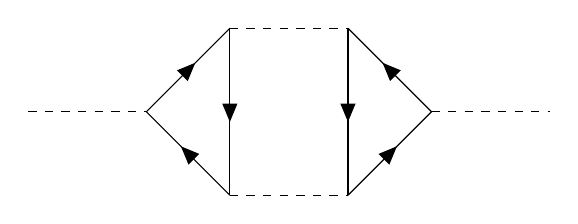
\begin{tikzpicture}
\begin{feynman}
\vertex (a);
\vertex[right=of a] (b);
\vertex[above right=of b] (l1);
\vertex[below right=of b] (l2);
\vertex[right=of l1] (l3);
\vertex[right=of l2] (l4);
\vertex[above right=of l4] (c);
\vertex[right=of c] (d);
\diagram* {
(a) -- [scalar] (b),
(b) -- [fermion] (l1) -- [fermion] (l2) -- [fermion] (b),
(l1) -- [scalar] (l3),
(l2) -- [scalar] (l4),
(c) -- [fermion] (l3) -- [fermion] (l4) -- [fermion] (c),
(c) -- [scalar] (d)
};
\end{feynman}
\end{tikzpicture}
\end{center}
at the three-loop level which is beyond the scope of our analysis. Therefore, a higher loop-order calculation would be necessary to probe the full structure of the multiparticle part of the dressed $\tilde{G}_{\psi}(p)$ propagator.  


\subsubsection{Evaluation of the $\phi$ One-Particle Irreducible Amplitude in the Case $m \ge 2 M$}

Now, we consider to the case $m > 2 M$. In this case, the $\phi$ meson is stable and thus asymptotic scattering $\phi$ states cannot be defined. This does not affect the current theory because we are not consider $S$ matrix elements corresponding to asymptotic $\phi$ states. We need to consider term,
\[ - i \Sigma_\phi(p^2) = - \frac{ig^2}{16 \pi^2}  \left[ \gamma_E + \log{\delta} + \int_{0}^{1} \d{x} \log{\left[ x(x-1)p^2 + M^2 - i \epsilon \right]} \right] - i c_3 \]
With the renormalization condition $\mathrm{Re}[\Sigma(p^2 = m^2)] = 0$. We have shown that there is a residual imaginary part at $p^2 = m^2$ given by,
\[\Im[\Sigma_\phi(p^2)] = \frac{g^2}{16 \pi^2} \mathrm{Im}\left[ \int_{0}^{1} \d{x} \log{\left[ x(x-1)p^2 + M^2 - i \epsilon \right]} \right] = -\frac{g^2}{16 \pi}
\begin{cases}
\sqrt{1 - \frac{4M^2}{p^2}} & m > 2M \\
0 & m \le 2M
\end{cases} \]
To satisfy the renormalization condition, following the above results we set,
\begin{align*}
c_3 & = - \frac{g^2}{16 \pi^2} \left[ \gamma_E + \log{\delta} + \int_0^1 \mathrm{Re}\left[ \log(x(x-1) m^2 + M^2 - i \epsilon) \right] \right] 
\\
&= - \frac{g^2}{16 \pi^2} \left[ \gamma_E + \log{\delta} + \sqrt{\frac{m^2 - 4 M^2}{m^2}} \log{\left[ \frac{\sqrt{\frac{m^2}{m^2 - 4 M^2}} + 1}{\sqrt{\frac{m^2}{m^2 - 4 M^2}} - 1} \right]} + 2( \log{M} - 1) \right]
\end{align*}
Therefore, we are interested in the quantity,
\[ - i \Sigma_\phi(p^2) = (-ig)^2 V(p) - i c_3 = - \frac{ig^2}{16 \pi^2} \left[ \int_{0}^{1} \d{x} \log{\left[\frac{x(x - 1) p^2 + M^2}{M^2} \right]} - \sqrt{\frac{m^2 - 4 M^2}{m^2}} \log{\left[ \frac{\sqrt{\frac{m^2}{m^2 - 4 M^2}} + 1}{\sqrt{\frac{m^2}{m^2 - 4 M^2}} - 1} \right]} + 2 \right] \]
Luckily, this integral is nearly identical to the one worked out above so I will simply quote the result,
\begin{align*}
\Sigma_\phi(p^2) =
\frac{g^2}{16 \pi^2}
\begin{cases}
2 \sqrt{\frac{4 M^2 - p^2}{-p^2}} \mathrm{arctanh}{\left(\sqrt{\frac{-p^2}{4 M^2 - p^2}}\right)} - \sqrt{\frac{m^2 - 4 M^2}{m^2}} \log{\left[ \frac{\sqrt{\frac{m^2}{m^2 - 4 M^2}} + 1}{\sqrt{\frac{m^2}{m^2 - 4 M^2}} - 1} \right]} 
& p^2 < 0
\\
&
\\
2 \sqrt{\frac{4 M^2 - p^2}{p^2}} \arctan{\left( \sqrt{\frac{p^2}{4 M^2 - p^2}} \right)} - \sqrt{\frac{m^2 - 4 M^2}{m^2}} \log{\left[ \frac{\sqrt{\frac{m^2}{m^2 - 4 M^2}} + 1}{\sqrt{\frac{m^2}{m^2 - 4 M^2}} - 1} \right]}
& 0 < p^2 < 4 M^2 
\\
&
\\
\sqrt{\frac{p^2 - 4 M^2}{p^2}} \log{\left[ \frac{\sqrt{\frac{p^2}{p^2 - 4 M^2}} + 1}{\sqrt{\frac{p^2}{p^2 - 4 M^2}} - 1} \right]} 
- \sqrt{\frac{m^2 - 4 M^2}{m^2}} \log{\left[ \frac{\sqrt{\frac{m^2}{m^2 - 4 M^2}} + 1}{\sqrt{\frac{m^2}{m^2 - 4 M^2}} - 1} \right]} - i\pi \sqrt{1 - \frac{4 M^2}{p^2}}
& p^2 > 4 M^2
\end{cases}
\end{align*}
To calculate the residue, we need to find the derivative of the real part of $\Sigma_\phi$. We can take this derivative directly from the above formula in the region $p^2 > 4 M^2$ (since $m > 2 M$). We get,
\[ \deriv{\mathrm{Re}[\Sigma_\phi]}{p^2} = \frac{g^2 M^2}{8 \pi p^4} \sqrt{\frac{p^2}{p^2-4 M^2}} \log{\left[\frac{\sqrt{\frac{p^2}{p^2-4
   M^2}}+1}{\sqrt{\frac{p^2}{p^2-4 M^2}}-1}\right]} + \frac{g^2}{16 \pi p^2}  \]
Therefore, when $m > 2 M$, the residue in the dressed $\phi$ propagator can be written,
\[ Z_\phi = \left( 1 - \frac{g^2 M^2}{8 \pi m^4} \sqrt{\frac{m^2}{m^2-4 M^2}} \log{ \left[\frac{\sqrt{\frac{m^2}{m^2-4
   M^2}}+1}{\sqrt{\frac{m^2}{m^2-4 M^2}}-1}\right]} - \frac{g^2}{16 \pi m^2}  \right)^{-1} \]
As before, I will here define the field strength renormalized one-particle irreducible amplitude,
\begin{align*}
\Sigma_\phi^{renorm}(p^2) & = \Sigma_\phi(p^2) - (p^2 - m^2) \deriv{\mathrm{Re}[\Sigma_\phi]}{p^2} \bigg|_{p^2 = m^2} 
\end{align*}

\subsubsection{Discussion of the $\psi$ One-Particle Irreducible Amplitude}

For $\phi$ particles there is no need to separately consider cases for the form of the two-point function. For all values of the parameters, $\Sigma_\psi(p^2 = M^2)$ is real the renormalization conditions can exactly fix $\Sigma_\psi(p^2 = M^2) = 0$. Therefore, the two-point function takes the form of a dressed propagator which can be considered in the asymptotic limit,
\[ \tilde{G}_\psi^{(2)}(p) = \frac{i Z}{p^2 - m^2 + i \epsilon} \]
This fact can directly be seen from the form of the integral, 
\[ - i \Sigma_\psi(m^2) = -\frac{ig^2}{16 \pi^2} \left[ \gamma_E + \log{\delta} + \int_{0}^{1} \d{x} \log{\left[ x m^2 + (1 - x)^2 M^2 \right]} \right] - i c_2 \]
in which, having taken $\epsilon \to 0$, the argument of the logarithm is clearly positive. Physically, the fact that $\Sigma_\phi(p^2 = M^2)$ is real is a reflection of the fact that $\phi$ particles must be stable due to the conservation of Noether charge. Since $\psi$ particles are the lowest mass excitation carrying Noether charge, the conservation law precludes $\psi$ decays which would have to end with a state of higher mass violating the conservation of energy. \bigskip\\
Although they are horrendous, the integrals determining $\Sigma_\psi$ can actually be explicitly computed. Luckily, since the form of these integrals is better behaved, there are fewer cases to consider. However, we will not actually need these integrals to compute the scattering cross section at this order so I will omit these details. All the important features can be read off from the pole structure of the integral,
\[ - i \Sigma_\psi(p^2) = - \frac{ig^2}{16 \pi^2} \left[ \int_{0}^{1} \d{x} \log{\left[\frac{ x(x - 1) p^2 + x m^2 + (1 - x) M^2}{x m^2 + (x - 1)^2 M^2} \right]} \right] \]
As discussed above, the denominator (and equivalently the counterterm) is real because $x m^2 + (1 - x)^2 M^2 \ge 0$. Consider the numerator which is the quadratic,
\[Q(x) = x(x - 1) p^2 + x m^2 + (1-x)M^2 = x^2 p^2 + x (m^2 - M^2 - p^2) + M^2 \]
First consider the case when $p^2 < 0$. Consider the endpoints $Q(0) = M^2$ and $Q(1) = p^2 + m^2 - M^2 - p^2 + M^2 = m^2$. Since both $Q(0) > 0$ and $Q(1) > 0$ and the parabola is convex down for $p^2 < 0$ we know that $Q(x) > 0$ for $x \in [0,1]$. Therefore, when $p^2 < 0$ the logarithm is real so $\Sigma_\psi$ is real and has no discontinuities. Furthermore, consider the case $p^2 > 0$. The discriminant of $Q$ is,
\[ (m^2 - M^2 - p^2)^2 - 4 M^2 p^2 = (p^2 - m^2 - M^2)^2 - 4 m^2 M^2 \]
However, 
\[ (p^2 - m^2 - M^2)^2 < 4 m^2 M^2 \iff - 2 m M < p^2 - m^2 - M^2 < 2 m M\]
which is equivalent to $(m - M)^2 < p^2 < (m + M)^2$. Therefore, $Q$ has real roots exactly when\[p^2 \in [0, (m - M)^2] \cup [(m+M)^2, \infty]\]
The maximum of this quadratic occurs at,
\[x_{max} = \frac{p^2 - m^2 + M^2}{2 p^2}  = \frac{1}{2} + \frac{M^2 - m^2}{2 p^2}\]
For the case $p^2 \in [0, (m - M)^2]$ this value satisfies,
\[ \left(x_{max} - \frac{1}{2} \right)^2 = \left( \frac{M^2 - m^2}{2 p^2} \right)^2 \ge \left( \frac{M^2 - m^2}{2 (M - m)^2} \right)^2 = \frac{1}{4} \left( \frac{M + m}{M - m} \right)^2  \ge \frac{1}{4}\]
Therefore, $x_{max} \notin [0, 1]$. However, since $Q(0) > 0$ and $Q(1) > 0$ if $Q(x) < 0$ for some $x \in [0, 1]$ then there would have to be a critical point in the range $[0, 1]$ which we have shown does not exist. Furthermore, if $p^2 > (m + M)^2$ then, 
\[ \left(x_{max} - \frac{1}{2} \right)^2 = \left( \frac{M^2 - m^2}{2 p^2} \right)^2 \le \left( \frac{M^2 - m^2}{2 (M + m)^2} \right)^2 = \frac{1}{4} \left( \frac{M - m}{M + m} \right)^2  \le \frac{1}{4}\]
Therefore, $x_{min} \in [0, 1]$ and since we know that $Q$ has a real root but has positive end behavior we must have $Q(x_{max}) < 0$ and thus the integrand becomes complex in this case. \bigskip\\
In summary, for $p^2 < (m + M)^2$ the function $\Sigma_{\psi}$ is real. For $p^2 \ge (m + M)^2$, there is a branch cut in the logarithm and $\Sigma_\psi$ picks up a imaginary part. Physically, this corresponds exactly to then energy needed to produce a two particle $\psi \phi$ state which is the lowest energy multiparticle state with Noether charge $1$. If $\Sigma_\psi(p^2)$ is viewed as a function of a complex variable then it has a branch cut starting at $p^2 = (m + M)^2$ due to the sign dependence of the imaginary part under the change $i \epsilon \to - i \epsilon$ in the integral. This branch cut again exactly corresponds to the multiparticle continuum predicted by the K{\"a}ll{\'e}n-Lehmann spectral representation.

\section{Computing the Scattering Amplitudes}
\subsection{Vertex Renormalization}

Next, we must consider the renormalization of the coupling constant $g$ such that the total vertex function looks like the physical coupling constant at a renormalization point. I will choose to renormalize at zero momentum which seems the most natural. This renormalization, requires another counterterm,
\[ \lagrange_{ct} = c_0 - c_1 \phi - c_2 \dpsi \psi - \tfrac{1}{2} c_3 \phi^2  - c_4 \dpsi \psi \phi \] 
which represents the shift between the physical and bare coupling constants and introduces a new vertex,
\begin{equation*}
\begin{tikzpicture}[baseline = -0.1cm]
\begin{feynman}
\vertex [crossed dot] (a) {};
\vertex [below left=of a] (b);
\vertex [above left=of a] (c);
\vertex [right=of a] (d);
\diagram* {
(a) -- [fermion] (b),
(c) -- [fermion] (a),
(a) -- [scalar] (d)
};
\end{feynman}
\end{tikzpicture}
= - i c_4
\end{equation*} 
At the one loop level, there are only three diagrams which contribute to the vertex function,
\begin{equation*}
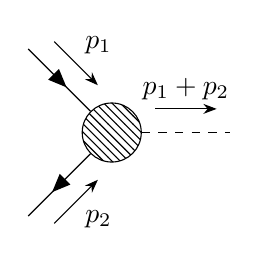
\begin{tikzpicture}[baseline = (b)]
\begin{feynman}
\vertex [blob] (b) {};
\vertex [above left=of b] (a);
\vertex [below left=of b] (c);
\vertex [right=of b] (d);
\diagram* {
(a) -- [fermion, momentum = $p_1$] (b) -- [fermion, rmomentum = $p_2$] (c),
(b) -- [scalar, momentum=$p_1 + p_2$] (d)
};
\end{feynman}
\end{tikzpicture}
 = - i \Gamma(p_1, p_2)
\end{equation*}

\begin{equation*}
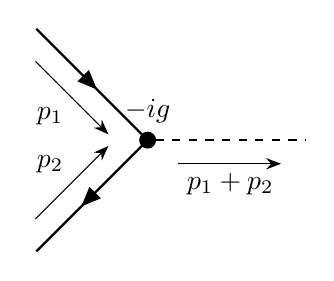
\begin{tikzpicture}[baseline = (a)]
\begin{feynman}[large]
\vertex [dot, label = $-ig$] (a) {};
\vertex [below left=of a] (b);
\vertex [above left=of a] (c);
\vertex [right=of a] (d);
\diagram* {
(a) -- [fermion, rmomentum'=$p_2$] (b),
(c) -- [fermion, momentum'=$p_1$] (a),
(a) -- [scalar, momentum'=$p_1 + p_2$] (d)
};
\end{feynman}
\end{tikzpicture}
\quad
\mathlarger{+}
\quad 	
\feynmandiagram [horizontal = a to b, baseline = (a)] {
	i1 -- [fermion, momentum'=$p_1$] t1 -- [fermion, momentum=$p_1 - k$] a,
	a -- [fermion, rmomentum=$p_2 + k$] t2 -- [fermion, rmomentum'=$p_2$] i2, 
	t1 -- [scalar, momentum'=$k$] t2,
	a -- [scalar, momentum'=$p_1 + p_2$ ] b
	};
\quad
\mathlarger{+}
\quad 	
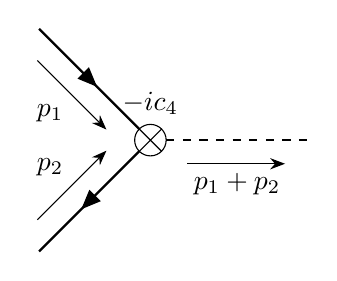
\begin{tikzpicture}[baseline = (a)]
\begin{feynman}[large]
\vertex [crossed dot, label = $-ic_4$] (a) {};
\vertex [below left=of a] (b);
\vertex [above left=of a] (c);
\vertex [right=of a] (d);
\diagram* {
(a) -- [fermion, rmomentum'=$p_2$] (b),
(c) -- [fermion, momentum'=$p_1$] (a),
(a) -- [scalar, momentum'=$p_1 + p_2$] (d)
};
\end{feynman}
\end{tikzpicture}
\end{equation*}
Using the Feynman rules,
\[ - i \Gamma(p_1, p_2) = (-ig) + (-ig)^3 \int \frac{\mathrm{d}^4 k}{(2 \pi)^4} \frac{i}{k^2 - m^2 + i \epsilon} \cdot \frac{i}{(p_1 - k)^2 - M^2 + i \epsilon} \cdot \frac{i}{(p_2 + k)^2 - M^2 + i \epsilon} - i c_4	\]
Therefore, we better evaluate this integral, 
\begin{align*}
V(p_1, p_2) =  \int \frac{\mathrm{d}^4 k}{(2 \pi)^4} \frac{i}{k^2 - m^2 + i \epsilon} \cdot \frac{i}{(p_1 - k)^2 - M^2 + i \epsilon} \cdot \frac{i}{(p_2 + k)^2 - M^2 + i \epsilon}
\end{align*}
Introducing Feynman parameters and remembering the factor of $(n-1)!$,
\begin{align*}
V(p_1, p_2) & = -2i \int \frac{\mathrm{d}^4 k}{(2 \pi)^4} \int_0^1 \frac{\d{x} \d{y} \d{z} \delta(x + y + z - 1)}{[x k^2 + y (p_1 - k)^2 + z (p_2 + k)^2 - x m^2 - (y + z) M^2 + i \epsilon]^3}
\\
& = -2i \int \frac{\mathrm{d}^4 k}{(2 \pi)^4} \int_0^1 \frac{\d{x} \d{y} \d{z} \delta(x + y + z - 1)}{[k^2 - 2 y p_1 \cdot k + y p_1^2 + 2 z p_2 \cdot k + z p_2^2 - x m^2 - (y + z) M^2 + i \epsilon]^3}
\\
& = -2i \int \frac{\mathrm{d}^4 k}{(2 \pi)^4} \int_0^1 \frac{\d{x} \d{y} \d{z} \delta(x + y + z - 1)}{[(k - yp_1 + z p_2)^2 - (y p_1 - z p_2)^2 + y p_1^2 + z p_2^2 - x m^2 - (y + z) M^2 + i \epsilon]^3}
\\
& = -2i \int \frac{\mathrm{d}^4 \ell}{(2 \pi)^4} \int_0^1 \frac{\d{x} \d{y} \d{z} \delta(x + y + z - 1)}{[\ell^2 - (y p_1 - z p_2)^2 + y p_1^2 + z p_2^2 - x m^2 - (y + z) M^2 + i \epsilon]^3}
\end{align*}
Now it is time to set $\Delta = (y p_1 - z p_2)^2 - y p_1^2 - z p_2^2 + x m^2 + (y + z) M^2 - i \epsilon$ and perform a Wick rotation $\ell^0 = i \ell_E^0$ so the integral becomes,
\begin{align*}
V(p_1, p_2) & = -2 \int \frac{\mathrm{d}^4 \ell_E}{(2 \pi)^4} \int_0^1 \frac{\d{x} \d{y} \d{z} \delta(x + y + z - 1)}{[\ell_E^2 + \Delta]^3}
\\
& = - \frac{4 \pi^2}{(2 \pi)^4} \int_0^1 \d{x} \d{y} \d{z} \delta(x + y + z - 1) \int_{0}^\infty \d{\ell_E} \frac{\ell_E^3}{[\ell_E^2 + \Delta]^3}
\end{align*}
However, 
\[ - \deriv{}{x} \frac{2 x^2 + \Delta}{4(x^2 + \Delta)^2} = -\frac{x}{(x^2 + \Delta)^2} + \frac{(2 x^2 + \Delta)x}{(x^2 + \Delta)^3} = \frac{x^3}{(x^2 + \Delta)^3}\]
Therefore, 
\[ \int_{0}^\infty \d{\ell_E} \frac{\ell_E^3}{[\ell_E^2 + \Delta]^3} = \left[ -\frac{2 x^2 + \Delta}{4(x^2 + \Delta)^2} \right]_{0}^\infty = \frac{1}{4 \Delta} \]
so the integral $V(p_1, p_2)$ is actually finite. At last,
\[ V(p_1, p_2) = -\frac{1}{16 \pi^2} \int_0^1 \frac{\d{x} \d{y} \d{z} \delta(x + y + z - 1) }{(y p_1 - z p_2)^2 - y p_1^2 - z p_2^2 + x m^2 + (y + z) M^2 - i \epsilon} \]
Therefore, the vertex function becomes,
\[ - i \Gamma(p_1, p_2) = (-ig) - \frac{ig^3}{16 \pi^2} \int_0^1 \frac{\d{x} \d{y} \d{z} \delta(x + y + z - 1) }{(y p_1 - z p_2)^2 - y p_1^2 - z p_2^2 + x m^2 + (y + z) M^2 - i \epsilon} - i c_4\]
I choose to renormalize the $t$-channel such that at zero momentum the amplitude is $-ig$. This renormalization condition fixes $-i \Gamma(p_1, -p_1') = - i g$ at zero momentum i.e. $p_1 = p_1' = (M, 0, 0, 0)$. 
Therefore, since the integrand is everywhere positive, we get a well-defined real counterterm in the limit $\epsilon \to 0$,
\[ c_4 = - \frac{g^3}{16 \pi^2} \int_0^1 \frac{\d{x} \d{y} \d{z} \delta(x + y + z - 1) }{(y + z)^2 M^2  + x m^2} \]
For future convenience, define the reduced vertex function, $\tilde{\Gamma}(p_1, p_2) = \frac{1}{g}\Gamma(p_1, p_2) - 1$ which only contains the horrible integrals,
\[ \tilde{\Gamma}(p_1, p_2) =  \frac{ g^2}{16 \pi^2} \left[ \int_0^1 \frac{\d{x} \d{y} \d{z} \delta(x + y + z - 1)}{[(y p_1 - z p_2)^2 - y p_1^2 - z p_2^2 + x m^2 + (y + z) M^2 - i \epsilon]} - \int_0^1 \frac{\d{x} \d{y} \d{z} \delta(x + y + z - 1) }{(y + z)^2 M^2  + x m^2} \right]\]
\subsection{Box Diagrams}
We need one more piece of machinery in our toolbox before we can tackle computing the scattering amplitude itself. In particular, we need to know the integral of a ``Box'' diagram,
\begin{figure}
\begin{center}
\feynmandiagram [vertical=s1 to s2] {
i1 -- [fermion, momentum=$p_1$] s1 -- [fermion, rmomentum'=$k - p_1$] s2 -- [fermion, rmomentum=$p_2$] f1,
f2 -- [fermion, rmomentum=$p_2'$] s3 -- [fermion, rmomentum'=$k - p_1'$] s4 -- [fermion, momentum=$p_1'$] i2,
s1 -- [scalar, momentum=$k$] s4,
s2 -- [scalar, rmomentum'=$k'$] s3
};
\caption{A particular box diagram for the $\psi \dpsi \to \psi \dpsi$ process where $k' = k - p_1 - p_2$.}
\end{center}
\end{figure}
We want to compute the integral which will allow us to find the amplitude for this and all related processes. Using the Feynman rules,
\begin{align*}
i\mathcal{M}_B = (-ig)^4 \int \frac{\mathrm{d}^4 k}{(2 \pi)^4} \frac{i}{k^2 - m^2 + i \epsilon} \cdot \frac{i}{(p_1 - k)^2 - M^2 + i \epsilon} \cdot \frac{i}{(k - p_1 - p_2)^2 - m^2 + i \epsilon} \cdot \frac{i}{(p_1' - k)^2 - M^2 + i \epsilon} 
\end{align*}
Introducing Feynman parameters, shifting the momentum coordinate, and Wick rotating,
\begin{align*}
i\mathcal{M}_B & = \int \int_0^1 \frac{3! g^4 (2\pi)^{-4} \:\mathrm{d}^4 k\quad \d{x} \d{y} \d{z} \d{w} \delta(x + y + z + w - 1)}{[k^2 - 2( y p_1 + z (p_1 + p_2) +  w p_1')\cdot k + y p_1^2 + z (p_1 + p_2)^2 + w p_1'^2 - (x + z)m^2 - (y + w)M^2 + i \epsilon ]^4}
\\
& = \int \int_0^1 \frac{3! g^4 (2\pi)^{-4} \:\mathrm{d}^4 \ell \quad \d{x} \d{y} \d{z} \d{w} \delta(x + y + z + w - 1)}{[\ell^2 - (y p_1 + z (p_1 + p_2) + w p_1' )^2 + y p_1^2 + z (p_1 + p_2)^2 + w p_1'^2 - (x + z)m^2 - (y + w)M^2 + i \epsilon ]^4}
\\
& = \frac{3ig^4}{8 \pi^4} \int_{0}^\infty \int_0^1 \frac{2\pi^2 \ell_E^3 \: \d{\ell_E} \d{x} \d{y} \d{z} \d{w} \delta(x + y + z + w - 1)}{[\ell_E^2 + \Delta ]^4}
\\
& = \frac{3ig^4}{4 \pi^2} \int_0^1 \d{x} \d{y} \d{z} \d{w} \delta(x + y + z + w - 1) \int_{0}^\infty \frac{ \ell_E^3 \: \d{\ell_E}}{[\ell_E^2 + \Delta ]^4}
\end{align*}
where,
\[ \Delta = (y p_1 + z (p_1 + p_2) + w p_1' )^2 - y p_1^2 - z (p_1 + p_2)^2 - w p_1'^2 + (x + z)m^2 + (y + w)M^2 - i \epsilon \]
However, 
\[ - \deriv{}{x} \frac{3 x^2 + \Delta}{12(x^2 + \Delta)^3} = -\frac{x}{2(x^2 + \Delta)^3} + \frac{(3 x^2 + \Delta)x}{2(x^2 + \Delta)^4} = \frac{x^3}{(x^2 + \Delta)^4}\]
Therefore, 
\[ \int_{0}^\infty \d{\ell_E} \frac{\ell_E^3}{[\ell_E^2 + \Delta]^4} = \left[ -\frac{3 x^2 + \Delta}{12(x^2 + \Delta)^3} \right]_{0}^\infty = \frac{1}{12 \Delta^2} \]
At last,
\[ i\mathcal{M}_B = \frac{ig^4}{16 \pi^2} \int_{0}^{1} \frac{\d{x} \d{y} \d{z} \d{w} \delta(x + y + z + w - 1) }{[(y p_1 + z (p_1 + p_2) + w p_1' )^2 - y p_1^2 - z (p_1 + p_2)^2 - w p_1'^2 + (x + z)m^2 + (y + w)M^2 - i \epsilon]^2} \]
Because this diagram will appear in our expansion only connected to external legs, we may as well put the momenta in it on shell. In that case, the amplitude simplifies to,
\[ i\mathcal{M}_B(p_1, p_2, p_1', p_2') = \frac{ig^4}{16 \pi^2} \int_{0}^{1} \frac{\d{x} \d{y} \d{z} \d{w} \delta(x + y + z + w - 1) }{[(y p_1 + z (p_1 + p_2) + w p_1' )^2 - z (p_1 + p_2)^2 + (x + z)m^2 - i \epsilon]^2} \]

\subsection{The Scattering Amplitudes}

We now have all the tools necessary to compute the scattering cross section for the $\psi \bar{\psi} \to \psi \bar{\psi}$ process at the one-loop level. Following the LSZ reduction formula, we need only consider connected amputated diagrams. The first step is to properly organize the Feynman diagrams to simplify computations. There are two tree-level diagrams, ten one-loop diagrams, and six counterterm diagrams. I will organize these diagrams into classes of diagrams that ``look like'' each of the schematics,


\begin{equation*}
\feynmandiagram [baseline=(b.base), horizontal=a to b] {
i1 -- [fermion] a [blob],
a -- [fermion] i2,
f1 -- [fermion] b -- [fermion] f2,
a -- [scalar] b
};
\quad
+ 
\quad
\feynmandiagram [baseline = (l.base), vertical =b to d] {
a -- [fermion] b -- [fermion] c,
b -- [scalar] l [blob],
l -- [scalar] d,
f2 -- [fermion] d -- [fermion] f1,
};
\quad
+
\quad
\feynmandiagram [baseline=(b.base), horizontal=b to a] {
i1 -- [fermion] a [blob] ,
a -- [fermion] i2,
f1 -- [fermion] b -- [fermion] f2,
a -- [scalar] b
};
\end{equation*}

\begin{equation*}
\feynmandiagram [baseline=(b.base), vertical=a to b] {
i1 -- [fermion] a [blob],
i2 -- [fermion] a,
f1 -- [fermion] b -- [fermion] f2,
a -- [scalar] b
};
\quad
+ 
\quad
\feynmandiagram [baseline = (l.base), horizontal =b to d] {
a -- [fermion] b -- [fermion] c,
b -- [scalar] l [blob],
l -- [scalar] d,
f2 -- [fermion] d -- [fermion] f1,
};
\quad
+
\quad
\feynmandiagram [baseline=(a.base), vertical=b to a] {
i1 -- [fermion] a [blob] ,
i2 -- [fermion] a,
f1 -- [fermion] b -- [fermion] f2,
a -- [scalar] b
};
\end{equation*}
\begin{equation*}
\feynmandiagram [horizontal=s1 to s2] {
i1 -- [fermion] s1 -- [fermion] s2 -- [fermion] f1,
f2 -- [fermion] s3 -- [fermion] s4 -- [fermion] i2,
s1 -- [scalar] s4,
s2 -- [scalar] s3
};
\quad 
\quad 
\feynmandiagram [horizontal=s1 to s4] {
i1 -- [fermion] s1 -- [fermion] s2 -- [fermion] i2,
f1 -- [fermion] s3 -- [fermion] s4 -- [fermion] f2,
s1 -- [scalar] s4,
s2 -- [scalar] s3
};
\quad 
\quad
\begin{tikzpicture}
\begin{feynman}
\vertex (i1) ;
\vertex [below right=of i1] (s1);
\vertex [right=of s1] (s2);
\vertex [below=of s2] (s3);
\vertex [left=of s3] (s4);
\vertex [below left=of s4] (i2);
\vertex [below right=of s3] (f2);
\vertex [above right=of s2] (f1);
\diagram* {
(i1) -- [fermion] (s1) -- [fermion] (s4) -- [fermion] (i2),
(f2) -- [fermion] (s3) -- [fermion] (s2) -- [fermion] (f1),
(s1) -- [scalar] (s3)
(s2) -- [scalar] (s4)
};
\end{feynman}
\end{tikzpicture}
\quad 
\quad
\begin{tikzpicture}
\begin{feynman}
\vertex (i1) ;
\vertex [below right=of i1] (s1);
\vertex [right=of s1] (s2);
\vertex [below=of s2] (s3);
\vertex [left=of s3] (s4);
\vertex [below left=of s4] (i2);
\vertex [below right=of s3] (f2);
\vertex [above right=of s2] (f1);
\diagram* {
(i1) -- [fermion] (s1) -- [fermion] (s2) -- [fermion] (f1),
(f2) -- [fermion] (s3) -- [fermion] (s4) -- [fermion] (i2),
(s1) -- [scalar] (s3)
(s2) -- [scalar] (s4)
};
\end{feynman}
\end{tikzpicture}
\end{equation*}
We must consider each class of diagrams.
\subsubsection{Class (a)}
We must consider the class of diagrams,

\begin{equation*}
\begin{tikzpicture}[baseline = (b)]
\begin{feynman}[large]
\vertex [blob] (b) {};
\vertex [above left=of b] (a);
\vertex [below left=of b] (c);
\vertex [right=of b] (d);
\vertex [above right=of d] (e);
\vertex [below right=of d] (f);
\diagram* {
(a) -- [fermion, momentum = $p_1$] (b) -- [fermion, rmomentum = $p_2$] (c),
(b) -- [scalar, momentum=$p_1 + p_2$] (d)
(e) -- [fermion, rmomentum' = $p_1'$] (d) -- [fermion, momentum' = $p_2'$] (f)
};
\end{feynman}
\end{tikzpicture}
\quad
\mathlarger{=}
\quad 	
\feynmandiagram [horizontal = a to b, baseline = (a)] {
	a -- [fermion] t1 -- [fermion, rmomentum=$p_1$] i1,
	i2 -- [fermion, momentum=$p_2$] t2 -- [fermion] a, 
	t1 -- [scalar] t2,
	a -- [scalar] b,
	o1 -- [fermion, rmomentum=$p_2'$] b -- [fermion, momentum=$p_1'$] o2
	};
\quad
\mathlarger{+}
\quad 	
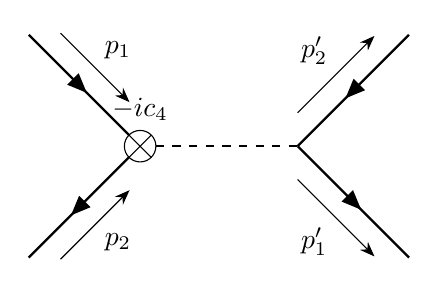
\begin{tikzpicture}[baseline = (a)]
\begin{feynman}[large]
\vertex [crossed dot, label = $-ic_4$] (a) {};
\vertex [below left=of a] (b);
\vertex [above left=of a] (c);
\vertex [right=of a] (d);
\vertex [above right=of d] (o1);
\vertex [below right=of d] (o2);
\diagram* {
(a) -- [fermion, rmomentum=$p_2$] (b),
(c) -- [fermion, momentum=$p_1$] (a),
(a) -- [scalar] (d),
(o1) -- [fermion, rmomentum'=$p_2'$] (d) -- [fermion, momentum'=$p_1'$] (o2)
};
\end{feynman}
\end{tikzpicture}
\end{equation*}
which gives an amplitude,
\[ i\mathcal{M}_a = (-ig) [-ig \tilde{\Gamma}(p_1, p_2)] \cdot \frac{i}{(p_1 + p_2)^2   - m^2} \]

\subsubsection{Class (b)}
Vertical middle loop diagrams look like,
\begin{equation*}
\feynmandiagram [baseline = (l), vertical' = l to b] {
a -- [fermion, rmomentum'=$p_2'$] b -- [fermion, rmomentum'=$p_2$] c,
b -- [scalar] l [blob],
l -- [scalar] d,
f2 -- [fermion, momentum'=$p_1$] d -- [fermion, momentum'=$p_1'$] f1,
};
\quad
=
\quad
\feynmandiagram [baseline = (l2.base), vertical' = d to b] {
a -- [fermion, rmomentum'=$p_2'$] b -- [fermion, rmomentum'=$p_2$] c,
b -- [scalar] l1 
-- [fermion, half left, looseness=1.5] l2 
--[fermion, half left, looseness=1.5] l1,
l2 -- [scalar] d,
f2 -- [fermion, momentum'=$p_1$] d -- [fermion, momentum'=$p_1'$] f1,
};
\quad 
+
\quad
\feynmandiagram [baseline = (l.base), vertical' = d to b] {
a -- [fermion, rmomentum'=$p_2'$] b -- [fermion, rmomentum'=$p_2$] c,
b -- [scalar] l [crossed dot],
l -- [scalar] d,
f2 -- [fermion, momentum'=$p_1$] d -- [fermion, momentum'=$p_1'$] f1,
};
\end{equation*}
which give an amplitude,
\[ i\mathcal{M}_b =  (-ig)^2 \frac{i}{(p_1 - p_1')^2   - m^2} \cdot\left[ -i \Sigma_\phi([p_1 - p_1']^2) \right] \cdot \frac{i}{(p_1 - p_1')^2   - m^2}  \]
\subsubsection{Class (c)}
The next set of diagrams look like,
\begin{equation*}
\begin{tikzpicture}[baseline = (b)]
\begin{feynman}[large]
\vertex (b);
\vertex [above left=of b] (a);
\vertex [below left=of b] (c);
\vertex [right=of b, blob] (d) {};
\vertex [above right=of d] (e);
\vertex [below right=of d] (f);
\diagram* {
(a) -- [fermion, momentum = $p_1$] (b) -- [fermion, rmomentum = $p_2$] (c),
(b) -- [scalar, momentum=$p_1 + p_2$] (d)
(e) -- [fermion, rmomentum' = $p_1'$] (d) -- [fermion, momentum' = $p_2'$] (f)
};
\end{feynman}
\end{tikzpicture}
\quad
\mathlarger{=}
\quad 	
\feynmandiagram [horizontal = b to a, baseline = (a)] {
	a -- [fermion] t1 -- [fermion, momentum=$p_1'$] i1,
	i2 -- [fermion, rmomentum=$p_2'$] t2 -- [fermion] a, 
	t1 -- [scalar] t2,
	a -- [scalar] b,
	o1 -- [fermion, momentum=$p_2$] b -- [fermion, rmomentum=$p_1$] o2
	};
\quad
\mathlarger{+}
\quad 	
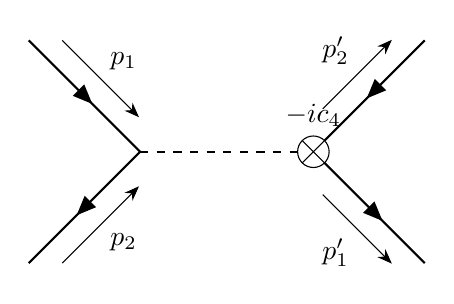
\begin{tikzpicture}[baseline = (a)]
\begin{feynman}[large]
\vertex (a);
\vertex [below left=of a] (b);
\vertex [above left=of a] (c);
\vertex [right=of a, crossed dot, label = $-ic_4$] (d) {};
\vertex [above right=of d] (o1);
\vertex [below right=of d] (o2);
\diagram* {
(a) -- [fermion, rmomentum=$p_2$] (b),
(c) -- [fermion, momentum=$p_1$] (a),
(a) -- [scalar] (d),
(o1) -- [fermion, rmomentum'=$p_2'$] (d) -- [fermion, momentum'=$p_1'$] (o2)
};
\end{feynman}
\end{tikzpicture}
\end{equation*}
which gives an amplitude,
\[ i\mathcal{M}_c = (-ig)[ -ig \tilde{\Gamma}(p_1', p_2')] \cdot \frac{i}{(p_1 + p_2)^2   - m^2} \]


\subsubsection{Class (d)}
These diagrams are similar,
\begin{center}
\feynmandiagram [baseline=(b.base), vertical=a to b] {
i1 -- [fermion, rmomentum=$p_1'$] a [blob],
i2 -- [fermion, momentum'=$p_1$] a,
f1 -- [fermion, rmomentum'=$p_2'$] b -- [fermion, rmomentum'=$p_2$] f2,
a -- [scalar, momentum'=$p_1 - p_1'$] b
};
\end{center}
which give an amplitude,
\[ i\mathcal{M}_d = (-ig) [-ig \tilde{\Gamma}(p_1, -p_1')] \cdot \frac{i}{(p_1 - p_1')^2   - m^2} \]

\subsubsection{Class (e)}
The horizontal middle loop diagrams,
\begin{equation*}
\feynmandiagram [baseline = (l.base), horizontal =b to d] {
a -- [fermion, momentum=$p_1$] b -- [fermion, rmomentum=$p_2$] c,
b -- [scalar] l [blob],
l -- [scalar] d,
f2 -- [fermion, rmomentum=$p_1'$] d -- [fermion, momentum=$p_2'$] f1,
};
\quad
=
\quad
\feynmandiagram [baseline=(b.base), horizontal=b to d] {
a -- [fermion, momentum=$p_1$] b -- [fermion, rmomentum=$p_2$] c,
b -- [scalar] l1 
-- [fermion, half left, looseness=1.5] l2 
--[fermion, half left, looseness=1.5] l1,
l2 -- [scalar] d,
f2 -- [fermion, rmomentum=$p_1'$] d -- [fermion, momentum=$p_2'$] f1,
};
\quad 
+
\quad
\feynmandiagram [baseline = (l.base), horizontal =b to d] {
a -- [fermion, momentum=$p_1$] b -- [fermion, rmomentum=$p_2$] c,
b -- [scalar] l [crossed dot, label = $-ic_3$],
l -- [scalar] d,
f2 -- [fermion, rmomentum=$p_1'$] d -- [fermion, momentum=$p_2'$] f1,
};
\end{equation*}
give an amplitude,
\[ i \mathcal{M}_e = (-ig)^2 \frac{i}{(p_1 + p_2)^2 - m^2} \left[- i \Sigma_\phi([p_1 + p_2]^2) \right] \frac{i}{(p_1 + p_2)^2 - m^2} \]

\subsubsection{Class (f)}
And finally,
\begin{center}
\feynmandiagram [baseline=(b.base), vertical=b to a] {
i1 -- [fermion, momentum=$p_2$] a [blob],
i2 -- [fermion, rmomentum'=$p_2'$] a,
f1 -- [fermion, momentum'=$p_1$] b -- [fermion, momentum'=$p_2'$] f2,
a -- [scalar, rmomentum=$p_1 - p_1'$] b
};
\end{center}
which give an amplitude,
\[ i\mathcal{M}_f = (-ig) [-ig \tilde{\Gamma}(p_2, -p_2')] \cdot \frac{i}{(p_1 - p_1')^2   - m^2} \]

\subsubsection{Box Diagrams}

There are four Box diagrams at the one-loop level,

\begin{equation*}
\feynmandiagram [horizontal=s4 to s1] {
i1 -- [fermion, rmomentum'=$p_2'$] s1 -- [fermion] s2 -- [fermion, momentum'=$p_1'$] i2,
f1 -- [fermion, momentum'=$p_1$] s3 -- [fermion] s4 -- [fermion, rmomentum'=$p_2$] f2,
s1 -- [scalar] s4,
s2 -- [scalar] s3
};
\quad 
\feynmandiagram [horizontal=s1 to s2] {
f1 -- [fermion, momentum'=$p_1$] s1 -- [fermion] s2 -- [fermion, momentum'=$p_1'$] i1,
i2 -- [fermion, momentum=$p_2$] s4 -- [fermion] s3 -- [fermion, momentum=$p_2'$] f2,
s1 -- [scalar] s4,
s2 -- [scalar] s3
};
\quad 
\begin{tikzpicture}
\begin{feynman}
\vertex (i1) ;
\vertex [below right=of i1] (s1);
\vertex [right=of s1] (s2);
\vertex [below=of s2] (s3);
\vertex [left=of s3] (s4);
\vertex [below left=of s4] (i2);
\vertex [below right=of s3] (f2);
\vertex [above right=of s2] (f1);
\diagram* {
(i1) -- [fermion, momentum'=$p_1$] (s1) -- [fermion] (s4) -- [fermion, rmomentum'=$p_2$] (i2),
(f2) -- [fermion, rmomentum'=$p_2'$] (s3) -- [fermion] (s2) -- [fermion, momentum'=$p_1'$] (f1),
(s1) -- [scalar] (s3)
(s2) -- [scalar] (s4)
};
\end{feynman}
\end{tikzpicture}
\quad
\begin{tikzpicture}
\begin{feynman}
\vertex (i1) ;
\vertex [below right=of i1] (s1);
\vertex [right=of s1] (s2);
\vertex [below=of s2] (s3);
\vertex [left=of s3] (s4);
\vertex [below left=of s4] (i2);
\vertex [below right=of s3] (f2);
\vertex [above right=of s2] (f1);
\diagram* {
(i1) -- [fermion, momentum'=$p_1$] (s1) -- [fermion] (s2) -- [fermion, momentum'=$p_1'$] (f1),
(f2) -- [fermion, rmomentum'=$p_2'$] (s3) -- [fermion] (s4) -- [fermion, rmomentum'=$p_2$] (i2),
(s1) -- [scalar] (s3)
(s2) -- [scalar] (s4)
};
\end{feynman}
\end{tikzpicture}
\end{equation*}

The amplitudes for each of these terms can be transformed into one another by swapping the values of the incoming/outgoing momenta and shifting the value of the undetermined momentum. It can be shown either by writing down the integrals explicitly or diagram chasing that the amplitude for these diagrams are,
\[ i \mathcal{M}_{box} = i \mathcal{M}_B(p_1, p_2, p_1', p_2') + i \mathcal{M}_B(p_1, -p_1', -p_2, p_2') + i \mathcal{M}_B(p_1, p_2, p_2', p_1') + i \mathcal{M}_B(p_1, -p_1', p_2', -p_2)\]
where each term corresponds to the respective box diagram shown above.  

\subsubsection{Tree-Level Diagrams}

As before, we have the two tree-level diagrams,
\begin{figure}
\centering
\begin{minipage}{.5\textwidth}
  \centering
  
\feynmandiagram [vertical'=a to b] {
i1 -- [fermion, momentum' = \(p_1\)] a -- [fermion, momentum' = \(p_1'\)] f1,
a -- [scalar] b,
f2 -- [anti fermion, momentum = \(p_2\)] b -- [anti fermion, momentum = \(p_2'\)] i2,
};


\end{minipage}%
\begin{minipage}{.5\textwidth}
  \centering
  
\feynmandiagram [horizontal=a to b] {
i1 -- [fermion, momentum = \(p_1\)] a -- [fermion, rmomentum = \(p_2\)] i2,
a -- [scalar] b,
f1 -- [fermion, rmomentum' = \(p_1'\)] b -- [fermion, momentum' = \(p_2'\)] f2,
};

\end{minipage}
\end{figure}
with total amplitude,
\[ i \mathcal{M}_{tree} = (-ig)^2 \left[\frac{i}{(p_1 - p_1')^2 - m^2 } + \frac{i}{(p_1 + p_2)^2 - m^2 }\right] \]

\subsection{The Scattering Cross Section and Field Strength Renormalization}

Finally, the glorious total scattering amplitude is given by the sum of all these contributions. In the center of mass reference frame, remembering the factor of $Z_\psi^{1/2}$ which appear due to the LSZ reduction formula expression for the $S$ matrix, the differential scattering cross section is given by,
\begin{align*}
\deriv{\sigma}{\Omega} & = \frac{|Z^2_{\psi} \mathcal{M}|^2}{64 \pi^2 E_{CM}^2}
\\
& = \frac{Z^4_{\psi}}{64 \pi^2 E_{CM}^2} \left| \mathcal{M}_a + \mathcal{M}_b + \mathcal{M}_c + \mathcal{M}_d + \mathcal{M}_e + \mathcal{M}_f + \mathcal{M}_{box} + \mathcal{M}_{tree} \right|^2 
\end{align*}
Because of our incomplete renormalization prescription, this scattering cross section is carrying around awkward factors of $Z_\psi^{1/2}$. Since the entire expression is proportional to $g^4$ we might consider rescaling the coupling constant $g$ to $g' = Z_\psi^{1/2} g$ such that there is no explicit dependence on $Z_\psi$ out front. This is not quite right, as we will more explicitly see, because it does not account for the terms in $\mathcal{M}$ which depend on higher powers of $g$. We also see hints that our coupling constant might be wrong by seriously considering our vertex renormalization condition. We imposed that $-i \Gamma(p_1, p_2) = -ig$, the physical coupling constant, at a specific renormalization point. However, if one calculates out diagrams contributing to the vertex function, the LSZ reduction formula\footnote{While these diagrams cannot conserve momentum on shell and thus cannot be interpreted as scattering amplitudes, the pole structure of their associated correlation functions should align with the LSZ calculation and would produce the same overall factor (when the dressed propagators attached to the vertex diagrams are included) when included as a sub-diagram of a larger physically possible scattering process.} implies that the amplitude should contain a factor of $Z_\psi^2 Z_\phi^{1/2}$. So we are actually renormalizing our physical coupling constant at $- i Z_\psi Z_\phi^{1/2} g$ meaning that $g$ is not the truly physical coupling parameter of the theory. \bigskip\\
To fix this issue once and for all, let us return to the unrenormalized Lagrangian,
\[ \lagrange = \lagrange_0 + \lagrange_{\ipic} \quad \quad \lagrange_0 = \tfrac{1}{2} \partial_\mu \phi_0 \partial^\mu \phi_0 - \tfrac{1}{2} m_0^2 \phi^2 + \partial_\mu \dpsi_0 \partial^\mu \psi_0 - M_0^2 \dpsi_0 \psi_0 \quad \quad \lagrange_{\ipic} = -g_0 \dpsi \psi \meson \]  
where zeros indicate the bare parameters. The first step is to shift the the constants to more physical values (which I will label with a one) by putting the difference into counterterms,
\[ \lagrange = \tfrac{1}{2} \partial_\mu \phi_0 \partial^\mu \phi_0 - \tfrac{1}{2} m_1^2 \phi^2 + \partial_\mu \dpsi_0 \partial^\mu \psi_0 - M_1^2 \dpsi \psi - g_1 \dpsi_0 \psi_0 \meson_0 - c_0 - c_1 \phi_0 - c_2 \dpsi_0 \psi_0 -\tfrac{1}{2} c_3 \phi_0^2 - c_4 \dpsi_0 \psi_0 \phi_0 \]  
However, we have yet to fix the issue of residues in the dressed propagator. To do this, re-scale the fields, $\phi_0 = Z^{1/2}_\phi \phi$ and $\psi = Z^{1/2}_\psi \psi$ which contributes a factor of $Z^{-1/2}$ for each field in a correlation function and thus fixes the pole structure of the exact dressed propagator that would appear in the LSZ reduction formula as,
\[ \tilde{G}^{(2)}(p) = \frac{i}{p^2 - m^2 + i \epsilon} \] 
for a stable particle and for an unstable particle, the two point function becomes,
\[ \tilde{G}^{(2)}(p) = \frac{i}{p^2 - m^2 + i m \Gamma} \] 
The Lagrangian becomes,
\begin{align*}
\lagrange & = \tfrac{1}{2} Z_\phi \partial_\mu \phi \partial^\mu \phi - Z_\phi \tfrac{1}{2} m_1^2 \phi^2 + Z_\psi \partial_\mu \dpsi \partial^\mu \psi - Z_\psi M_1^2 \dpsi \psi - Z_\psi Z_\phi^{1/2} g_1 \dpsi \psi \meson 
\\
& - c_0 - c_1 Z_\phi^{1/2} \phi - c_2 Z_\psi \dpsi \psi - Z_\phi \tfrac{1}{2} c_3 \phi^2 - Z_\psi Z_\phi^{1/2} c_4 \dpsi \psi \phi
\end{align*} 
which explains why $Z_\psi Z_\phi^{1/2} g_1$ seemed to be the more physical quantity in the partially renormalized theory. However, if we are going to expand this Lagrangian in perturbation theory, we want our non-interacting part to look like the free theories we have previously considered. To do this, we can offload the difference into counterterms, 
\[ \lagrange = \tfrac{1}{2} \partial_\mu \phi \partial^\mu \phi -  \tfrac{1}{2} m^2 \phi^2 + \partial_\mu \dpsi \partial^\mu \psi - M_1^2 \dpsi \psi - g \dpsi \psi \meson - c_0 - c_1 \phi - c_2 \dpsi \psi - \tfrac{1}{2} c_3 \phi^2 - c_4 \dpsi \psi \phi - c_5 \tfrac{1}{2} \partial_\mu \phi \partial^\mu \phi - c_6 \partial_\mu \dpsi \partial^\mu \psi \] 
where $c_2 = M_0^2 Z_\psi - M^2$ and $c_3 = \tfrac{1}{2} (m_0^2 Z_\phi - m^2)$ and $c_5 = Z_\phi - 1$ and $c_6 = Z_\psi - 1$. 
Now the free Lagrangian is written solely in terms of physical measurable quantities. 
Putting the counterterms into the interacting part of the Lagrangian, the Feynman rules (specifically vertex rules) are only slightly altered, 
	\begin{equation*}
	\feynmandiagram[horizontal = b to a, small, inline = (a)] {
	i1 -- [fermion] a -- [fermion] f1,
	a -- [scalar] b
	}; = - i g
	\hspace{2cm}
	\feynmandiagram[horizontal = i1 to o1, small, inline = (c),  tree layout] {
	i1 -- [fermion] c [crossed dot] -- [fermion] o1
	}; = - i (c_2 - p^2 c_6)
	\hspace{2cm}
	\feynmandiagram[horizontal = i1 to o1, small, inline = (c),  tree layout] {
	i1 -- [scalar] c [crossed dot] -- [scalar] o1
	}; = - i (c_3 - p^2 c_5)
	\end{equation*}
The only place in our derivations where this matters is in the calculation of the one-particle irreducible terms $-i \Sigma(p^2)$. We now have stricter renormalization conditions, $\mathrm{Re}[\Sigma(p^2 = m^2)] = 0$ and $\deriv{\Sigma}{p^2} \bigg|_{p^2 = m^2} = 0$ to retain the form of the dressed propagator. This extra condition fixes the counterterms $c_5$ and $c_6$. Matching the counterterms, the new field strength normalized one-particle irreducible amplitude is,
\[ - i \Sigma(p^2) = - i \Sigma^{(old)}(p^2) + i (p^2 - m^2) \deriv{\Sigma^{(old)}}{p^2} \] 
By some amazing feat of clairvoyance, we have already computed this amplitude. 
Beyond that, calculations in this renormalization prescription are identical except for the fact that vertex renormalization now has a more physical meaning. To get single vertex amplitudes to work out correctly in the non-renormalized theory, we can fix $g_1$ by the condition $g = Z_\psi Z_\phi^{1/2} g_1$ where $g$ is taken to be the physical coupling constant and zero momentum. Now, we will consider the physically measurable differential cross section as calculated in these two different renormalization prescriptions. In terms of the old non-renormalized (not field strength renormalized) variables,
\begin{align*}
\deriv{\sigma^{(old)}}{\Omega} & = \frac{|Z^2_{\psi} \mathcal{M}|^2}{64 \pi^2 E_{CM}^2}
\\
& = \frac{Z^4_{\psi}}{64 \pi^2 E_{CM}^2} \left| \mathcal{M}_a + \mathcal{M}_b + \mathcal{M}_c + \mathcal{M}_d + \mathcal{M}_e + \mathcal{M}_f + \mathcal{M}_{box} + \mathcal{M}_{tree} \right|^2 
\\
& = \frac{g_1^4 Z^4_{\psi}}{64 \pi^2 E_{CM}^2} \left|  \frac{i\tilde{\Gamma}(p_1, p_2)}{s  - m^2} + \frac{i}{t - m^2} \cdot\left[ -i \Sigma_\phi^{(old)}(t) \right] \cdot \frac{i}{t - m^2} + \frac{i \tilde{\Gamma}(p_1', p_2')}{s - m^2} 
+  \frac{i\tilde{\Gamma}(p_1, -p_1')}{t - m^2} \right.
\\ 
& \left.
\quad \quad \quad \quad \quad \quad 
+ \frac{i}{s - m^2} \left[- i \Sigma_\phi^{(old)}(s) \right] \frac{i}{s - m^2} + \frac{i \tilde{\Gamma}(p_2, -p_2')}{t - m^2} + i\mathcal{M}_{box}/(-ig)^2 +  \left[\frac{i}{t - m^2 } + \frac{i}{s - m^2 }\right] \right|^2 
\\
& = \frac{g_1^4 Z^4_{\psi}}{64 \pi^2 E_{CM}^2} \left|  \frac{ i\tilde{\Gamma}(p_1, p_2)}{s  - m^2} + \frac{i \Sigma_\phi^{(old)}(t)}{(t - m^2)^2} + \frac{i\tilde{\Gamma}(p_1', p_2')}{s - m^2} 
+  \frac{i\tilde{\Gamma}(p_1, -p_1')}{t - m^2} \right.
\\ 
& \left.
\quad \quad \quad \quad \quad \quad 
+ \frac{i \Sigma_\phi^{(old)}(s)}{(s - m^2)^2} + \frac{i\tilde{\Gamma}(p_2, -p_2')}{t - m^2} + i\mathcal{M}_{box}/(-ig)^2 + \left[\frac{i}{t - m^2 } + \frac{i}{s - m^2 }\right] \right|^2 
\end{align*} 
Since $Z = 1 + O(g^2)$ to the level of perturbation theory we are working, $\Sigma$, $\tilde{\Gamma}$, and $i\mathcal{M}_{box}/(-ig)^2$ which are all quantities of order $g_1^2$ are unchanged by the substitution $g_1 \to g$. The shift in the scattering amplitude due to changing these terms is order $g^6$ (since the entire amplitude is multiplied by a factor of $g^2$) which is above the order of our perturbation theory calculations. Therefore, substituting $g = Z_\psi Z_\phi^{1/2} g_1$ we get,
\begin{align*}
\deriv{\sigma^{(old)}}{\Omega} &= \frac{g^4 Z_\phi^{-2}}{64 \pi^2 E_{CM}^2} \left|  \frac{i \tilde{\Gamma}(p_1, p_2)}{s  - m^2} + \frac{i \Sigma_\phi^{(old)}(t)}{(t - m^2)^2} + \frac{i\tilde{\Gamma}(p_1', p_2')}{s - m^2} 
+  \frac{i\tilde{\Gamma}(p_1, -p_1')}{t - m^2} \right.
\\ 
& \left.
\quad \quad \quad \quad \quad \quad 
+ \frac{i \Sigma_\phi^{(old)}(s)}{(s - m^2)^2} + \frac{i\tilde{\Gamma}(p_2, -p_2')}{t - m^2} + i\mathcal{M}_{box}/(-ig)^2 + \left[\frac{i}{t - m^2 } + \frac{i}{s - m^2 }\right] \right|^2 
\end{align*}  
Now, I will apply the factor of $Z_\phi^{-2}$ to each term. However, since we are only working to order $g^4$, any term of order above $g$ will be unchanged by the multiplication of $Z_\phi = 1 + O(g^2)$. Therefore, only the tree-level terms are affected,
\begin{align*}
\deriv{\sigma^{(old)}}{\Omega} &= \frac{g^4 Z_\phi^{-2}}{64 \pi^2 E_{CM}^2} \left|  \frac{ i\tilde{\Gamma}(p_1, p_2)}{s  - m^2} + \frac{i \Sigma_\phi^{(old)}(t)}{(t - m^2)^2} + \frac{i\tilde{\Gamma}(p_1', p_2')}{s - m^2} 
+  \frac{i\tilde{\Gamma}(p_1, -p_1')}{t - m^2} \right.
\\ 
& \left.
\quad \quad \quad \quad \quad \quad 
+ \frac{i \Sigma_\phi^{(old)}(s)}{(s - m^2)^2} + \frac{i\tilde{\Gamma}(p_2, -p_2')}{t - m^2} + i\mathcal{M}_{box}/(-ig)^2 + Z_\phi^{-1} \left[\frac{i}{t - m^2 } + \frac{i}{s - m^2 }\right] \right|^2 
\end{align*}  
Using the formula for $Z_\phi^{-1} = 1 - \deriv{\Sigma_\phi^{(old)}}{p^2} \bigg|_{p^2 = m^2}$ we get,
\begin{align*}
\deriv{\sigma^{(old)}}{\Omega} &= \frac{g^4}{64 \pi^2 E_{CM}^2} \left|  \frac{i\tilde{\Gamma}(p_1, p_2)}{s  - m^2} + \frac{i \Sigma_\phi^{(old)}}{(t - m^2)^2} + \frac{i\tilde{\Gamma}(p_1', p_2')}{s - m^2} 
+  \frac{i\tilde{\Gamma}(p_1, -p_1')}{t - m^2} \right.
\\ 
& \left.
\quad \quad \quad \quad \quad \quad 
+ \frac{i \Sigma_\phi^{(old)}(s)}{(s - m^2)^2} + \frac{i\tilde{\Gamma}(p_2, -p_2')}{t - m^2} + i\mathcal{M}_{box}/(-ig)^2 + \left( 1 - \deriv{\Sigma_\phi^{(old)}}{p^2} \right) \left[\frac{i}{t - m^2 } + \frac{i}{s - m^2 }\right] \right|^2  
\\
&= \frac{g^4}{64 \pi^2 E_{CM}^2} \left|  \frac{ i\tilde{\Gamma}(p_1, p_2)}{s  - m^2} + \frac{i \Sigma_\phi^{(old)}(t) - i(t - m^2) \deriv{\Sigma_\phi^{(old)}}{p^2}}{(t - m^2)^2} + \frac{i\tilde{\Gamma}(p_1', p_2')}{s - m^2} 
+  \frac{i\tilde{\Gamma}(p_1, -p_1')}{t - m^2} \right.
\\ 
& \left.
\quad \quad \quad \quad \quad \quad 
+ \frac{i \Sigma_\phi^{(old)}(s) - i(s - m^2) \deriv{\Sigma_\phi^{(old)}}{p^2} }{(s - m^2)^2} + \frac{i\tilde{\Gamma}(p_2, -p_2')}{t - m^2} + i\mathcal{M}_{box}/(-ig)^2 + \left[\frac{i}{t - m^2 } + \frac{i}{s - m^2 }\right] \right|^2
\\
&= \frac{g^4}{64 \pi^2 E_{CM}^2} \left|  \frac{i \tilde{\Gamma}(p_1, p_2)}{s  - m^2} + \frac{i \Sigma_\phi(t)}{(t - m^2)^2} + \frac{i\tilde{\Gamma}(p_1', p_2')}{s - m^2} 
+  \frac{i\tilde{\Gamma}(p_1, -p_1')}{t - m^2} \right.
\\ 
& \left.
\quad \quad \quad \quad \quad \quad 
+ \frac{i \Sigma_\phi(s)}{(s - m^2)^2} + \frac{i\tilde{\Gamma}(p_2, -p_2')}{t - m^2} + i\mathcal{M}_{box}/(-ig)^2 + \left[\frac{i}{t - m^2 } + \frac{i}{s - m^2 }\right] \right|^2    
\end{align*}  
which is the scattering cross section in the form given by the fully renormalized theory. The fact that both theories predict the same physically measurable scattering cross section is comforting and checks that we performed our field strength renormalization prescription correctly. Now it is finally time to explicitly compute this cross section.

\subsection{Center of Mass Frame Calculations}

Although we have computed a valid expression for the scattering cross section, it is not much use without further simplifications. First, notice that the reduced vertex function only appears with on-shell momentum arguments. Therefore, we can simplify,
\[\tilde{\Gamma}_{on-shell}(p_1, p_2) = \frac{ g^2}{16 \pi^2} \left[ \int_0^1 \frac{\d{x} \d{y} \d{z} \delta(x + y + z - 1)}{(y p_1 - z p_2)^2 + x m^2 - i \epsilon} - \int_0^1 \frac{\d{x} \d{y} \d{z} \delta(x + y + z - 1)}{(y - z)^2 M^2 + x m^2} \right]\]
The next simplification comes from the facts of two particle scattering in the center of mass frame. In this reference frame, we can write our four momentum fourvectors as,
\[ p_1 = (E, \vec{p}) \quad p_2 = (E, -\vec{p}) \quad p_1' = (E, \vec{p'}) \quad p_2' = (E, -\vec{p'}) \]
With this parametrization, the Mandelstam parameters become,
\[ s = (p_1 + p_2)^2 = 4 E^2 \quad t = (p_1 - p_1')^2 = -2 \vec{p}^{\, 2} (1 - \cos{\Theta}) \quad u = (p_1 - p_2')^2 = -2 \vec{p}^{\, 2} (1 + \cos{\Theta}) \]
Now we need to simplify the eight integrals,
\begin{align*} 
\tilde{\Gamma}_{on-shell}(p_1, p_2) &= \frac{g^2}{16 \pi^2} \int_0^1 \frac{\d{x} \d{y} \d{z} \delta(x + y + z - 1)}{(y - z)^2 E^2 - (y + z)^2 \vec{p}^{\, 2} + x m^2 - i \epsilon} + c_4
\\
& = \frac{g^2}{16 \pi^2} \int_0^1 \frac{\d{x} \d{y} \d{z} \delta(x + y + z - 1) }{(y - z)^2 (M^2 + \vec{p}^{\, 2}) - (y + z)^2 \vec{p}^{\, 2} + x m^2 - i \epsilon} + c_4
\\
& = \frac{g^2}{16 \pi^2} \int_0^1 \frac{ \d{x} \d{y} \d{z} \delta(x + y + z - 1) }{(y + z)^2 M^2 - yz s + x m^2 - i \epsilon} + c_4
\end{align*}
Denote this function as $\tilde{\Gamma}(s)$.
Similarly, $\tilde{\Gamma}(p_1', p_2') = \tilde{\Gamma}(s)$ since the integral is expressed only in terms of rotationally invariant quantities and $(p_1', p_2')$ is a rotation of $(p_1, p_2)$ through the scattering angle.
Next, we need to calculate, 
\begin{align*} 
\tilde{\Gamma}_{on-shell}(p_1, -p_1') &= \frac{g^2}{16 \pi^2} \int_0^1 \frac{\d{x} \d{y} \d{z} \delta(x + y + z - 1)}{(y + z)^2 (M^2 + \vec{p}^{\, 2}) - (y^2 + z^2 + 2 yz \cos{\Theta}) \vec{p}^{\, 2}+ x m^2 - i \epsilon} + c_4 
\\
& = \frac{g^2}{16 \pi^2} \int_0^1 \frac{\d{x} \d{y} \d{z} \delta(x + y + z - 1)}{(y + z)^2 M^2 + 2yz(1 - \cos{\Theta})\vec{p}^{\, 2} + x m^2 - i \epsilon}
\\
& = \frac{g^2}{16 \pi^2} \int_0^1 \frac{\d{x} \d{y} \d{z} \delta(x + y + z - 1) }{(y + z)^2M^2 - yz t + x m^2 - i \epsilon} + c_4
\end{align*}
This is the same function $\tilde{\Gamma}(t)$ simply with $s$ replaced with $u$. Similarly, $\tilde{\Gamma}(p_2, p_2') = \tilde{\Gamma}(t)$ because this integral is invariant under parity inversion and $(p_2, p_2')$ is a inversion through the center of mass of $(p_1, p_1')$.
All the vertex functions can be expressed in terms of a single function $\tilde{\Gamma}(\alpha)$ which is plotted below. This function represents the dependence of the effective coupling constant on the scattering energy.

\begin{figure}[!htb]
    \centering
    \begin{minipage}[b]{.45\textwidth}
        \centering
        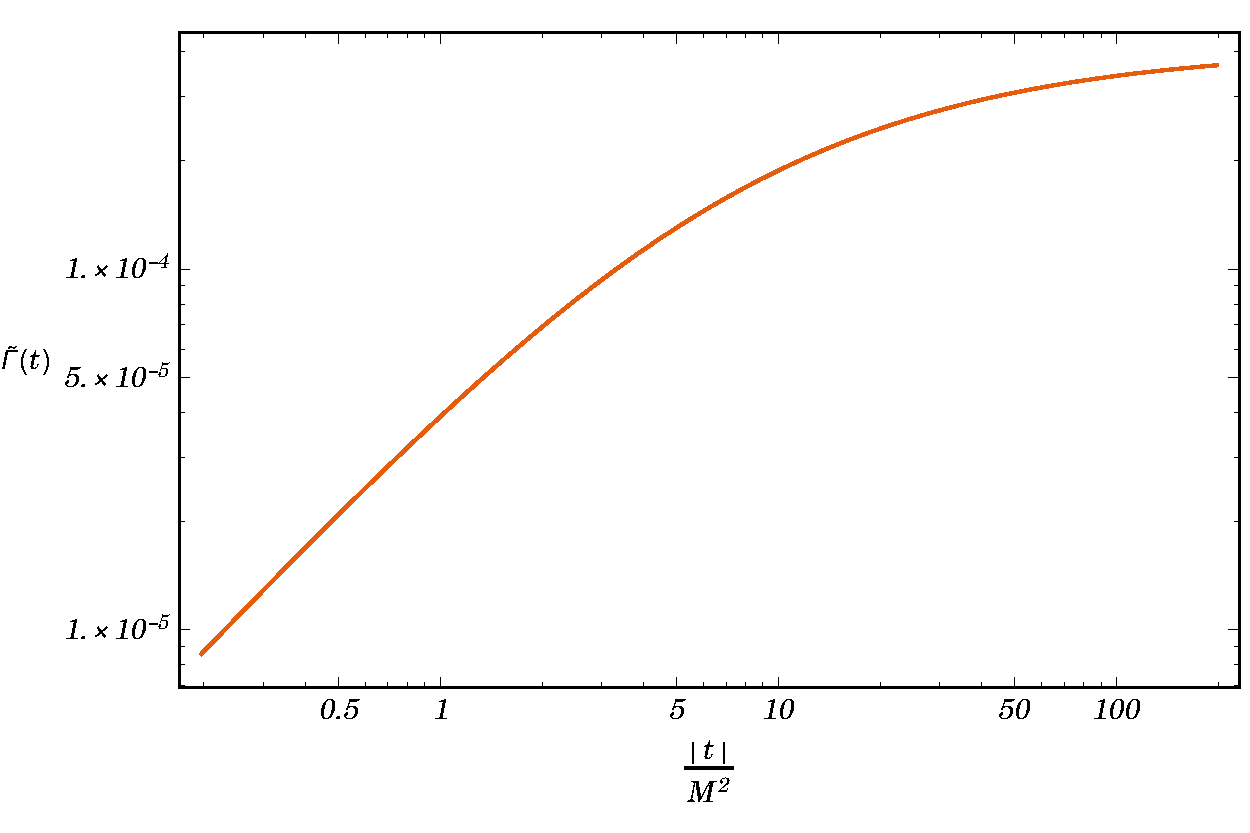
\includegraphics[width=9cm, height=7cm]	{Gamma-t-channel}
        \caption{The absolute value of the reduced vertex Function $\tilde{\Gamma}(t)$ for the $t$-channel process using parameters $m = 0.5M$ and $g = 0.25M$.}
        \label{fig:gamma1}
    \end{minipage}%
    \hfill
    \begin{minipage}[b]{0.45\textwidth}
        \centering
        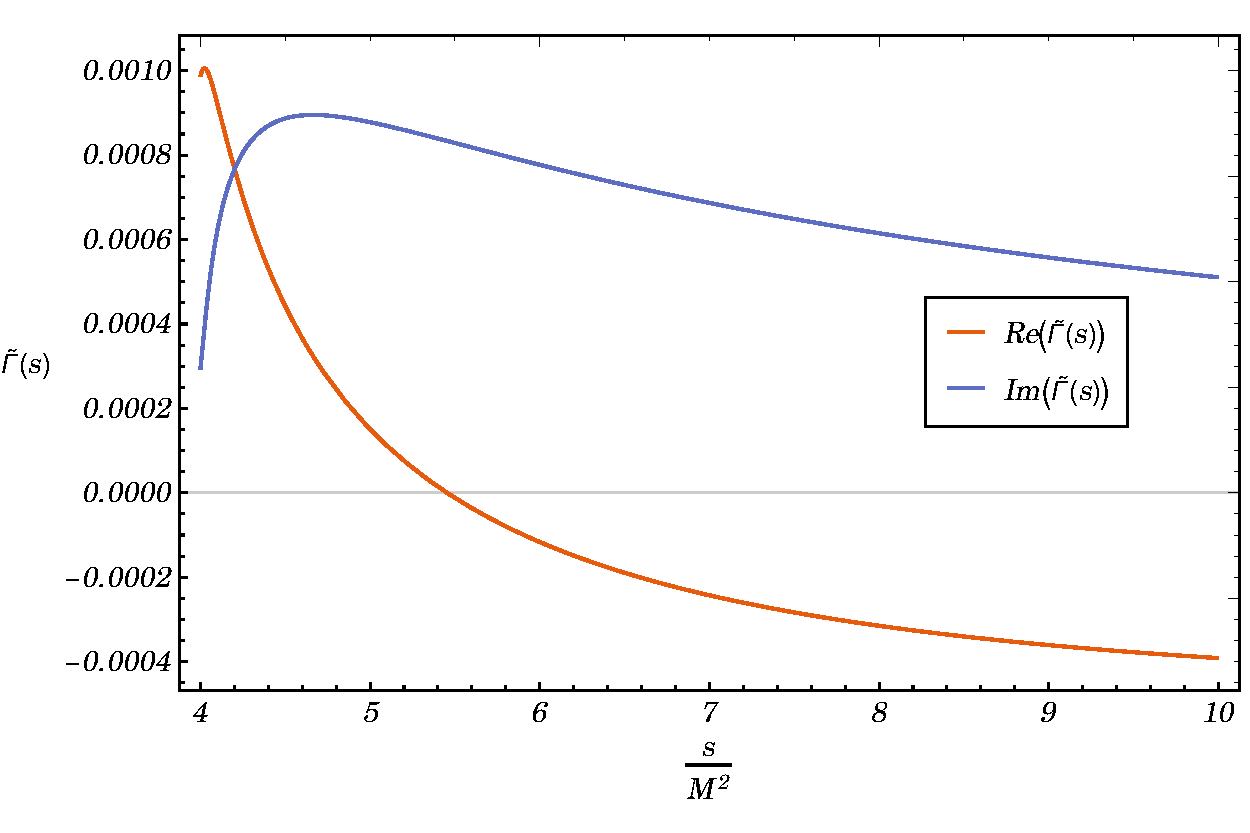
\includegraphics[width=9cm, height=7cm]{Gamma-s-channel}
        \caption{The reduced vertex Function $\tilde{\Gamma}(t)$ for the $s$-channel process in the stable meson regime using parameters $m = 0.5M$ and $g = 0.25M$.}
        \label{fig:gamma1}
    \end{minipage}
\end{figure}

Now we need to calculate the box diagram integrals,
\begin{align*}  
i\mathcal{M}_B(p_1, p_2, p_1', p_2') &= \frac{ig^4}{16 \pi^2} \int_{0}^{1} \frac{\d{x} \d{y} \d{z} \d{w} \delta(x + y + z + w - 1) }{[(y p_1 + z (p_1 + p_2) + w p_1' )^2 - z (p_1 + p_2)^2 + (x + z)m^2 - i \epsilon]^2} 
\\
& = \frac{ig^4}{16 \pi^2} \int_{0}^{1} \frac{\d{x} \d{y} \d{z} \d{w} \delta(x + y + z + w - 1) }{[(y + 2 z + w)^2 (M^2 + \vec{p}^{\, 2}) - \vec{p}^{\, 2}(y^2 + w^2 + 2 yw \cos{\Theta}) - z s + (x + z)m^2 - i \epsilon]^2} 
\\
& = \frac{ig^4}{16 \pi^2} \int_{0}^{1} \frac{\d{x} \d{y} \d{z} \d{w} \delta(x + y + z + w - 1) }{[M^2 (y + w)^2 - yw t + (y + w)z s + (z^2 - z)s + (x + z)m^2 - i \epsilon]^2} 
\end{align*}
similarly,
\begin{align*}  
i\mathcal{M}_B(p_1, -p_1', -p_2, p_2') & = \frac{ig^4}{16 \pi^2} \int_{0}^{1} \frac{\d{x} \d{y} \d{z} \d{w} \delta(x + y + z + w - 1) }{[M^2 (y + w)^2 - yw s + (y + w)z t + (z^2 - z) t + (x + z)m^2 - i \epsilon]^2} 
\\
i\mathcal{M}_B(p_1, p_2, p_2', p_1') & = \frac{ig^4}{16 \pi^2} \int_{0}^{1} \frac{\d{x} \d{y} \d{z} \d{w} \delta(x + y + z + w - 1) }{[M^2 (y + w)^2 - yw u + (y + w)z s + (z^2 - z) s + (x + z)m^2 - i \epsilon]^2} 
\\
i\mathcal{M}_B(p_1, -p_1', p_2', -p_2) & = \frac{ig^4}{16 \pi^2} \int_{0}^{1} \frac{\d{x} \d{y} \d{z} \d{w} \delta(x + y + z + w - 1) }{[M^2 (y + w)^2 - yw u + (y + w)z t + (z^2 - z) t + (x + z)m^2 - i \epsilon]^2} 
\end{align*}
Therefore, these three integrals are all expressible in terms of a single function,
\[ B(a,b) = -\frac{g^2}{16 \pi^2} \int_{0}^{1} \frac{\d{x} \d{y} \d{z} \d{w} \delta(x + y + z + w - 1) }{[M^2 (y + w)^2 - yw a + (y + w)z b + (z^2 - z) b + (x + z)m^2 - i \epsilon]^2} \]
In terms of this function,
\begin{align*}
(-ig)^2 B(t, s) &= \mathcal{M}_B(p_1, p_2, p_1', p_2') \\
(-ig)^2 B(s, t) &= \mathcal{M}_B(p_1, -p_1', -p_2, p_2') \\
(-ig)^2 B(u, s) &= \mathcal{M}_B(p_1, p_2, p_2', p_1') \\
(-ig)^2 B(u, t) &= \mathcal{M}_B(p_1, -p_1', p_2', -p_2) 
\end{align*}
Therefore,
\[\mathcal{M}_{box} = (-ig)^2[B(t, s) + B(s, t) + B(u, s) + B(u,t)]\]
The $B$ integral must be computed numerically.
Now we have all the tools to evaluate the explicit scattering cross section in the center of mass reference frame. In terms of these new functions,
\begin{align*}
\deriv{\sigma}{\Omega} 
&= \frac{g^4}{64 \pi^2 s} \left| \frac{i}{t - m^2} + \frac{i}{s - m^2} + \frac{2i \tilde{\Gamma}(s)}{s - m^2} + \frac{2i \tilde{\Gamma}(t)}{t - m^2} + \frac{i \Sigma_\phi(t)}{(t - m^2)^2} + \frac{i \Sigma_\phi(s)}{(s - m^2)^2} + i B(t, s) + i B(s, t) + i B(u, s) + i B(u,t)  \right|^2 
\end{align*}

\subsection{Taming Resonance Poles in the Scattering Cross Section}

In the case $m > 2M$ then $s = m^2 > 4 M^2$ is a valid scattering energy and thus there is an unphysical pole in the scattering cross section due to the propagator $\frac{i}{s - m^2}$. However, this pole exists exactly when $\phi$ becomes unstable. This is because if $\phi$ mesons can be produced in scattering experiments then, by time reversal symmetry, $\phi$ must be able to decay. The theory is saved by the fact that an unstable meson shifts the poles of the exact propagator off the real axis. This pole persists to every order in perturbation theory but is absent from the exact theory. To correct this failing of the perturbative approach, we can replace the terms,
\[ \frac{i}{s - m^2} + \frac{i \Sigma_\phi(s)}{(s - m^2)^2} \quad \text{and} \quad \frac{i}{t - m^2} + \frac{i \Sigma_\phi(t)}{(t - m^2)^2} \]
with the exact two-point function i.e. dressed $\phi$ propagators,
\[ \frac{i}{s - m^2 - \Sigma_\phi(s)} \quad \text{and} \quad \frac{i}{t - m^2 - \Sigma_\phi(t)}\]
The terms we have calculated at the one-loop level correspond to the first nontrivial term in the geometric sequence for the exact propagator.
Diagrammatically, this is equivalent to including the following terms above the one-loop level,
\begin{equation*}
\begin{tikzpicture}[baseline = -0.11cm]
\begin{feynman}
\vertex (a);
\vertex [above left=of a, momentum = $p_1$] (i1) ;
\vertex [below left=of a, rmomentum = $p_2$] (i2) 
;
\vertex [right=of a, blob] (b) {\(\mathbf{1PI}\)};
\vertex [right=of b] (c);
\vertex [above right=of c] (f1) ;
\vertex [below right=of c] (f2) ;
\diagram* {
(i1) --[fermion, momentum = $p_1$] (a) -- [fermion, rmomentum = $p_2$] (i2),
(a) -- [scalar] (b) -- [scalar] (c)
(f2) --[fermion, rmomentum = $p_1'$] (c) -- [fermion, momentum = $p_2'$] (f1)
};
\end{feynman}
\end{tikzpicture}
\quad 
+
\quad 
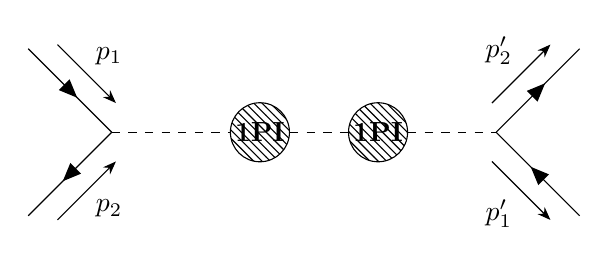
\begin{tikzpicture}[baseline = -0.11cm]
\begin{feynman}
\vertex (a);
\vertex [above left=of a, momentum = $p_1$] (i1) ;
\vertex [below left=of a, rmomentum = $p_2$] (i2) ;
\vertex [right=of a, blob] (b) {\(\mathbf{1PI}\)};
\vertex [right=of b, blob] (c) {\(\mathbf{1PI}\)};
\vertex [right=of c] (d);
\vertex [above right=of d] (f1) ;
\vertex [below right=of d] (f2) ;
\diagram* {
(i1) --[fermion, momentum = $p_1$] (a) -- [fermion, rmomentum = $p_2$] (i2),
(a) -- [scalar] (b) -- [scalar] (c) -- [scalar] (d),
(f2) --[fermion, rmomentum = $p_1'$] (d) -- [fermion, momentum = $p_2'$] (f1)
};
\end{feynman}
\end{tikzpicture}
\end{equation*}
\begin{equation*}
\quad 
+
\quad 
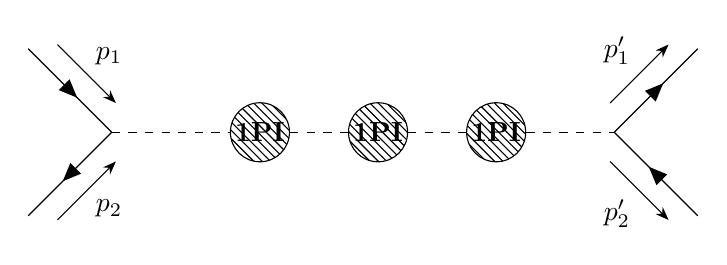
\begin{tikzpicture}[baseline = -0.11cm]
\begin{feynman}
\vertex (a);
\vertex [above left=of a] (i1) ;
\vertex [below left=of a] (i2) ;
\vertex [right=of a, blob] (b) {\(\mathbf{1PI}\)};
\vertex [right=of b, blob] (c) {\(\mathbf{1PI}\)};
\vertex [right=of c, blob] (d) {\(\mathbf{1PI}\)};
\vertex [right=of d] (e);
\vertex [above right=of e] (f1) ;
\vertex [below right=of e] (f2) ;
\diagram* {
(i1) --[fermion, momentum = $p_1$] (a) -- [fermion, rmomentum = $p_2$] (i2),
(a) -- [scalar] (b) -- [scalar] (c) -- [scalar] (d) -- [scalar] (e),
(f2) --[fermion, rmomentum = $p_2'$] (e) -- [fermion, momentum = $p_1'$] (f1)
};
\end{feynman}
\end{tikzpicture}
\quad
+ 
\quad
\cdots
\end{equation*}
and similarly,
\begin{equation*}
\begin{tikzpicture}[baseline = -1.7cm]
\begin{feynman}
\vertex (a);
\vertex [above left=of a, momentum' = $p_1$] (i1) ;
\vertex [above right=of a, rmomentum = $p_2$] (i2) 
;
\vertex [below=of a, blob] (b) {\(\mathbf{1PI}\)};
\vertex [below=of b] (c);
\vertex [below left=of c] (f1) ;
\vertex [below right=of c] (f2) ;
\diagram* {
(i1) --[fermion, momentum' = $p_1$] (a) -- [fermion, momentum' = $p_1'$] (i2),
(a) -- [scalar] (b) -- [scalar] (c)
(f2) --[fermion, rmomentum' = $p_2'$] (c) -- [fermion, rmomentum' = $p_2$] (f1)
};
\end{feynman}
\end{tikzpicture}
\quad 
+
\quad 
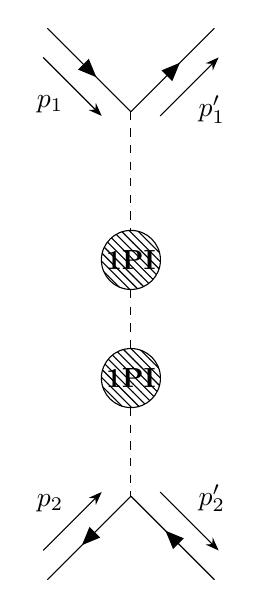
\begin{tikzpicture}[baseline = -2.5cm]
\begin{feynman}
\vertex (a);
\vertex [above left=of a, momentum' = $p_1$] (i1) ;
\vertex [above right=of a, rmomentum = $p_2$] (i2) 
;
\vertex [below=of a, blob] (b) {\(\mathbf{1PI}\)};
\vertex [below=of b, blob] (c) {\(\mathbf{1PI}\)};
\vertex [below=of c] (d);
\vertex [below left=of d] (f1) ;
\vertex [below right=of d] (f2) ;
\diagram* {
(i1) --[fermion, momentum' = $p_1$] (a) -- [fermion, momentum' = $p_1'$] (i2),
(a) -- [scalar] (b) -- [scalar] (c) -- [scalar] (d),
(f2) --[fermion, rmomentum' = $p_2'$] (d) -- [fermion, rmomentum' = $p_2$] (f1)
};
\end{feynman}
\end{tikzpicture}
\quad 
+
\quad 
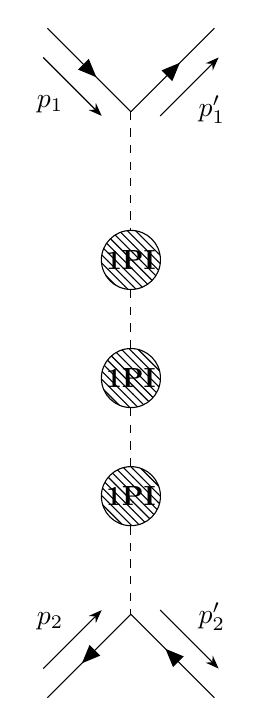
\begin{tikzpicture}[baseline = -3.2cm]
\begin{feynman}
\vertex (a);
\vertex [above left=of a, momentum' = $p_1$] (i1) ;
\vertex [above right=of a, rmomentum = $p_2$] (i2) 
;
\vertex [below=of a, blob] (b) {\(\mathbf{1PI}\)};
\vertex [below=of b, blob] (c) {\(\mathbf{1PI}\)};
\vertex [below=of c, blob] (d) {\(\mathbf{1PI}\)};
\vertex [below=of d] (e);
\vertex [below left=of e] (f1) ;
\vertex [below right=of e] (f2) ;
\diagram* {
(i1) --[fermion, momentum' = $p_1$] (a) -- [fermion, momentum' = $p_1'$] (i2),
(a) -- [scalar] (b) -- [scalar] (c) -- [scalar] (d) -- [scalar] (e),
(f2) --[fermion, rmomentum' = $p_2'$] (e) -- [fermion, rmomentum' = $p_2$] (f1)
};
\end{feynman}
\end{tikzpicture}
\quad
+ 
\quad
\cdots
\end{equation*}
and summing the geometric series analogously to how the exact propagator is derived. To fully remove this pole in the scattering cross section, we should also replace the terms,
\[ \frac{2i \tilde{\Gamma}(s)}{s - m^2} \quad \frac{2i \tilde{\Gamma}(t)}{t - m^2} \]
with the terms using the full propagator,
\[ \frac{2i \tilde{\Gamma}(s)}{s - m^2 - \Sigma_\phi(s)} \quad \frac{2i \tilde{\Gamma}(t)}{t - m^2 - \Sigma_\phi(t)} \]
which diagrammatically correspond to the higher-loop terms,
\begin{equation*}
\begin{tikzpicture}[baseline = -0.11cm]
\begin{feynman}
\vertex [blob](a) {\(\Gamma\)};
\vertex [above left=of a, momentum = $p_1$] (i1) ;
\vertex [below left=of a, rmomentum = $p_2$] (i2) 
;
\vertex [right=of a, blob] (b) {\(\mathbf{1PI}\)};
\vertex [right=of b] (c);
\vertex [above right=of c] (f1) ;
\vertex [below right=of c] (f2) ;
\diagram* {
(i1) --[fermion, momentum = $p_1$] (a) -- [fermion, rmomentum = $p_2$] (i2),
(a) -- [scalar] (b) -- [scalar] (c)
(f2) --[fermion, rmomentum = $p_1'$] (c) -- [fermion, momentum = $p_2'$] (f1)
};
\end{feynman}
\end{tikzpicture}
\quad 
+
\quad 
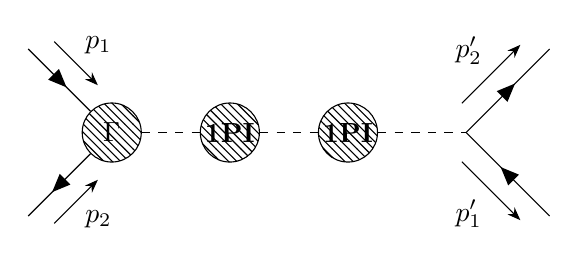
\begin{tikzpicture}[baseline = -0.11cm]
\begin{feynman}
\vertex [blob](a) {\(\Gamma\)};
\vertex [above left=of a, momentum = $p_1$] (i1) ;
\vertex [below left=of a, rmomentum = $p_2$] (i2) ;
\vertex [right=of a, blob] (b) {\(\mathbf{1PI}\)};
\vertex [right=of b, blob] (c) {\(\mathbf{1PI}\)};
\vertex [right=of c] (d);
\vertex [above right=of d] (f1) ;
\vertex [below right=of d] (f2) ;
\diagram* {
(i1) --[fermion, momentum = $p_1$] (a) -- [fermion, rmomentum = $p_2$] (i2),
(a) -- [scalar] (b) -- [scalar] (c) -- [scalar] (d),
(f2) --[fermion, rmomentum = $p_1'$] (d) -- [fermion, momentum = $p_2'$] (f1)
};
\end{feynman}
\end{tikzpicture}
\end{equation*}
\begin{equation*}
\quad 
+
\quad 
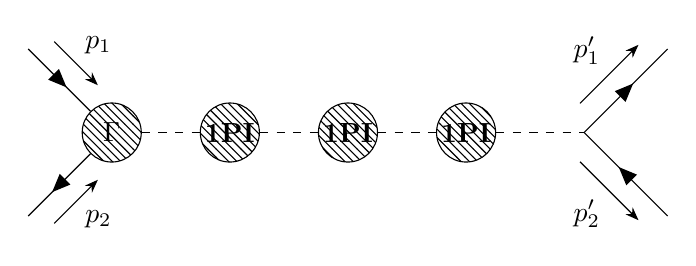
\begin{tikzpicture}[baseline = -0.11cm]
\begin{feynman}
\vertex [blob](a) {\(\Gamma\)};
\vertex [above left=of a] (i1) ;
\vertex [below left=of a] (i2) ;
\vertex [right=of a, blob] (b) {\(\mathbf{1PI}\)};
\vertex [right=of b, blob] (c) {\(\mathbf{1PI}\)};
\vertex [right=of c, blob] (d) {\(\mathbf{1PI}\)};
\vertex [right=of d] (e);
\vertex [above right=of e] (f1) ;
\vertex [below right=of e] (f2) ;
\diagram* {
(i1) --[fermion, momentum = $p_1$] (a) -- [fermion, rmomentum = $p_2$] (i2),
(a) -- [scalar] (b) -- [scalar] (c) -- [scalar] (d) -- [scalar] (e),
(f2) --[fermion, rmomentum = $p_2'$] (e) -- [fermion, momentum = $p_1'$] (f1)
};
\end{feynman}
\end{tikzpicture}
\quad
+ 
\quad
\cdots
\end{equation*}
and similarly,
\begin{equation*}
\begin{tikzpicture}[baseline = -1.7cm]
\begin{feynman}
\vertex [blob](a) {\(\Gamma\)};
\vertex [above left=of a, momentum' = $p_1$] (i1) ;
\vertex [above right=of a, rmomentum = $p_2$] (i2) 
;
\vertex [below=of a, blob] (b) {\(\mathbf{1PI}\)};
\vertex [below=of b] (c);
\vertex [below left=of c] (f1) ;
\vertex [below right=of c] (f2) ;
\diagram* {
(i1) --[fermion, momentum' = $p_1$] (a) -- [fermion, momentum' = $p_1'$] (i2),
(a) -- [scalar] (b) -- [scalar] (c)
(f2) --[fermion, rmomentum' = $p_2'$] (c) -- [fermion, rmomentum' = $p_2$] (f1)
};
\end{feynman}
\end{tikzpicture}
\quad 
+
\quad 
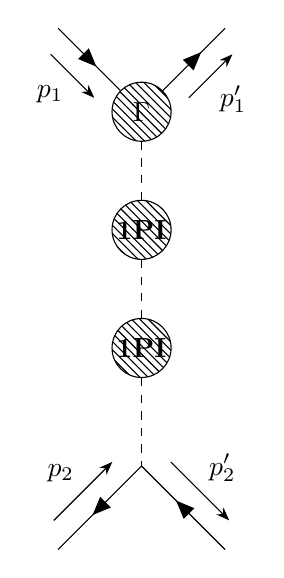
\begin{tikzpicture}[baseline = -2.5cm]
\begin{feynman}
\vertex [blob](a) {\(\Gamma\)};
\vertex [above left=of a, momentum' = $p_1$] (i1) ;
\vertex [above right=of a, rmomentum = $p_2$] (i2) 
;
\vertex [below=of a, blob] (b) {\(\mathbf{1PI}\)};
\vertex [below=of b, blob] (c) {\(\mathbf{1PI}\)};
\vertex [below=of c] (d);
\vertex [below left=of d] (f1) ;
\vertex [below right=of d] (f2) ;
\diagram* {
(i1) --[fermion, momentum' = $p_1$] (a) -- [fermion, momentum' = $p_1'$] (i2),
(a) -- [scalar] (b) -- [scalar] (c) -- [scalar] (d),
(f2) --[fermion, rmomentum' = $p_2'$] (d) -- [fermion, rmomentum' = $p_2$] (f1)
};
\end{feynman}
\end{tikzpicture}
\quad 
+
\quad 
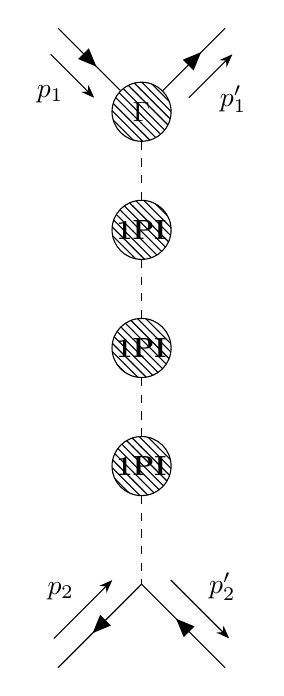
\begin{tikzpicture}[baseline = -3cm]
\begin{feynman}
\vertex [blob](a) {\(\Gamma\)};
\vertex [above left=of a, momentum' = $p_1$] (i1) ;
\vertex [above right=of a, rmomentum = $p_2$] (i2) 
;
\vertex [below=of a, blob] (b) {\(\mathbf{1PI}\)};
\vertex [below=of b, blob] (c) {\(\mathbf{1PI}\)};
\vertex [below=of c, blob] (d) {\(\mathbf{1PI}\)};
\vertex [below=of d] (e);
\vertex [below left=of e] (f1) ;
\vertex [below right=of e] (f2) ;
\diagram* {
(i1) --[fermion, momentum' = $p_1$] (a) -- [fermion, momentum' = $p_1'$] (i2),
(a) -- [scalar] (b) -- [scalar] (c) -- [scalar] (d) -- [scalar] (e),
(f2) --[fermion, rmomentum' = $p_2'$] (e) -- [fermion, rmomentum' = $p_2$] (f1)
};
\end{feynman}
\end{tikzpicture}
\quad
+ 
\quad
\cdots
\end{equation*}
and likewise flipped diagrams.
These corrections are at a higher order than the level of perturbation theory we are considering so there is no mystery in the fact that none of the these diagrams contributing to the expression with the full propagator appeared in our analysis.
Consider the real and imaginary parts of the propagator,
\begin{align*}
\tilde{G}^{(2)}(p) = \frac{i}{p^2 - m^2 - \mathrm{Re}[\Sigma(p^2)] - i \mathrm{Im}[\Sigma(p^2)]} = \frac{i(p^2 - m^2 - \mathrm{Re}[\Sigma(p^2)] + i \mathrm{Im}[\Sigma(p^2)])}{(p^2 - m^2 - \mathrm{Re}[\Sigma(p^2)])^2 + \mathrm{Im}[\Sigma(p^2)]^2}
\end{align*}
Therefore, at the resonant mass $p^2 = m^2$, since the renormalization condition implies $\mathrm{Re}[\Sigma(p^2 = m^2)] = 0$ then,
\[ \tilde{G}^{(2)}(p^2 = m^2) = - \frac{1}{\mathrm{Im}[\Sigma(m^2)]} = \frac{1}{m \Gamma} \]
Therefore, $\Gamma^{-1}$ measures the height of the resonant peak, $2 \Gamma$ measures the full width at half max of the resonant peak, and $\Gamma^{-1}$ gives the lifetime of the unstable particle.
Using this notation, the scattering cross section becomes, 
\begin{align*}
\deriv{\sigma}{\Omega} 
&= \frac{g^4}{64 \pi^2 s} \left| \frac{1 + 2\tilde{\Gamma}(t)}{t - m^2 - \Sigma_\phi(t)} + \frac{1 + 2\tilde{\Gamma}(s)}{s - m^2 - \Sigma_\phi(s)} + B(t, s) + B(s, t) + B(u, s) + B(u, t)  \right|^2 
\end{align*}

\subsection{Explicit Evaluation of the Scattering Cross Section}

\subsubsection{Scattering in the Stable Meson Regime: $m < 2 M$}
Throughout this section, we will quote results for the case, $m = 0.5M$ and $g = 0.25$ in which the meson is stable. Results for the tree-level calculation which is accurate to order $g^4$ in the cross section and the one-loop calculation accurate to order $g^8$ in the cross section will be compared. In general, high energy scattering in enhanced at the one-loop level due to the contribution of the box diagrams, see figure \ref{StabHighEnergy}. The angular dependence of the scattering amplitude is presented as a magnitude-angle plot, see figure \ref{stable-angular}. which shows the dominance of forward scattering at high energy and little angular bias and low energy.

\begin{figure}
\begin{center}
\vspace*{-2cm}
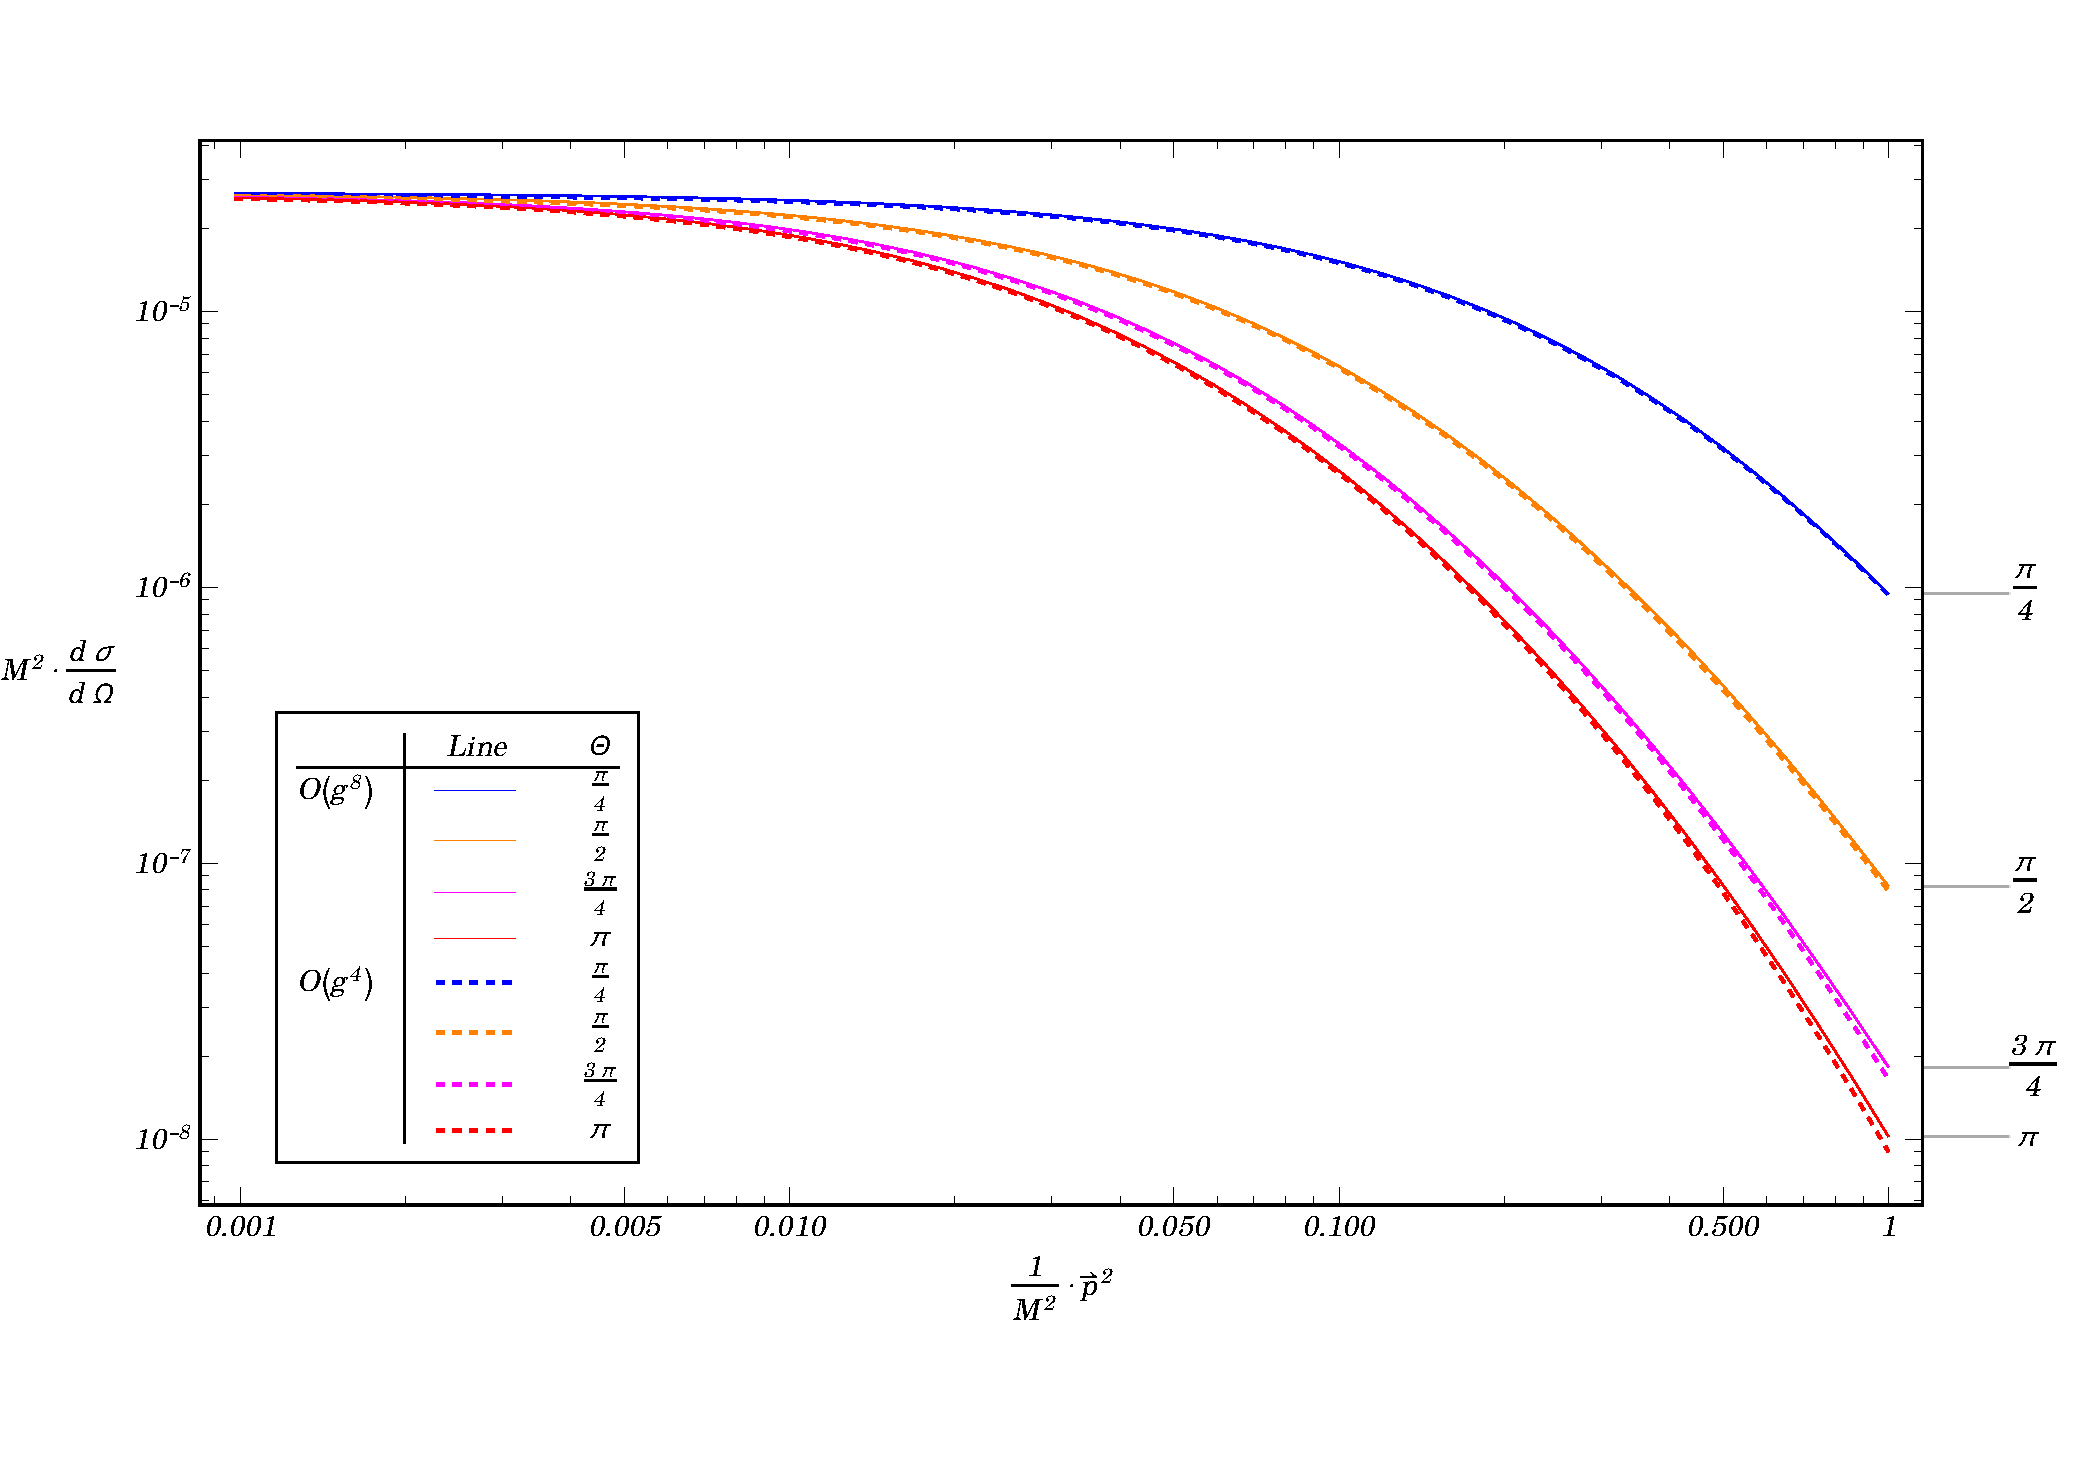
\includegraphics[width=15cm, height=11cm]{StableMeson-LowEnergy}
\caption{Low energy scattering cross section in the stable meson regime with parameters $m = 0.5 M$ and $g = 0.25$. The calculation is performed both at tree-level (dashed) in the cross section and the one-loop level (solid) in perturbation theory at four different fixed values for the scattering angle $\Theta$. The scale is log-log.} 
\label{StabLowEnergy}
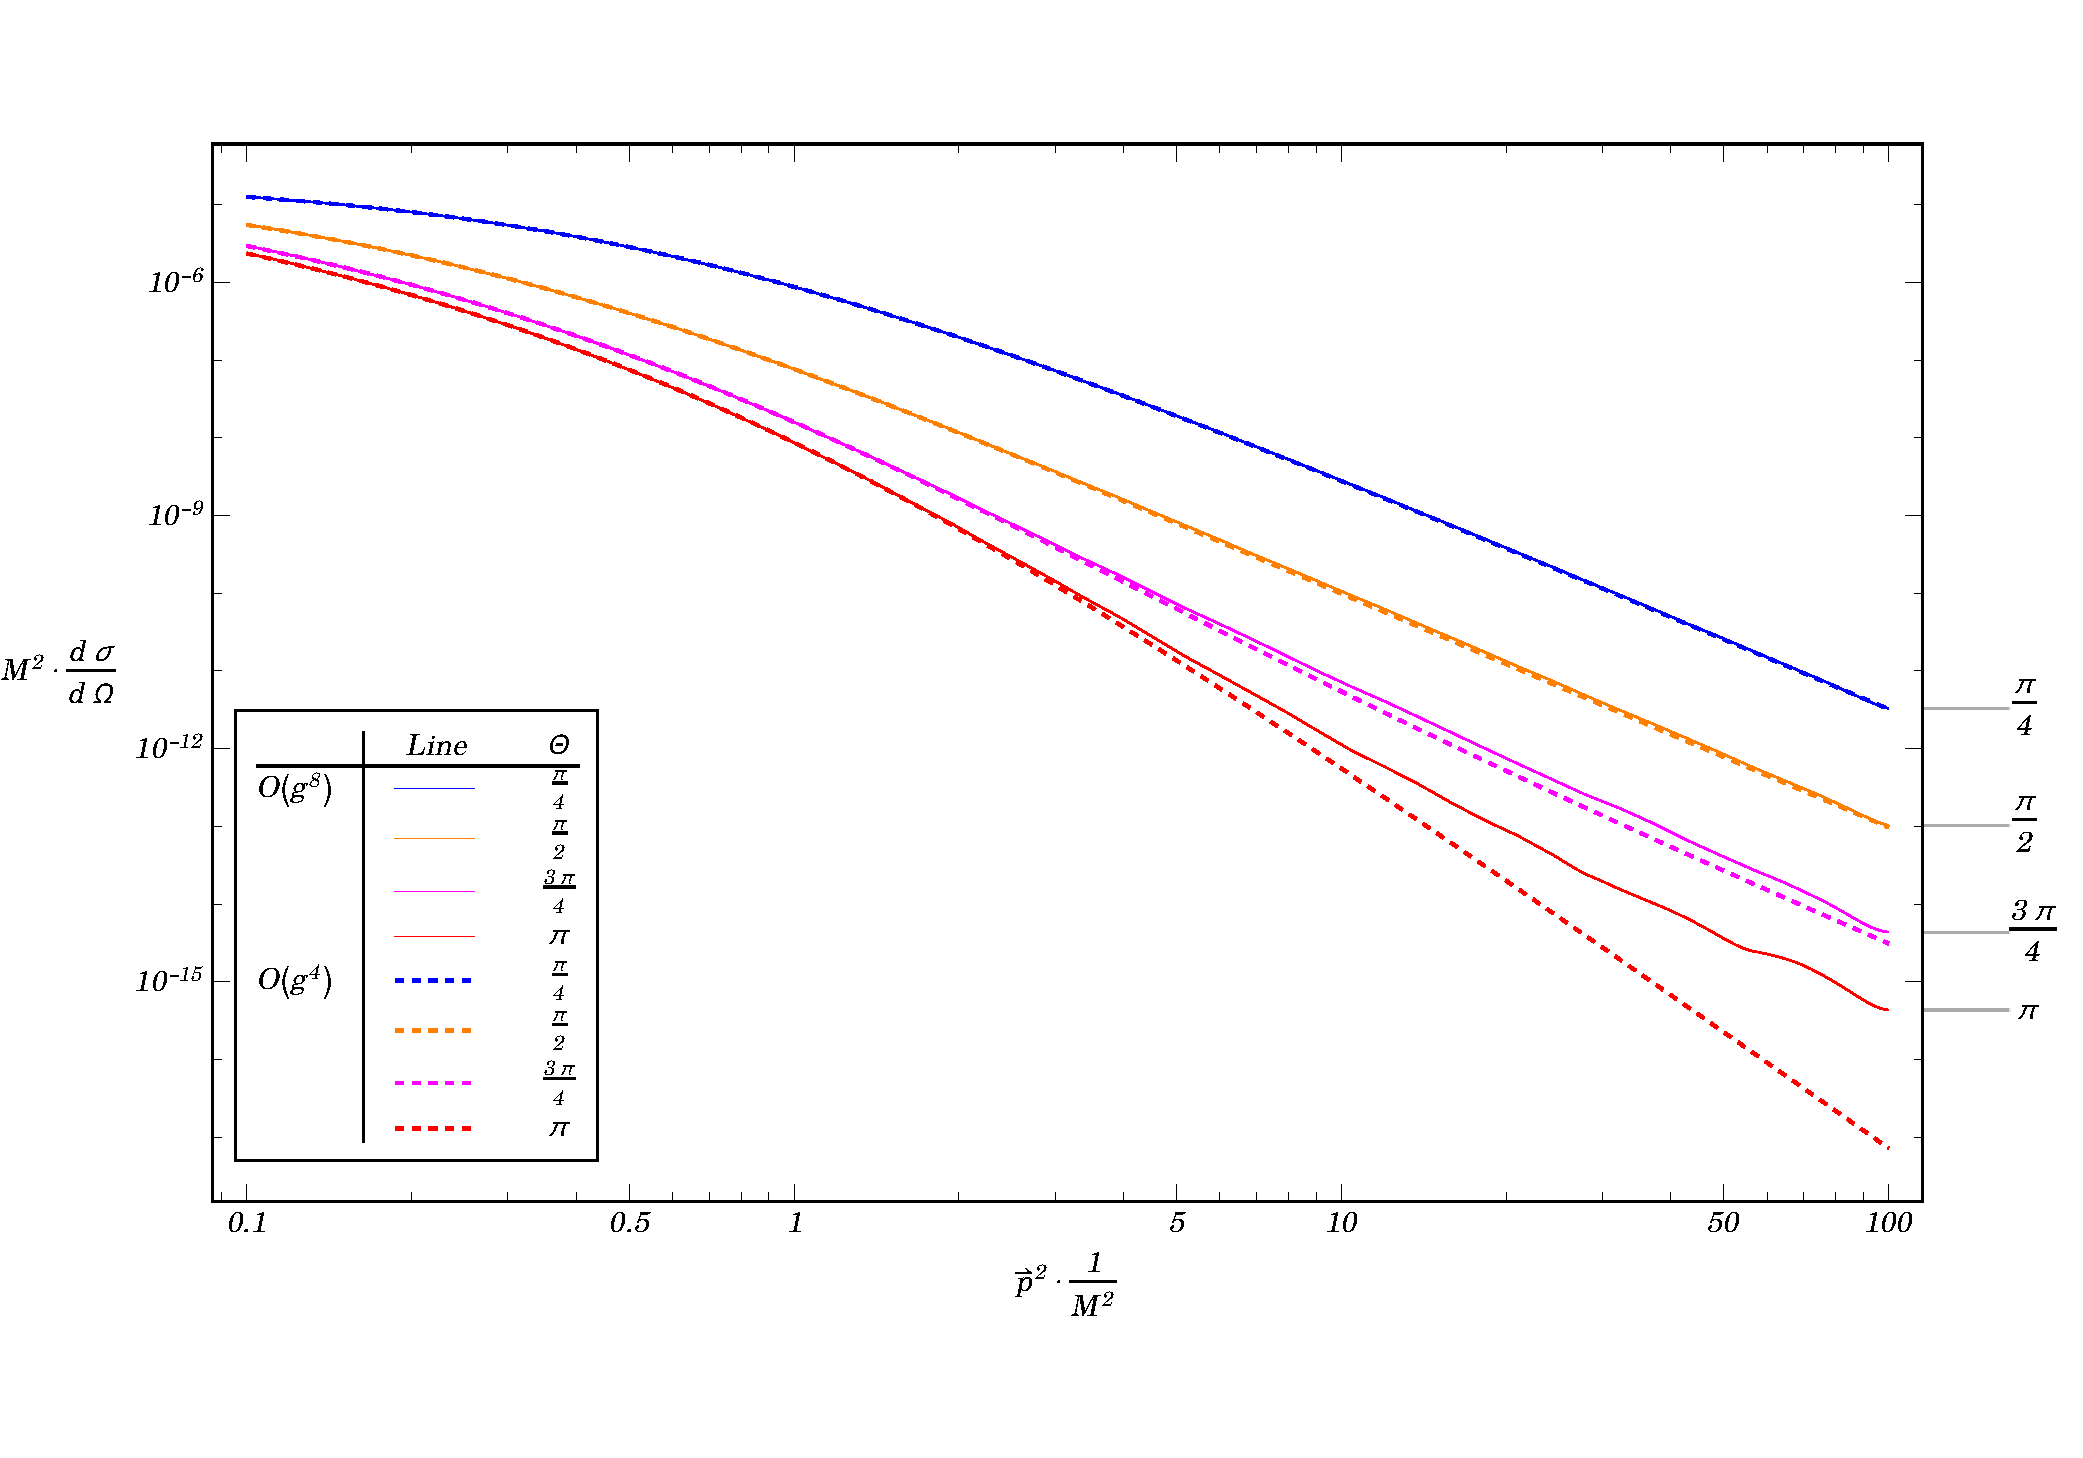
\includegraphics[width=15cm, height=11cm]{StableMeson-HighEnergy}
\caption{High energy scattering cross section in the stable meson regime with parameters $m = 0.5 M$ and $g = 0.25$. The calculation is performed both at tree-level (dashed) in the cross section and the one-loop level (solid) in perturbation theory at four different fixed values for the scattering angle $\Theta$. The scale is log-log.} 
\label{StabHighEnergy}
\end{center}
\end{figure} 


\begin{figure}
\begin{center}
\vspace*{-2cm}
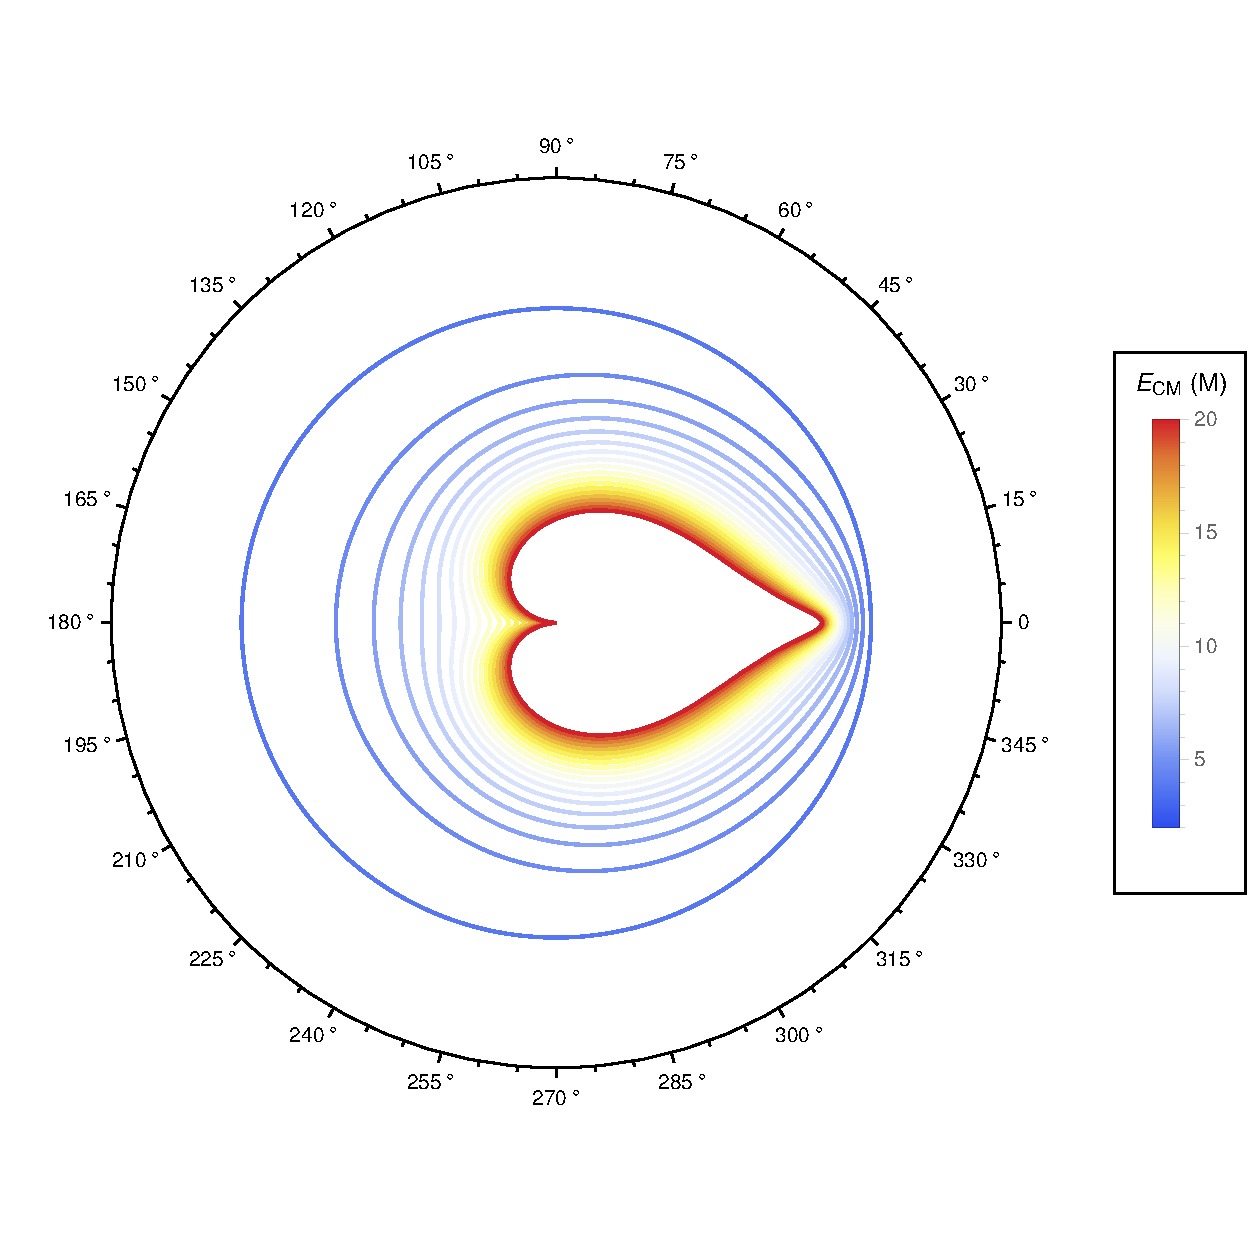
\includegraphics[width=14cm, height=14cm]{StableMeson-LowEnergy-Polar}
\caption{Angular dependence of the scattering cross section in the stable meson regime for $m = 0.5 M$. Scattering cross sections are plotted on a log scale. Total scattering energy is expressed in multiples of the $\psi$ rest mass.} 
\label{stable-angular}
\end{center}
\end{figure}

\subsubsection{Scattering in the Unstable Resonant Regime: $m > 2 M$}
When the meson becomes unstable, two new phenomena appear. When the total scattering energy equals the mass energy of the meson, a resonance in the scattering amplitude forms due to the creation of a semi-stable meson as an intermediate product in the process $\psi \bar{\psi} \to \phi \to \psi \bar{\psi}$. This resonance only appears in $s$-channel diagrams because it relies on the possibility of $\psi-\bar{\psi}$ annihilation. Along with resonances, anti-resonances appear in the scattering amplitude only in the regime $m > 2 M$. At an anti-resonance, the scattering amplitude drops nearly (at tree-level exactly) to zero due to destructive interference between the $s$ and $t$-channel amplitudes. At a fixed energy, the destructive interference only occurs for a fixed scattering angle $\Theta$. Figure \ref{unstable-angular}. shows how the position of the anti-resonance shifts towards back-scattering in the high energy limit. For exact back-scattering or forward-scattering, no anti-resonance occurs. However, at any other fixed scattering angle there is a particular total energy at which the destructive interference occurs in that direction.\bigskip\\
The imaginary part of the dressed propagator for $\phi$ smooths both the resonances and anti-resonances such that the scattering amplitude does not have poles or zeros for physical scattering energies. Furthermore, the contribution of box diagrams shifts the location of the destructive interference and somewhat softens the cusp (see figure \ref{AntiResonance}.) The quadratic nature of these anti-resonances due to destructive interference can be seen when the amplitude is viewed on a linear scale as in figure \ref{NoLogAntiResonance}.    


\begin{figure}
\begin{center}
\vspace*{-2cm}
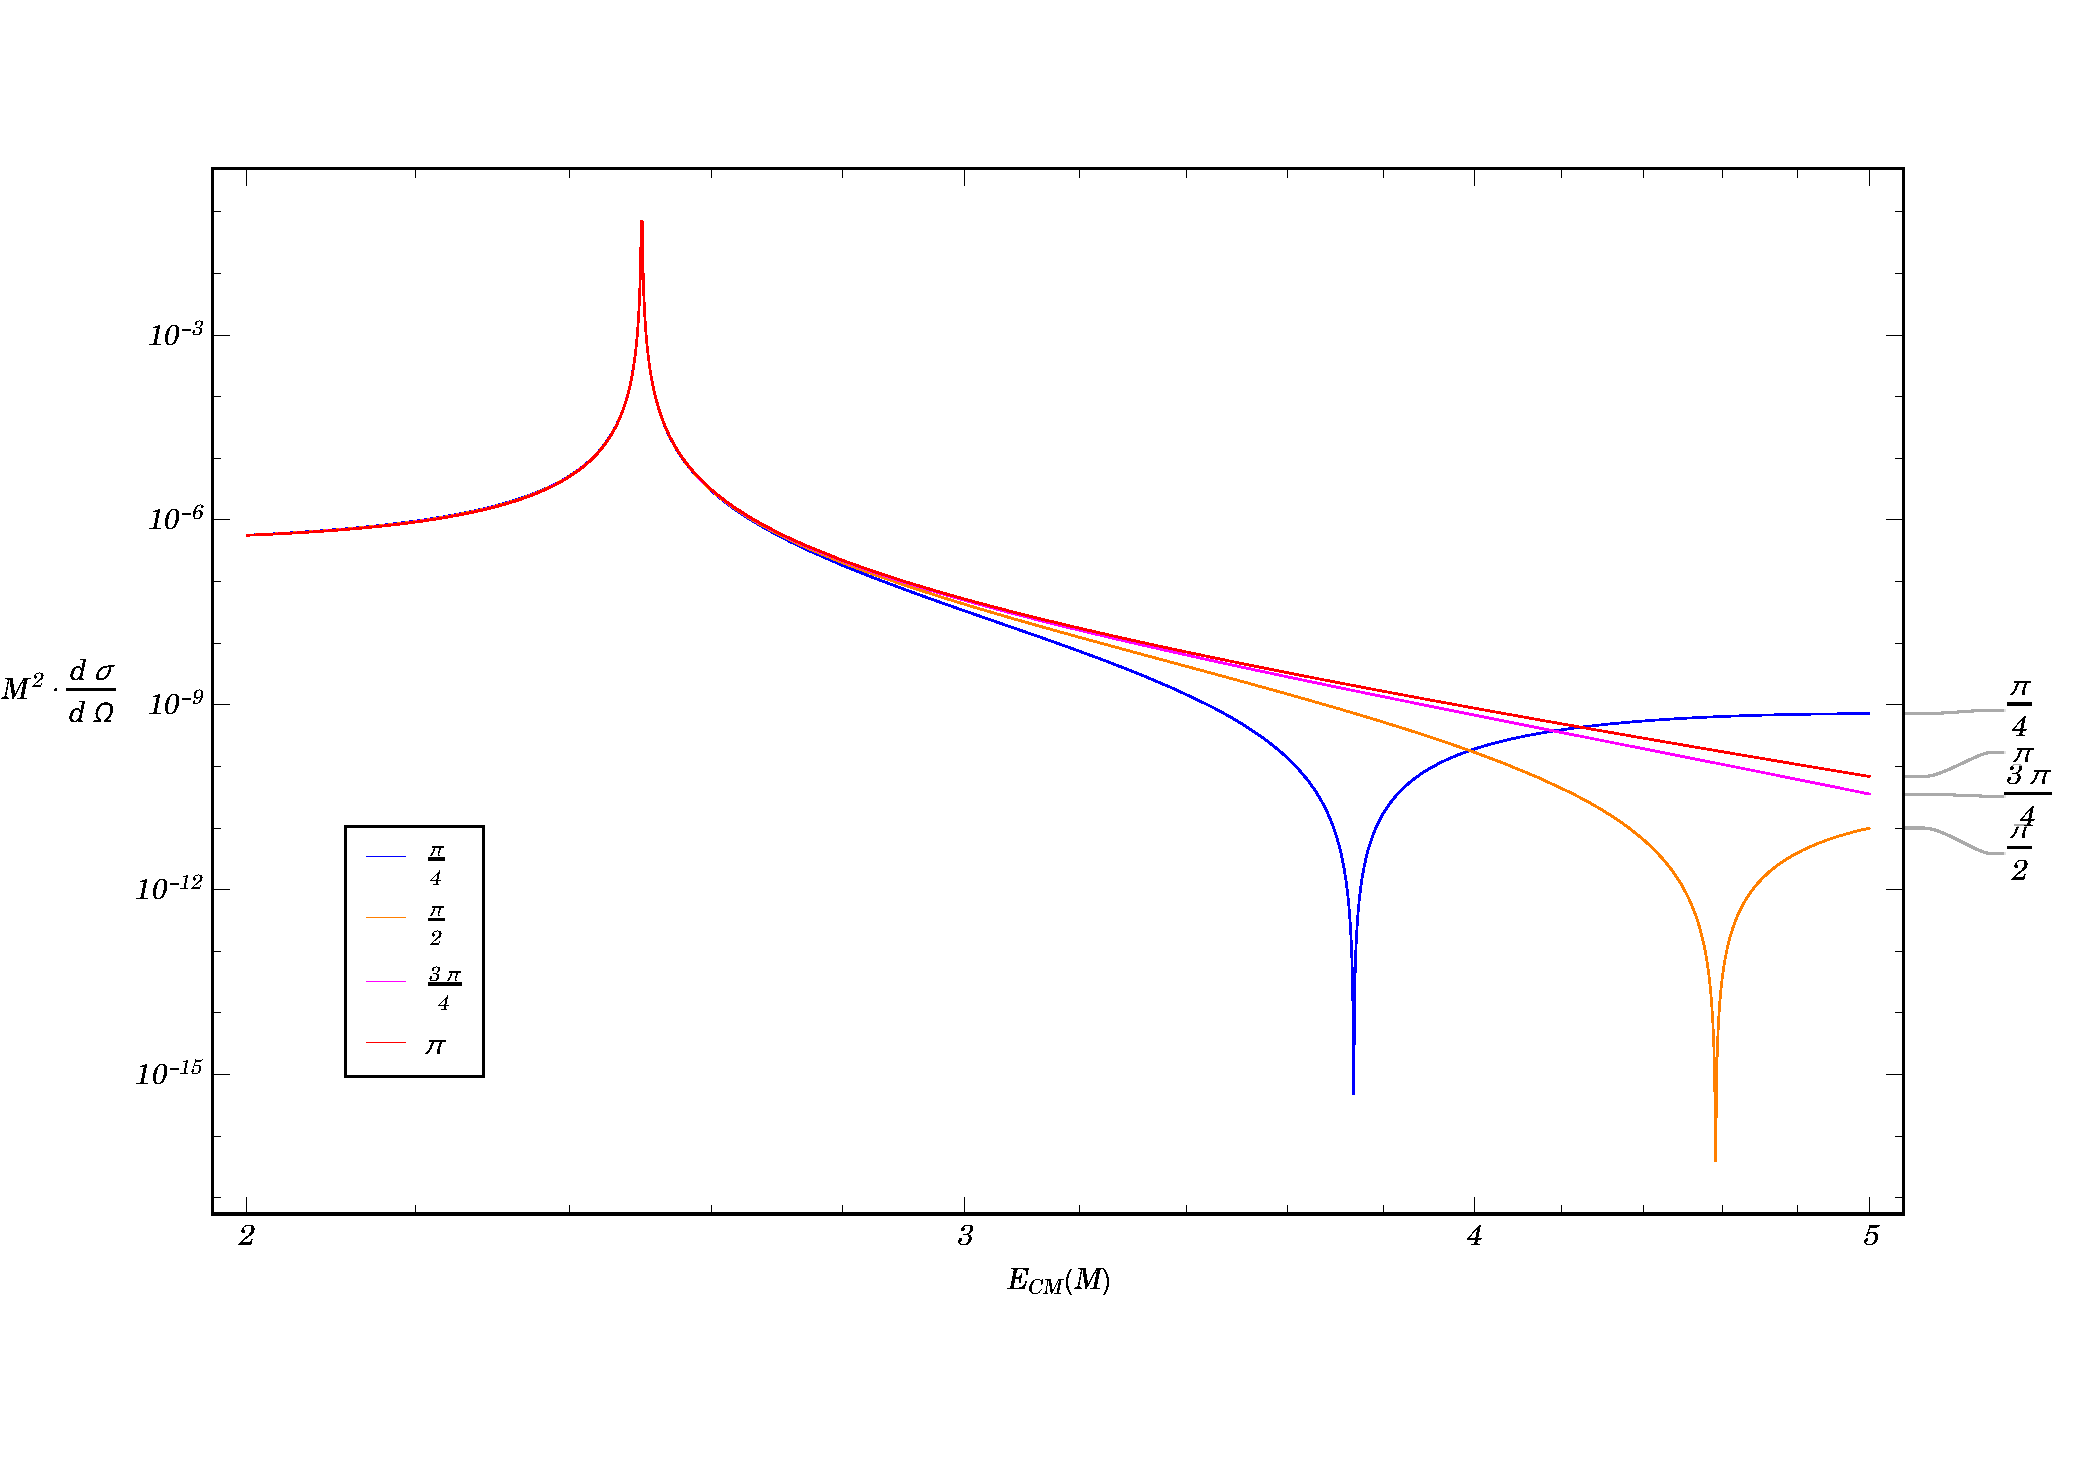
\includegraphics[width=15cm, height=11cm]{UnStableMeson-LowEnergy}
\caption{Low energy scattering cross section in the unstable meson regime with parameters $m = 2.5 M$ and $g = 0.25$. The calculation is performed both at tree-level (dashed) in the cross section and the one-loop level (solid) in perturbation theory at four different fixed values for the scattering angle $\Theta$. The scale is log-log.} 
\label{UnStabLowEnergy}
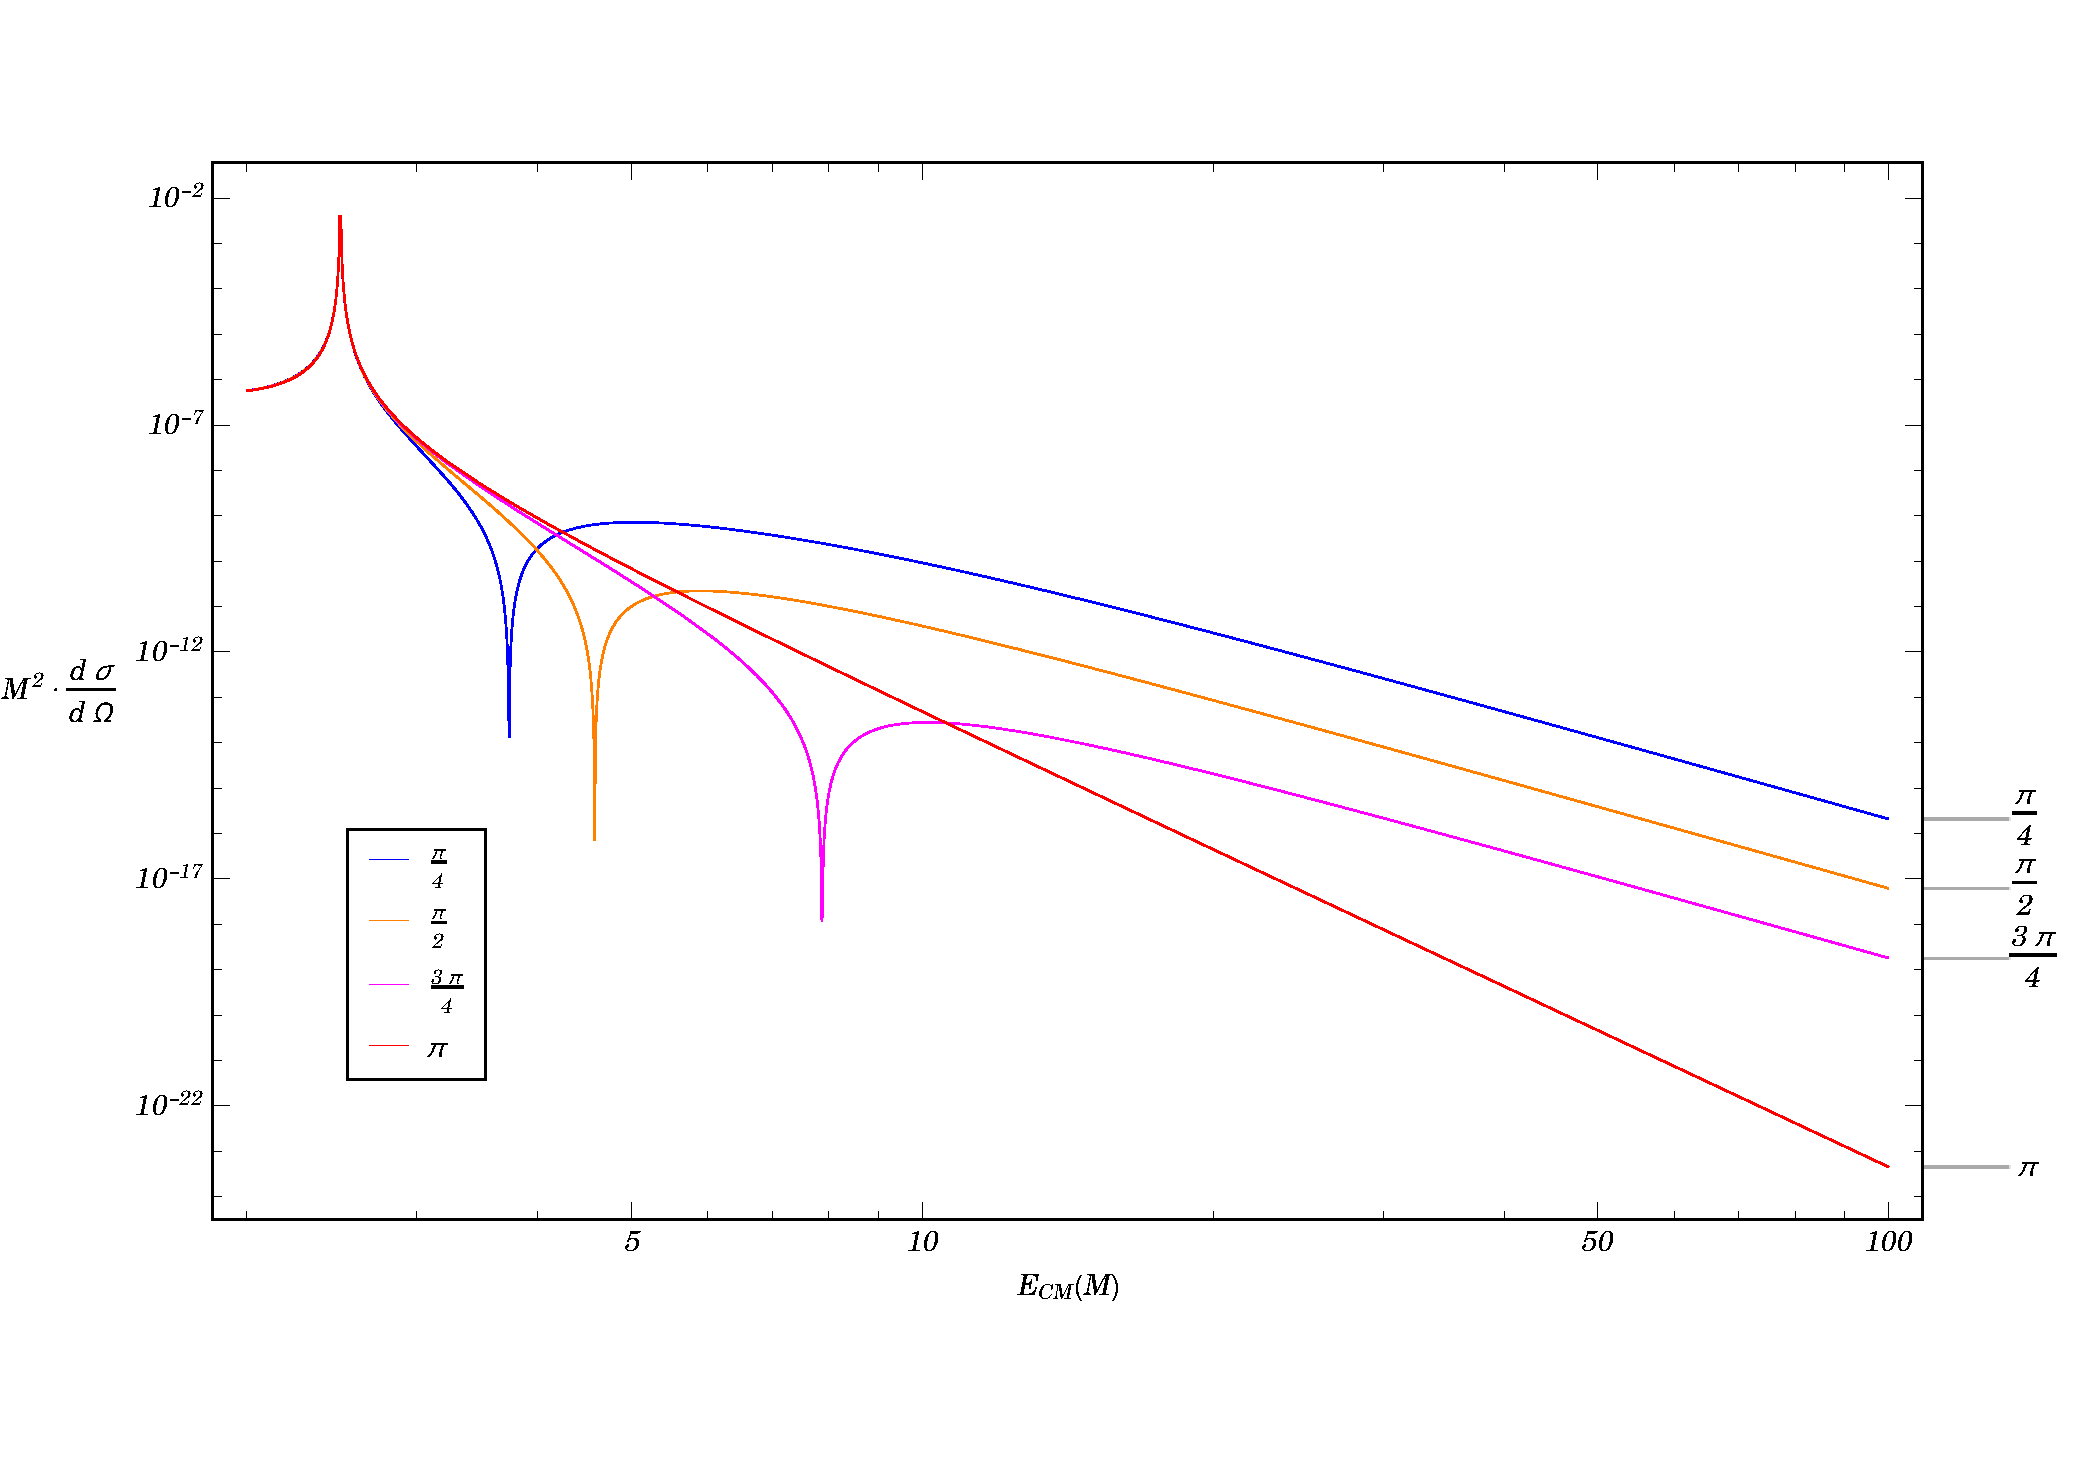
\includegraphics[width=15cm, height=11cm]{UnStableMeson-HighEnergy}
\caption{High energy scattering cross section in the unstable meson regime with parameters $m = 2.5 M$ and $g = 0.25$. The calculation is performed both at tree-level (dashed) in the cross section and the one-loop level (solid) in perturbation theory at four different fixed values for the scattering angle $\Theta$. The scale is log-log. Energies are expressed in multiples of the $\psi$ particle rest mass.} 
\label{UnStabHighEnergy}
\end{center}
\end{figure} 

\begin{figure}
\begin{center}
\vspace*{-2.5cm}
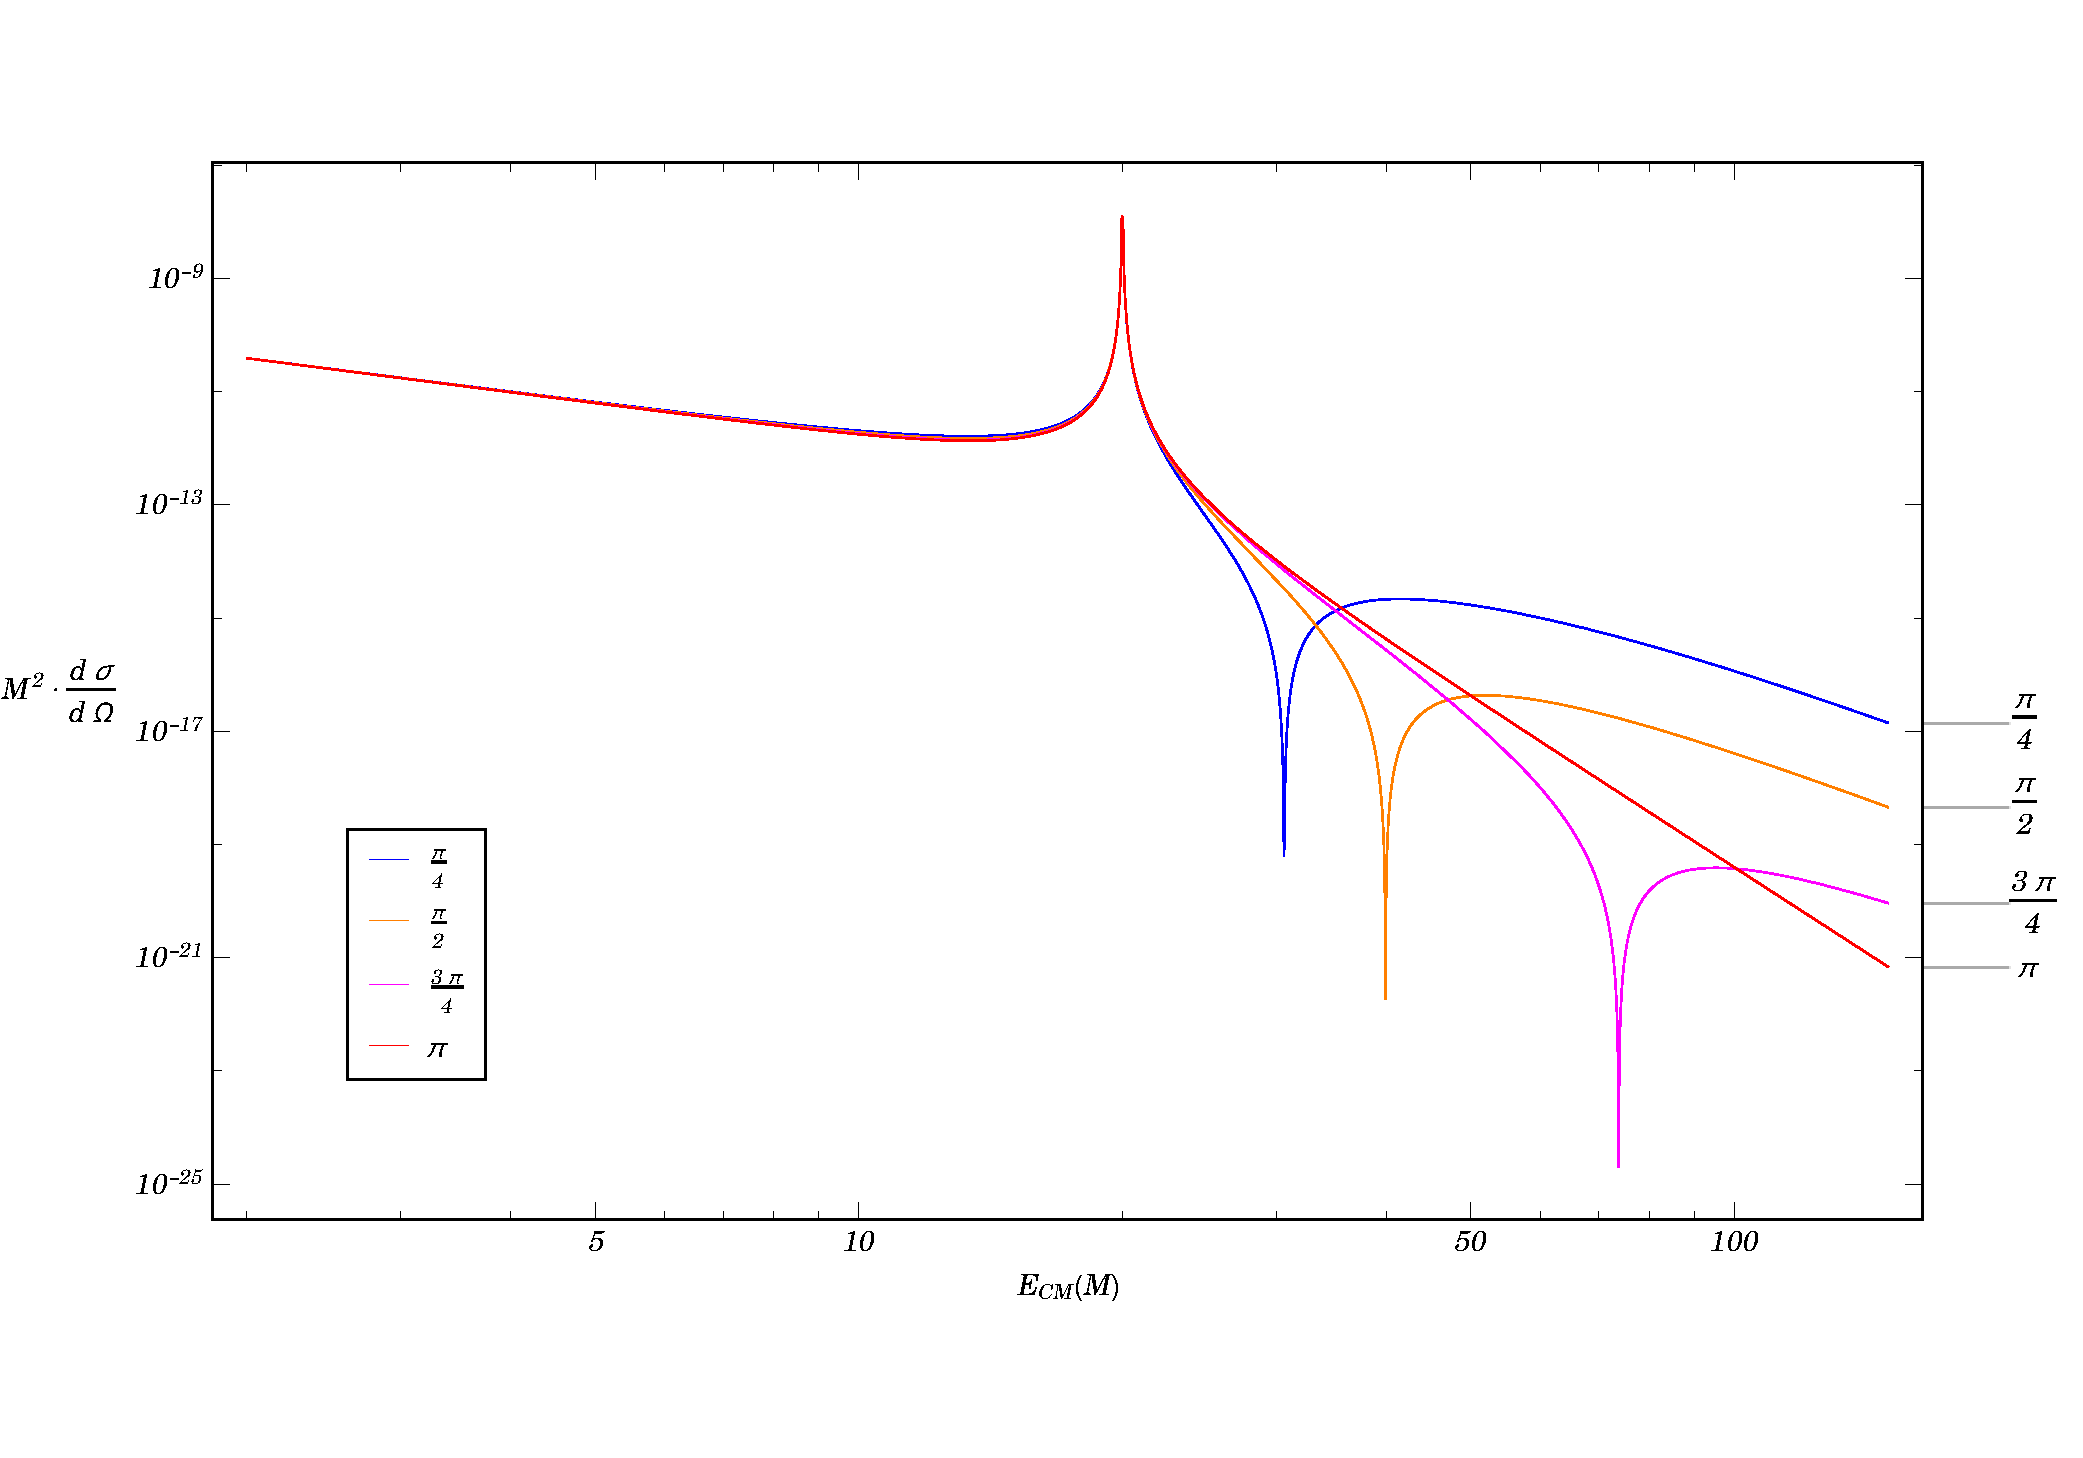
\includegraphics[width=15cm, height=11cm]{HighMass-UnStableMeson-HighEnergy}
\vspace*{-0.5cm}
\caption{Low energy scattering cross section for heavy mesons with parameters $m = 20 M$ and $g = 0.25$. The calculation is performed both at tree-level (dashed) in the cross section and the one-loop level (solid) in perturbation theory at four different fixed values for the scattering angle $\Theta$. The scale is log-log. Energies are expressed in multiples of the $\psi$ particle rest mass.} 
\label{HighMassUnStabHighEnergy}
\vspace*{-0.5cm}
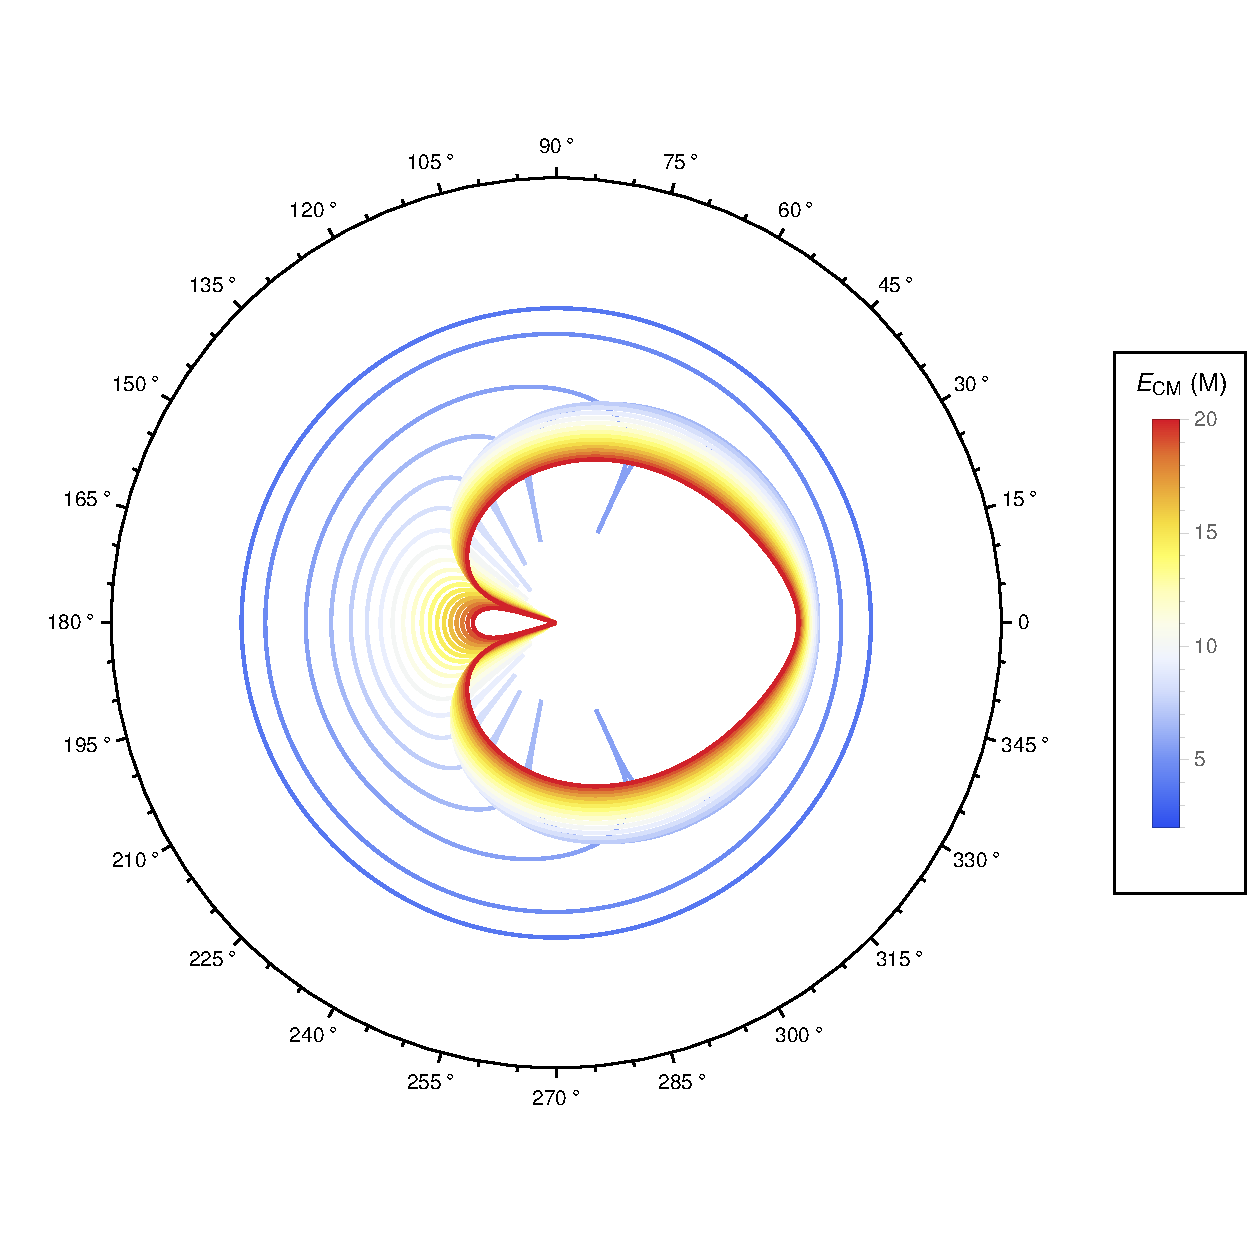
\includegraphics[width=14cm, height=14cm]{UnStableMeson-LowEnergy-Polar}
\vspace*{-1cm}
\caption{Angular dependence of the scattering cross section in the unstable meson regime with $m = 2.5 M$. Scattering cross sections are plotted on a log scale. Total scattering energy is expressed in multiples of the $\psi$ rest mass.} 
\label{unstable-angular}
\end{center}
\end{figure} 


\begin{figure}
\begin{center}
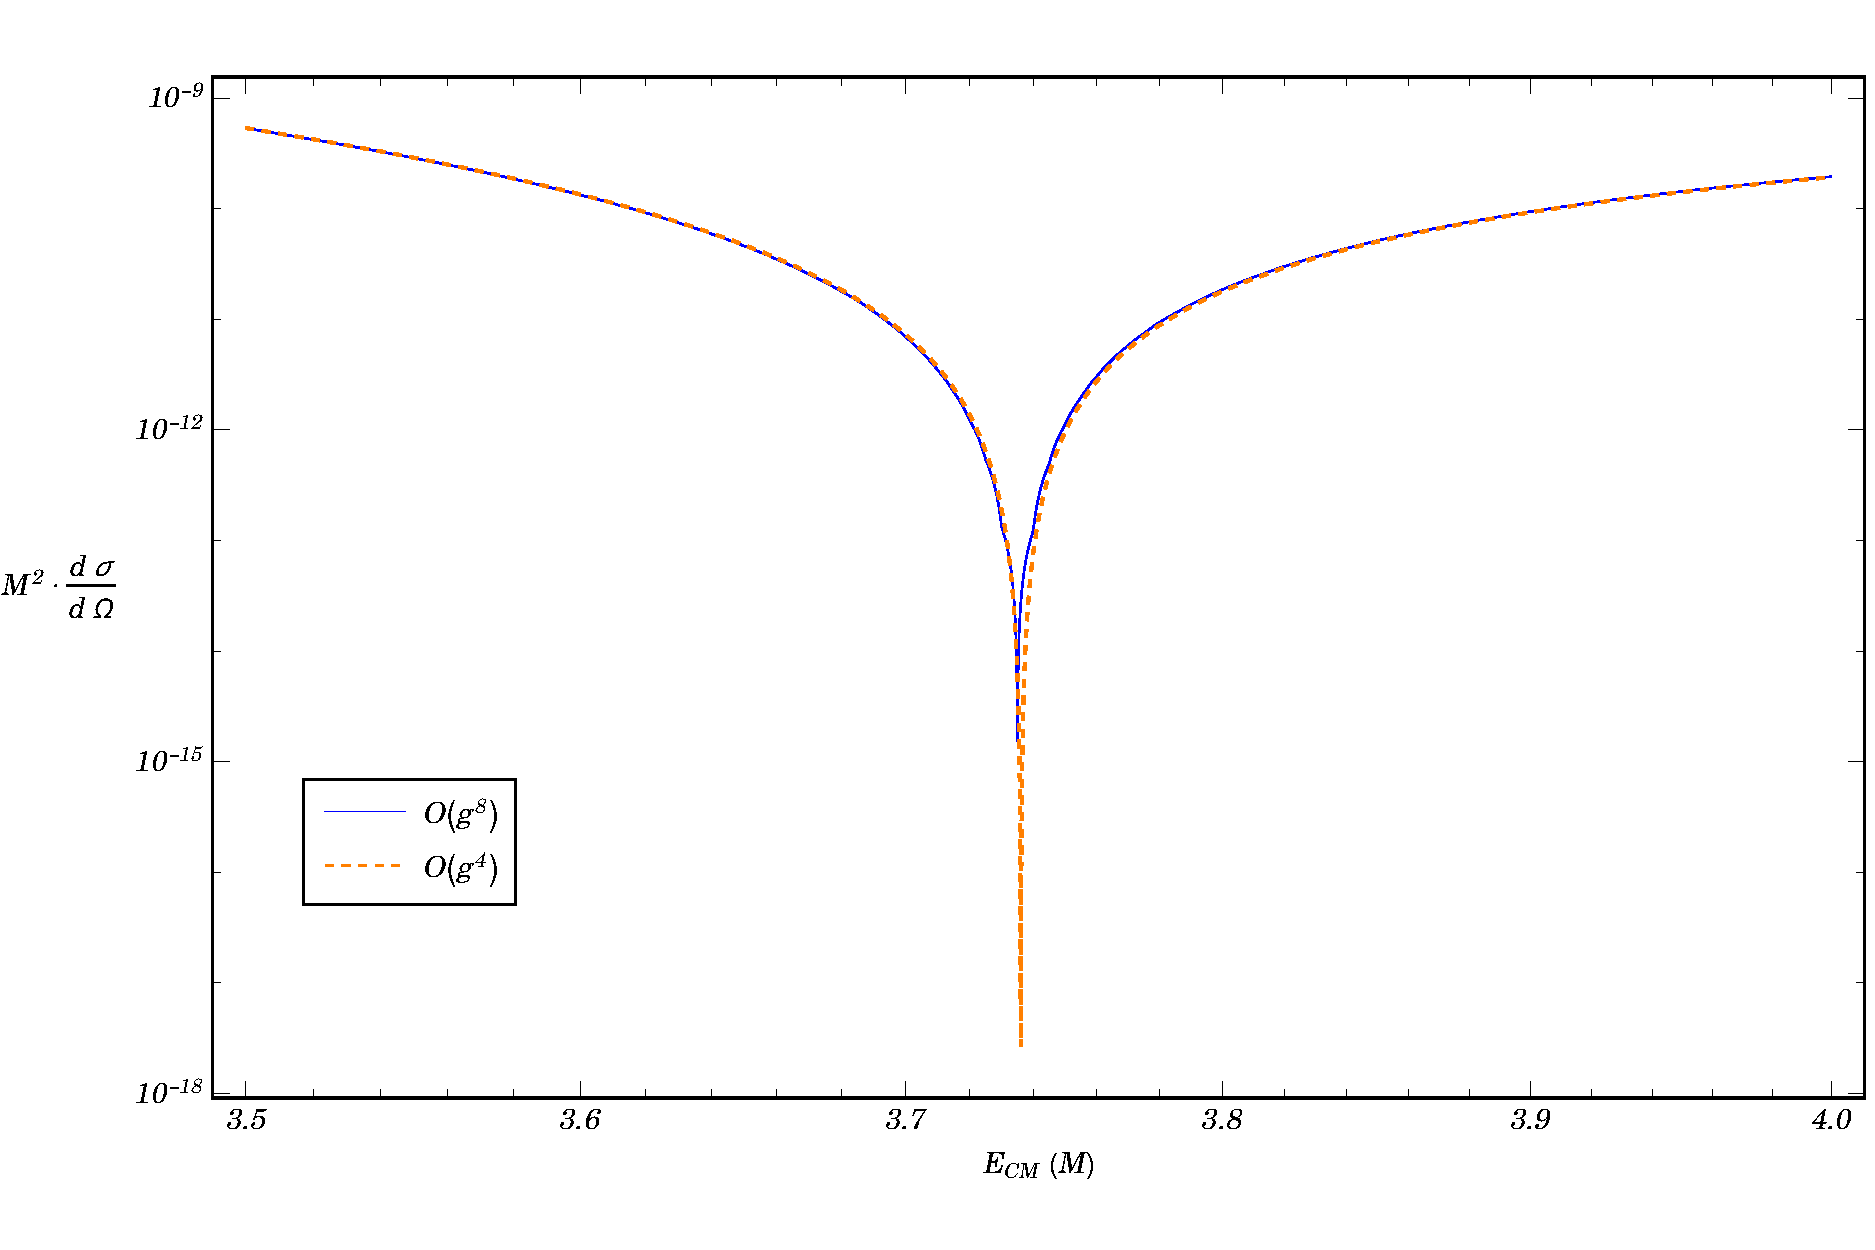
\includegraphics[width=15cm, height=10cm]{AntiResonance}
\caption{Closeup of destructive interference of the cross section at a fixed scattering angle in the unstable meson regime with $m = 2.5 M$ and $\Theta = \frac{\pi}{4}$. Scattering cross sections are plotted on a log scale. Total scattering energy is expressed in multiples of the $\psi$ rest mass.} 
\label{AntiResonance}
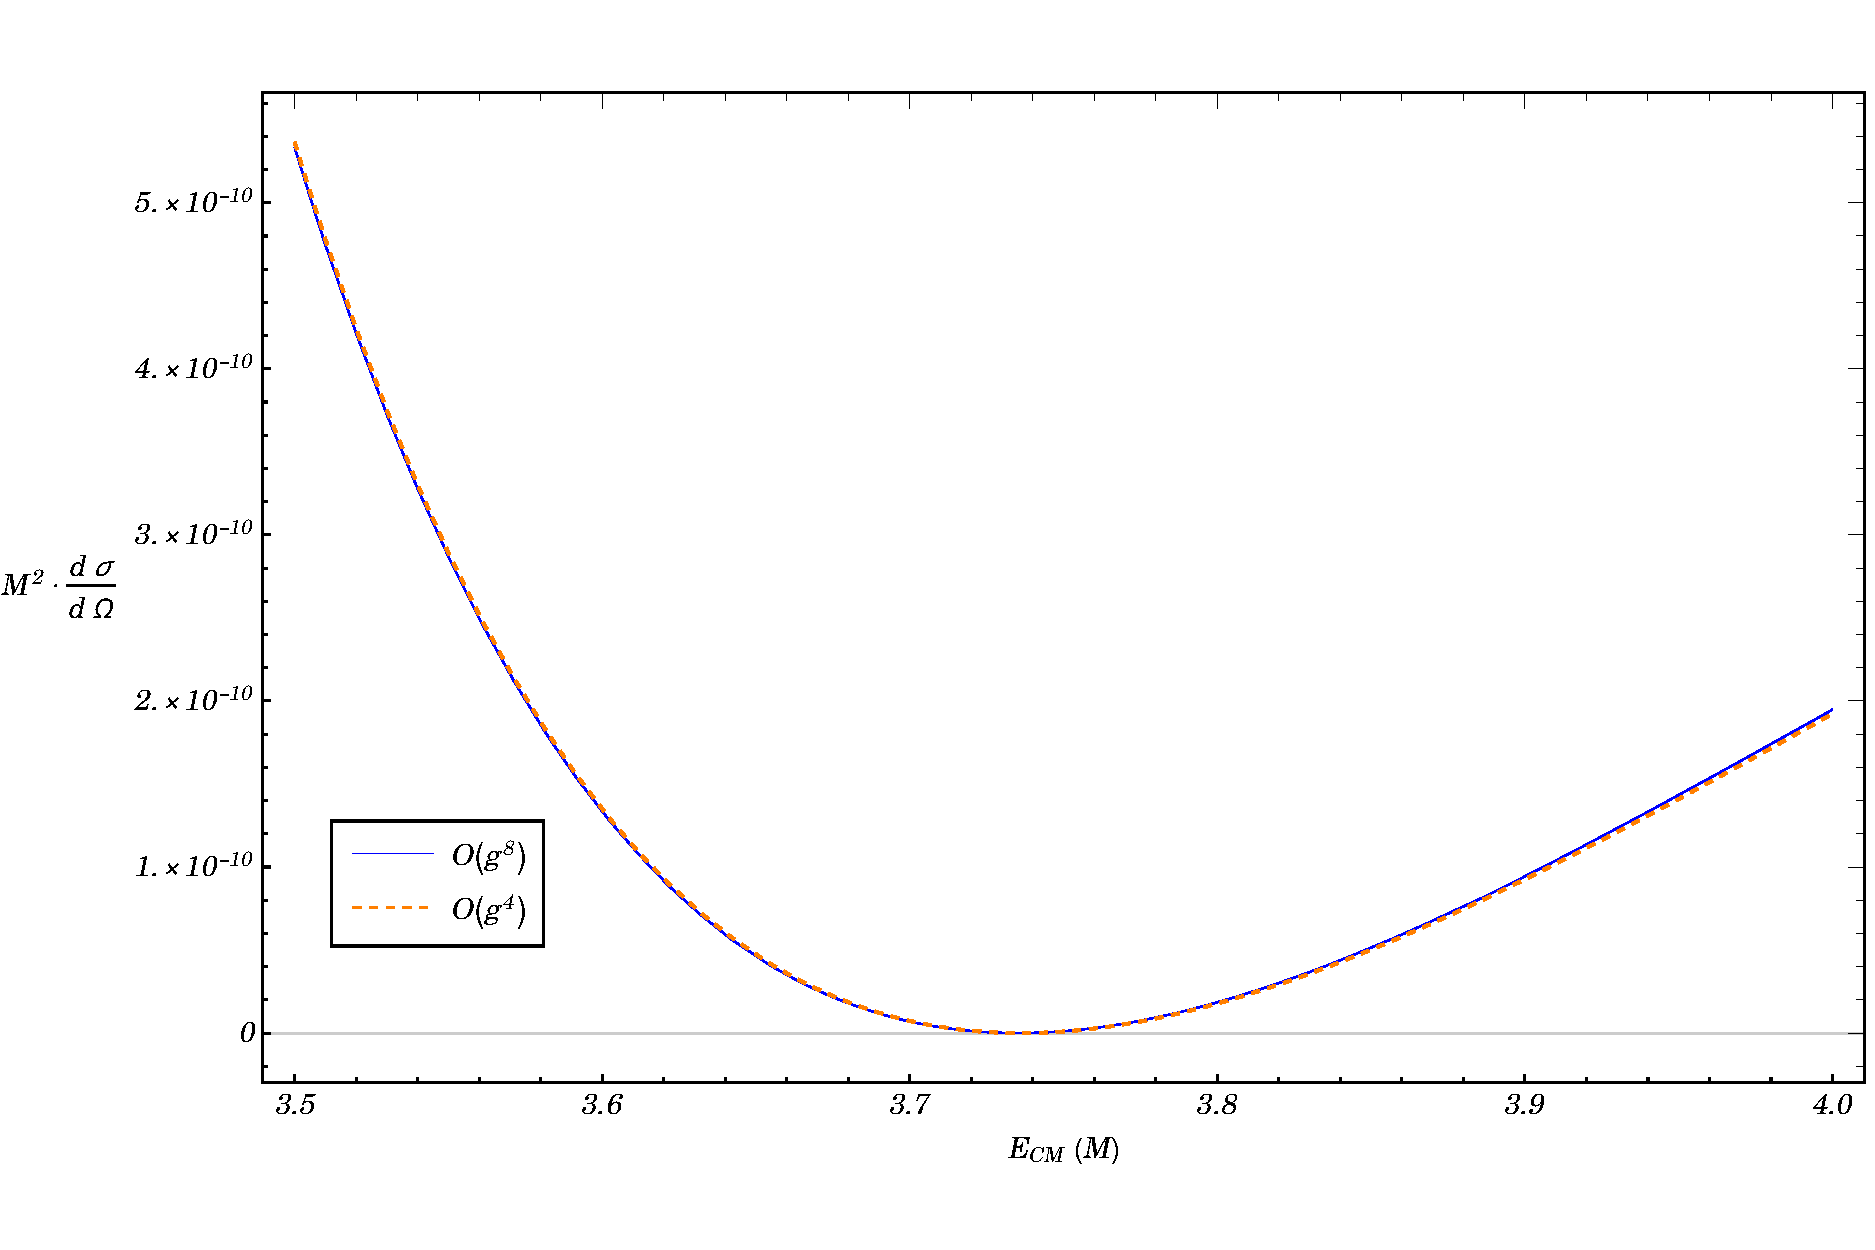
\includegraphics[width=15cm, height=10cm]{NoLogAntiResonance}
\caption{Closeup of destructive interference of the cross section at a fixed scattering angle in the unstable meson regime with $m = 2.5 M$ and $\Theta = \frac{\pi}{4}$. Scattering cross sections are plotted on a linear scale. Total scattering energy is expressed in multiples of the $\psi$ rest mass.} 
\label{NoLogAntiResonance}
\end{center}
\end{figure}

\subsubsection{Illustration of Scattering Resonance}
Even in the regime in which the meson is unstable, the interaction is weak enough that the meson is quite long-lived and therefore the scattering resonance is extremely sharp. To illustrate the appearance of a Breit-Winger distribution in the scattering amplitude due to resonances of unstable particles we employ an toy model of the toy scalar Yukawa theory. To do this, I will set $g = 4 M$ so we are far into the unpertubative regime in which our truncation of the Dyson series is not particularly well justified. That said, our truncated scattering amplitude is illustrative of resonance peaks in strongly coupled theories with highly unstable particles. In particular, as shown in figure \ref{Ill}. the full meson propagator has an imaginary part due to allowed decay channels which reduces the sharpness of the resonant peak. Similarly, the full propagator has the effect of shifting the energy (at a fixed scattering angle) at which destructive interference between the $s$ and $t$-channels occurs. Furthermore, the imaginary part of the propagator also obstructs the scattering amplitude from reaching zero at the point of destructive interference.     
\begin{figure}
\begin{center}
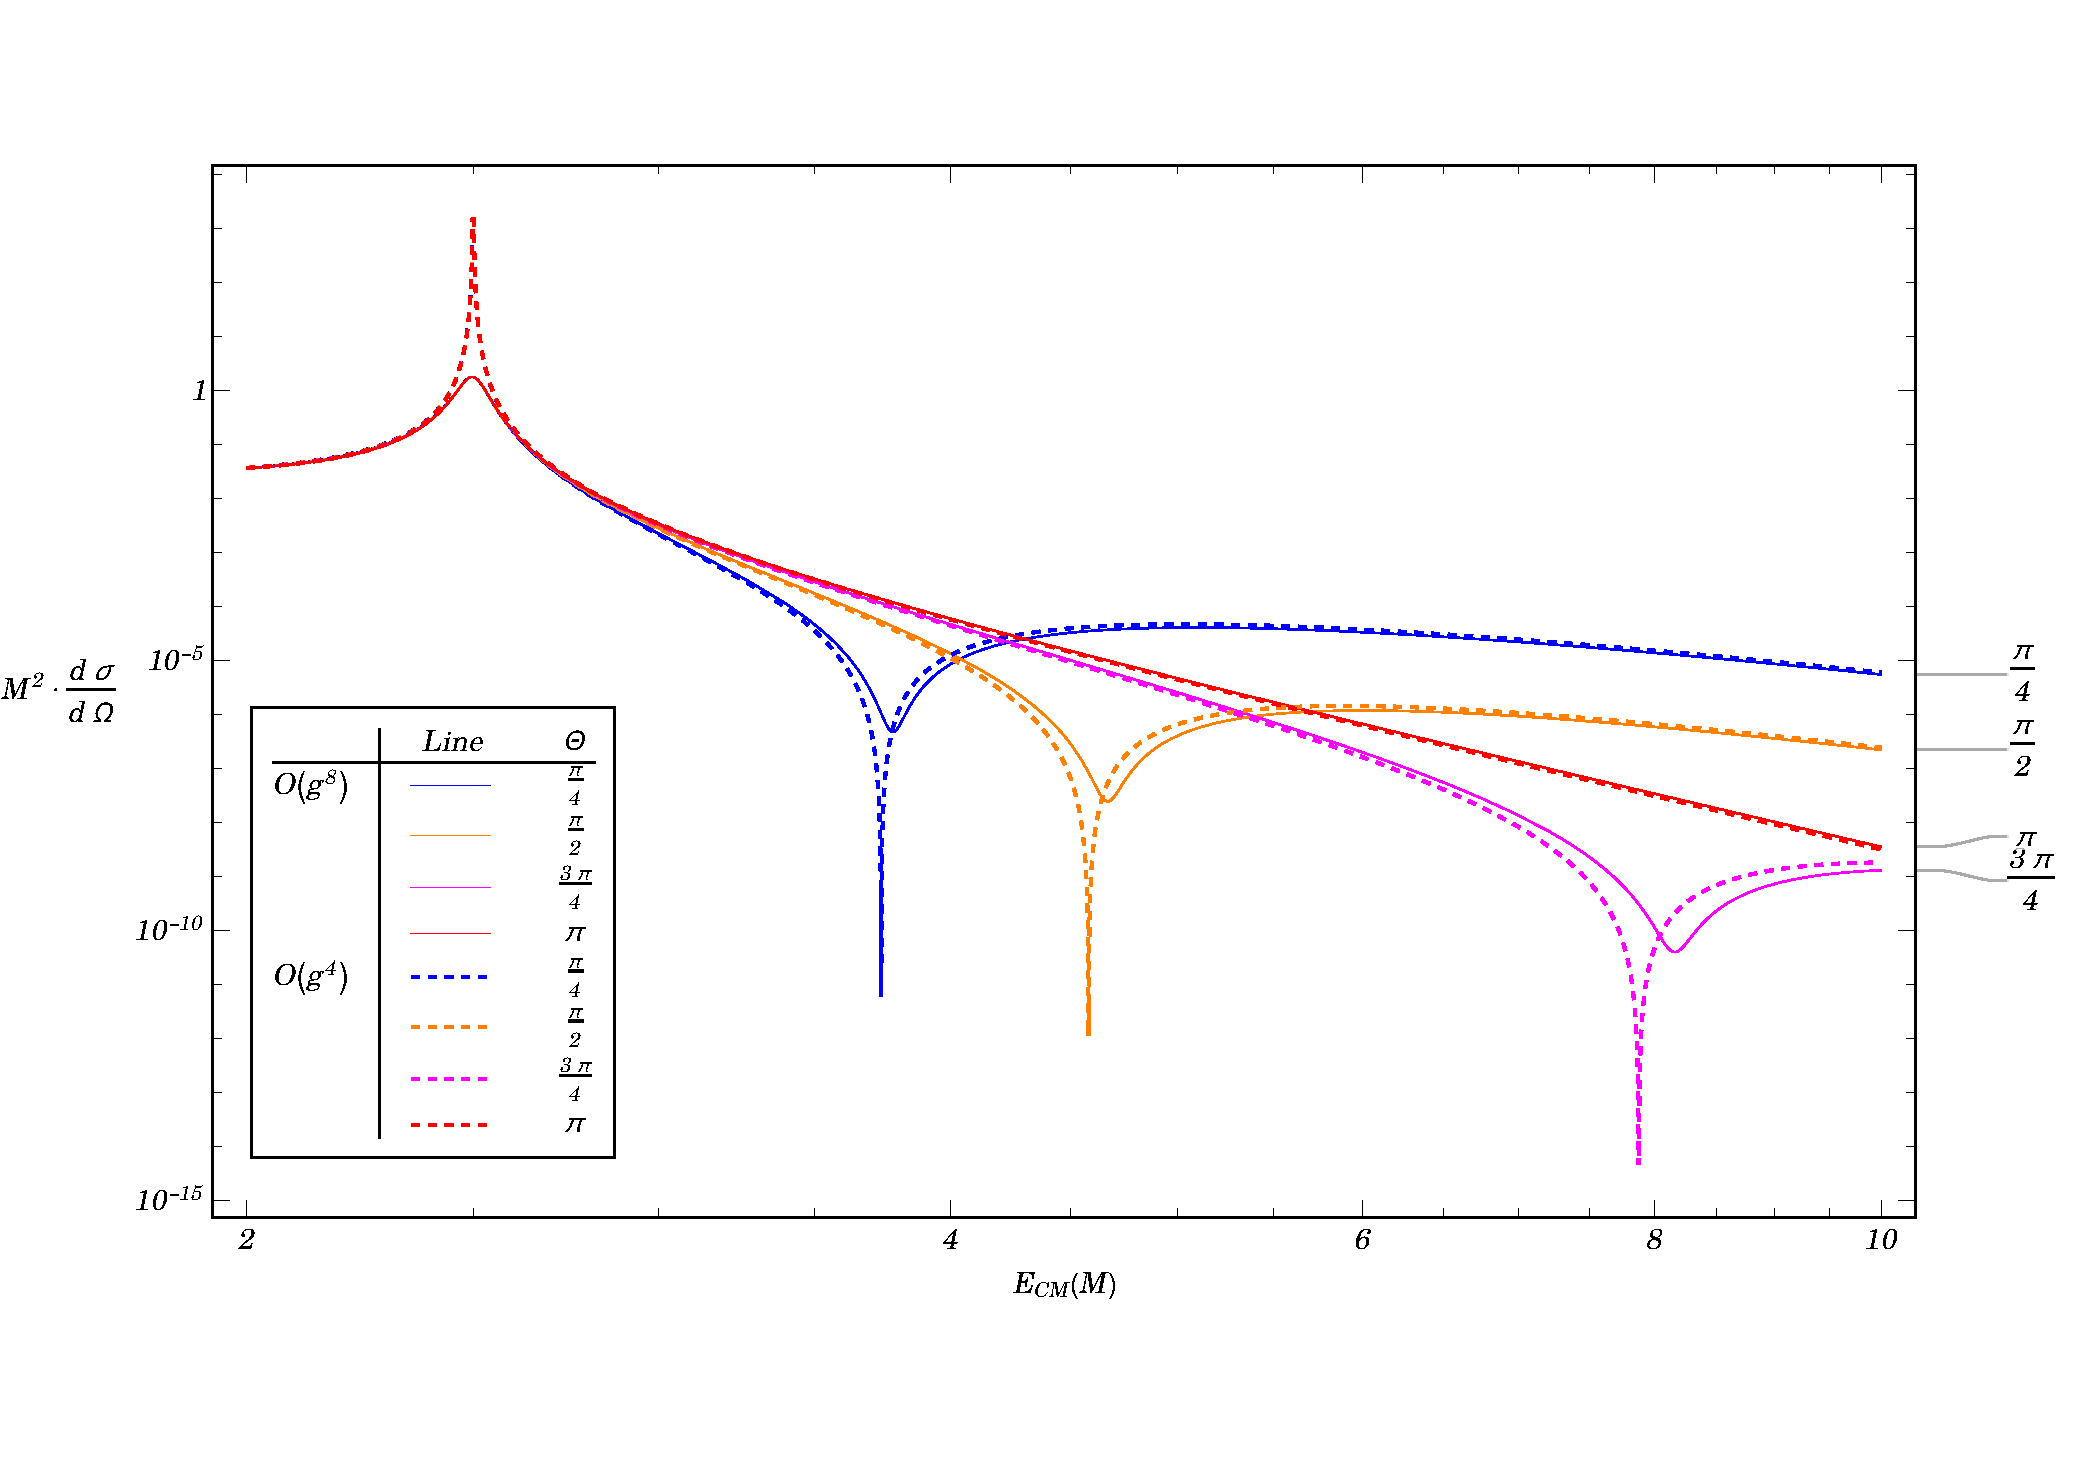
\includegraphics[width=15cm, height=11cm]{UnStableMeson-Illustration}
\caption{Scattering cross section versus total scattering energy for the strongly coupled theory ($g = 4 M$) at both tree-level and the one-loop level in the unstable meson regime $m = 2.5 M$. Curves show the scattering amplitude at a fixed scattering angle. Solid lines are the full one-loop calculation such that the cross section is exact to $O(g^8)$. Dashed lines are the tree-level result which is order $g^4$ in the scattering amplitude. The scale is log-log. Energies are expressed in multiples of the $\psi$ particle rest mass.} 
\label{Ill}
\end{center}
\end{figure}

\begin{figure}
\begin{center}
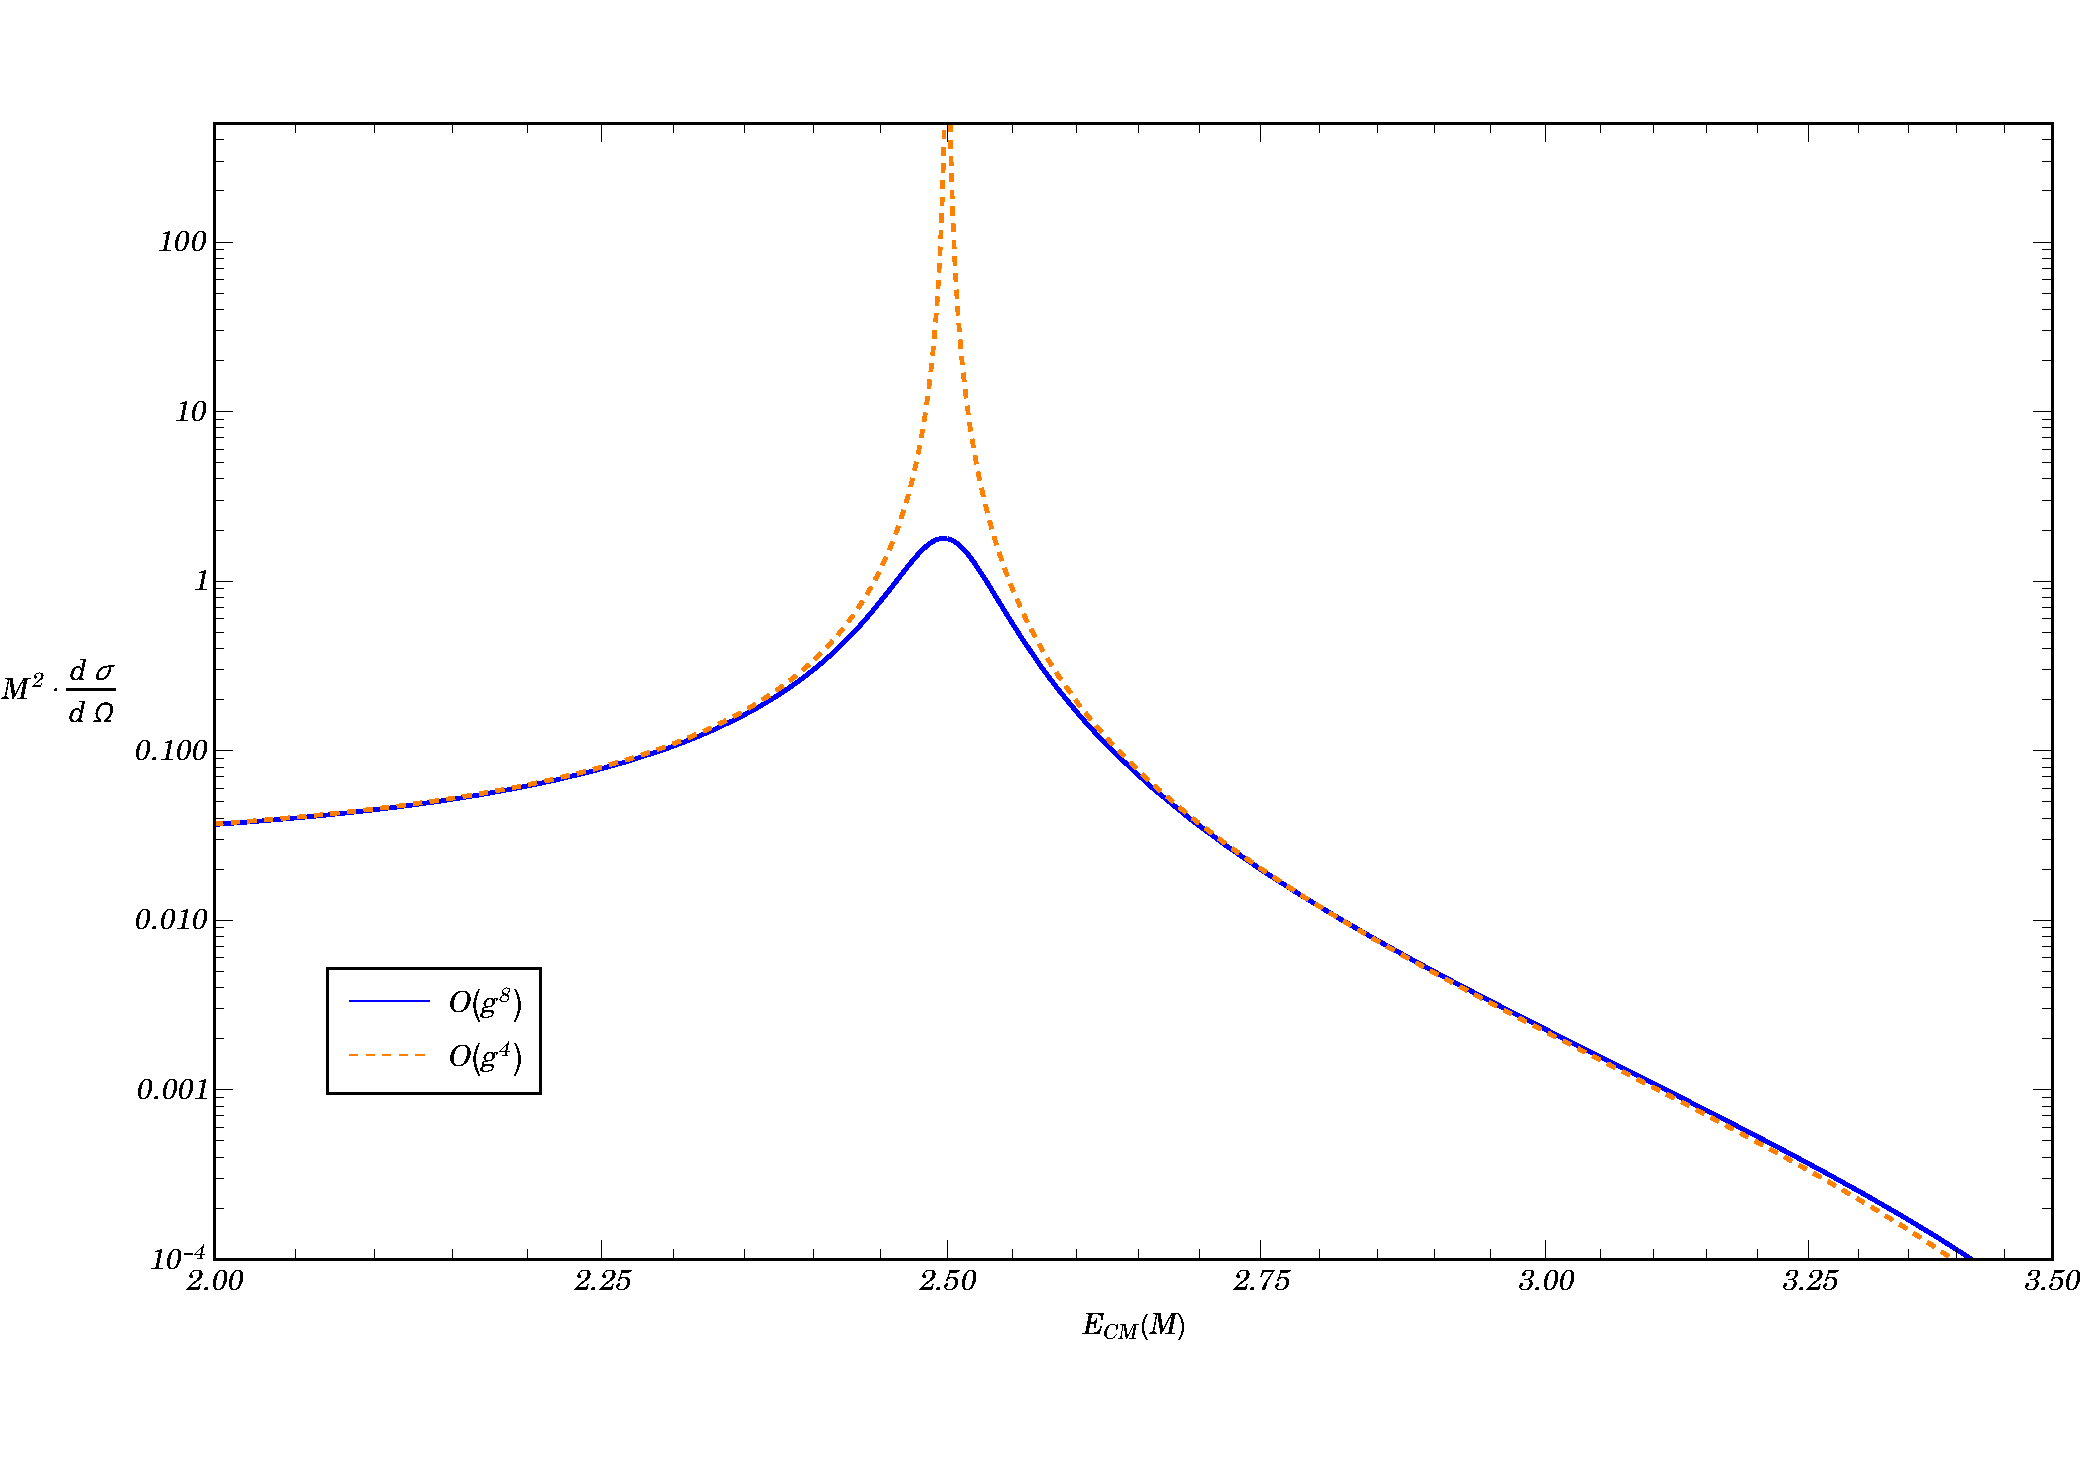
\includegraphics[width=15cm, height=11cm]{Resonance-Illustration}
\caption{Closeup of scattering cross section resonance due to (nearly) on-shell virtual meson in the strongly interacting ($g = 4 M$) unstable meson regime with $m = 2.5 M$. The scattering angle is fixed at $\Theta = \frac{\pi}{4}$. Scattering cross sections are plotted on a log scale. Total scattering energy is expressed in multiples of the $\psi$ rest mass.} 
\label{IllResonance}
\end{center}
\end{figure}

\end{document}
